\documentclass[11pt,en]{elegantpaper}
\title{Quantitative Risk Management Project 6}
\author{Qijun Yang \\ Duke University}
\institute{\href{https://fintech.meng.duke.edu}{Financial Technology at Duke University}}
\version{1.0}
\date{Mar. 17, 2023}

% cmd for this doc
\usepackage{array}
\usepackage{listings}
\usepackage{graphicx}
\usepackage{subfigure}
\newcommand{\ccr}[1]{\makecell{{\color{#1}\rule{1cm}{1cm}}}}

\addbibresource[location=local]{reference.bib} % reference file
\begin{document}
\maketitle

\section*{\textcolor{orange}{Problem 1}}

Assume you a call and a put option with the following
\begin{enumerate}
    \item Current Stock Price \$165
    \item Current Date 03/03/2023
    \item Options Expiration Date 03/17/2023
    \item Risk Free Rate of 4.25\%
    \item Continuously Compounding Coupon of 0.53\%
\end{enumerate}

Calculate the time to maturity using calendar days (not trading days).

For a range of implied volatilities between 10\% and 80\%, plot the value of the call and the put.

Discuss these graphs. How does the supply and demand affect the implied volatility?

\section*{\textcolor{orange}{Answer}}
Given the underlying price, the current date, the expiration date, the risk-free rate, and the cost of carry, we could obtain the price of the European call or put option if we had the volatility and the strike price.

Varying the volatilities from 10\% and 80\% and using the Generalized Black\-Scholes Model to get the price, we plot the two numbers by setting different strike prices for the call and put options.


\begin{figure}[htbp]
    \centering
    \subfigure[Figure A]{
    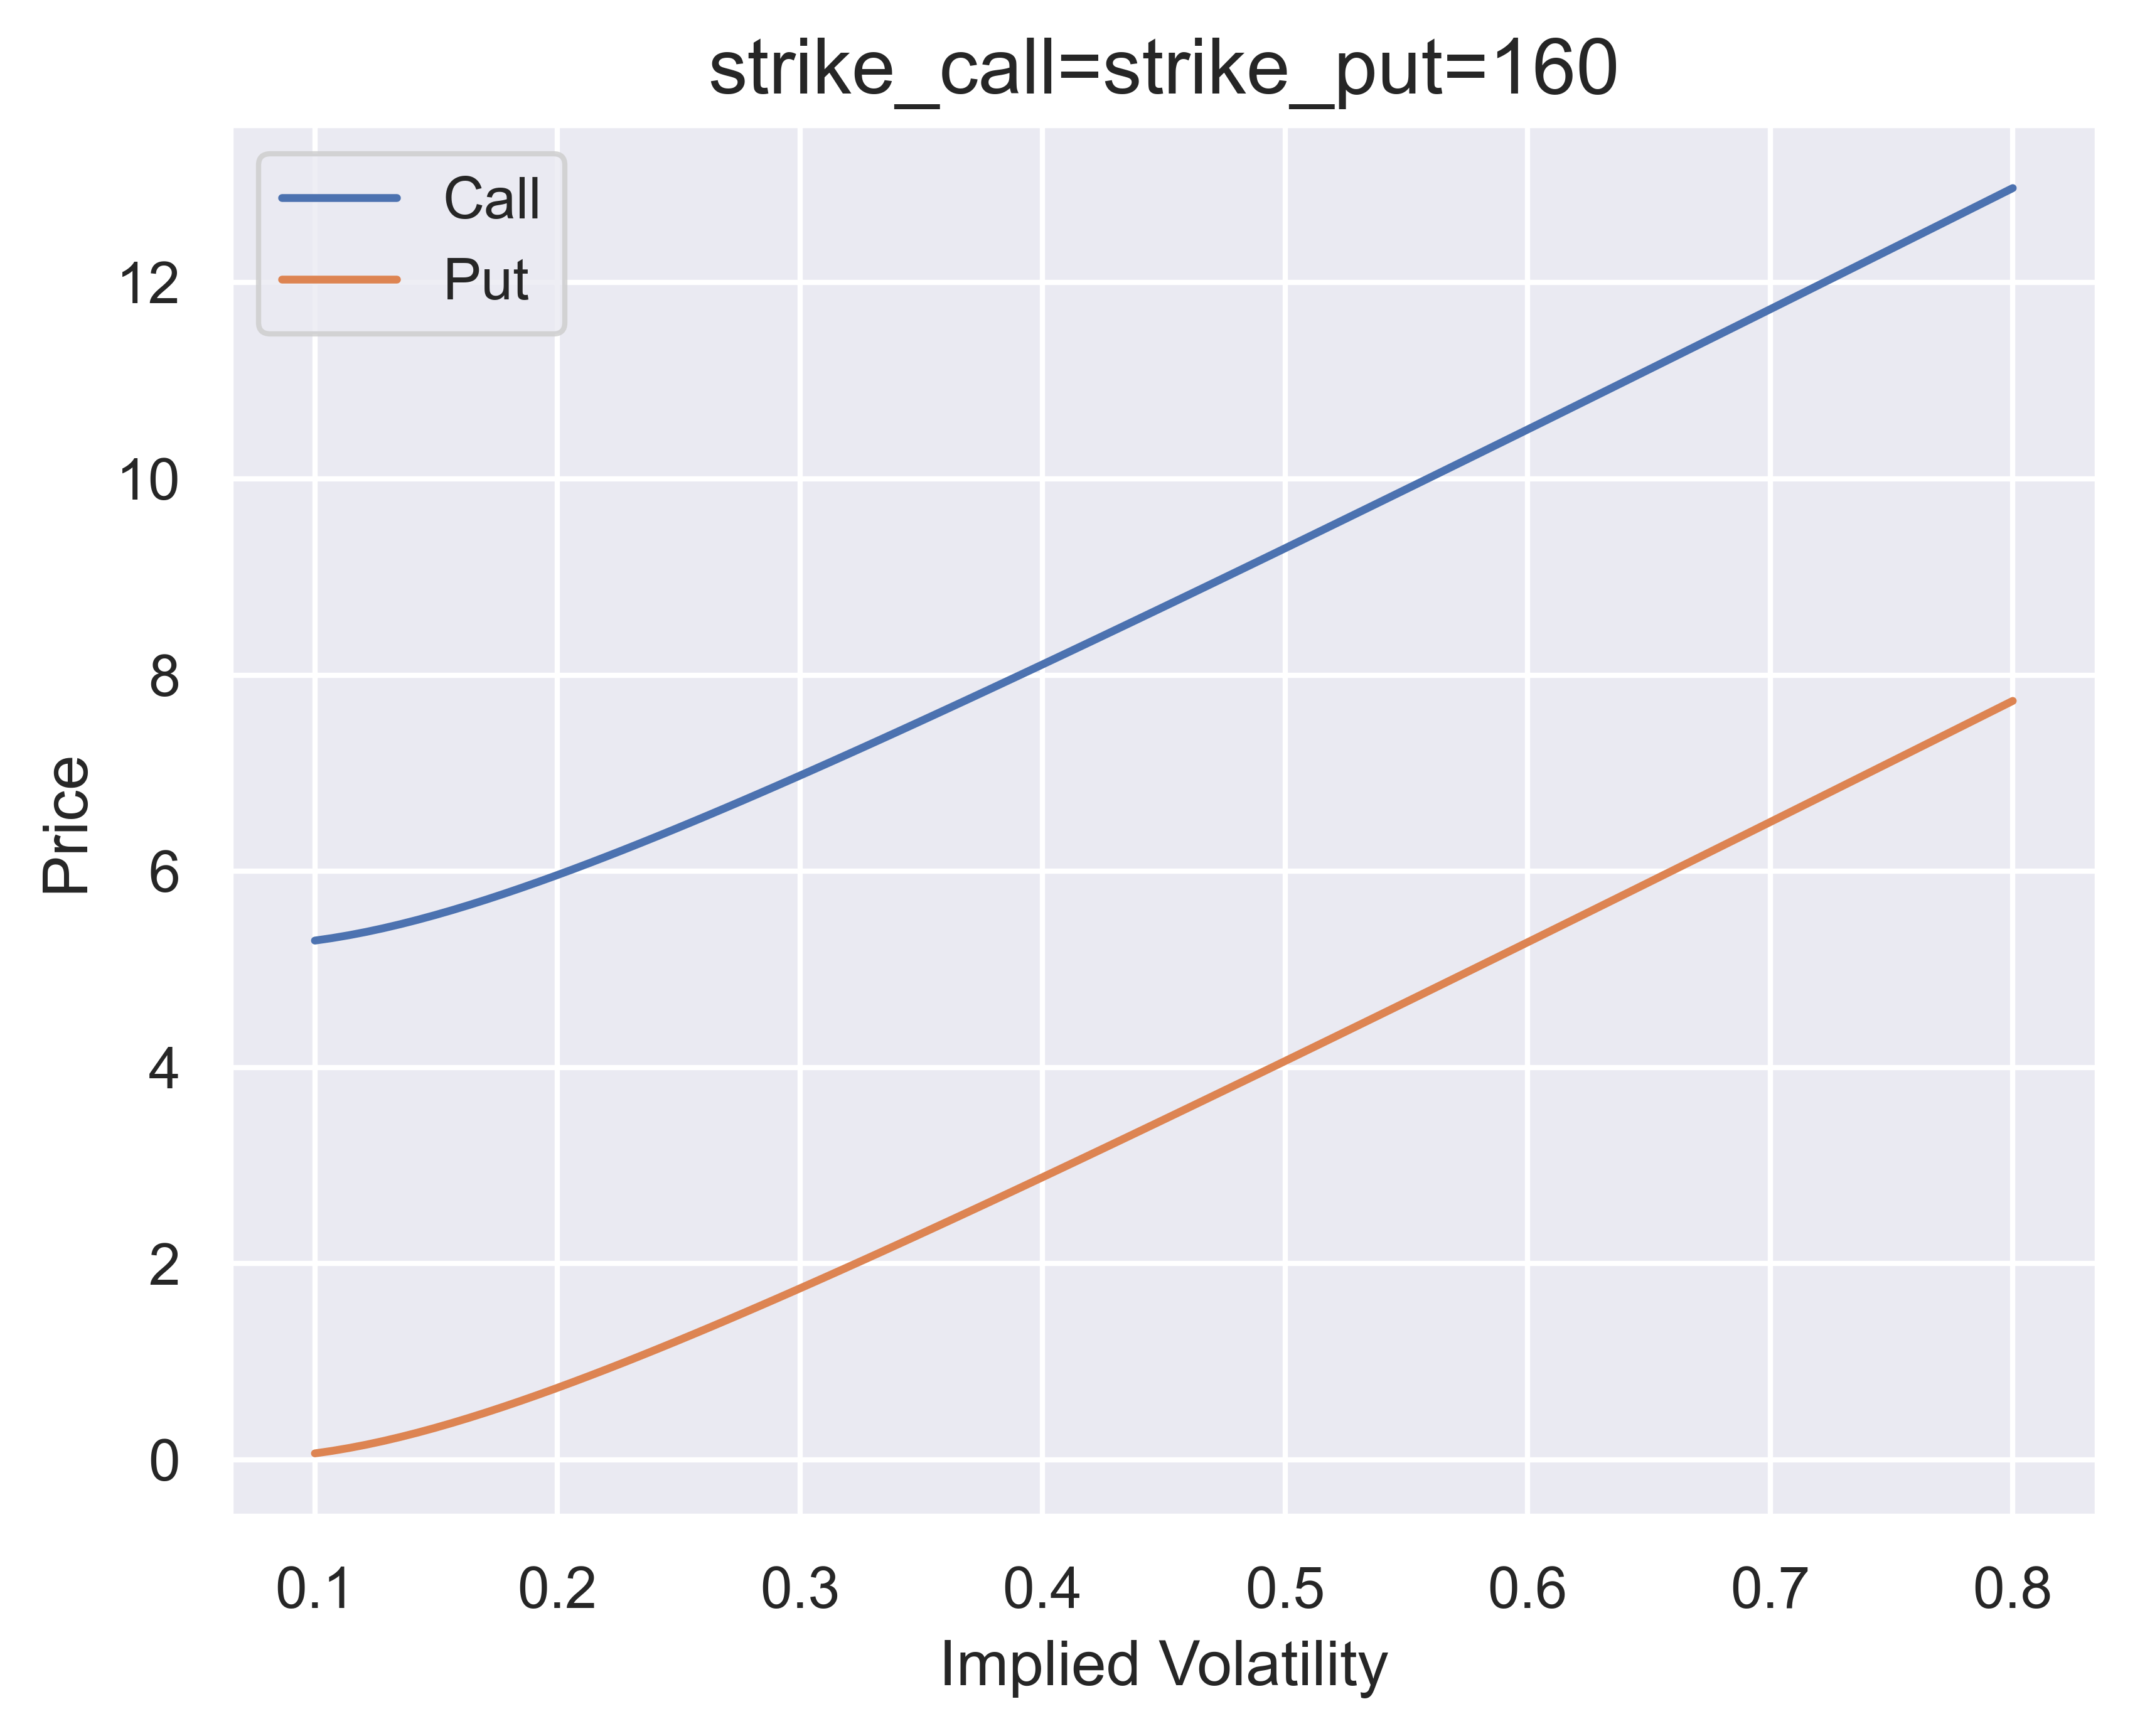
\includegraphics[width=0.45\textwidth]{./image/image_1/strike_call=strike_put=160.png} 
    }
    \quad
    \subfigure[Figure B]{
    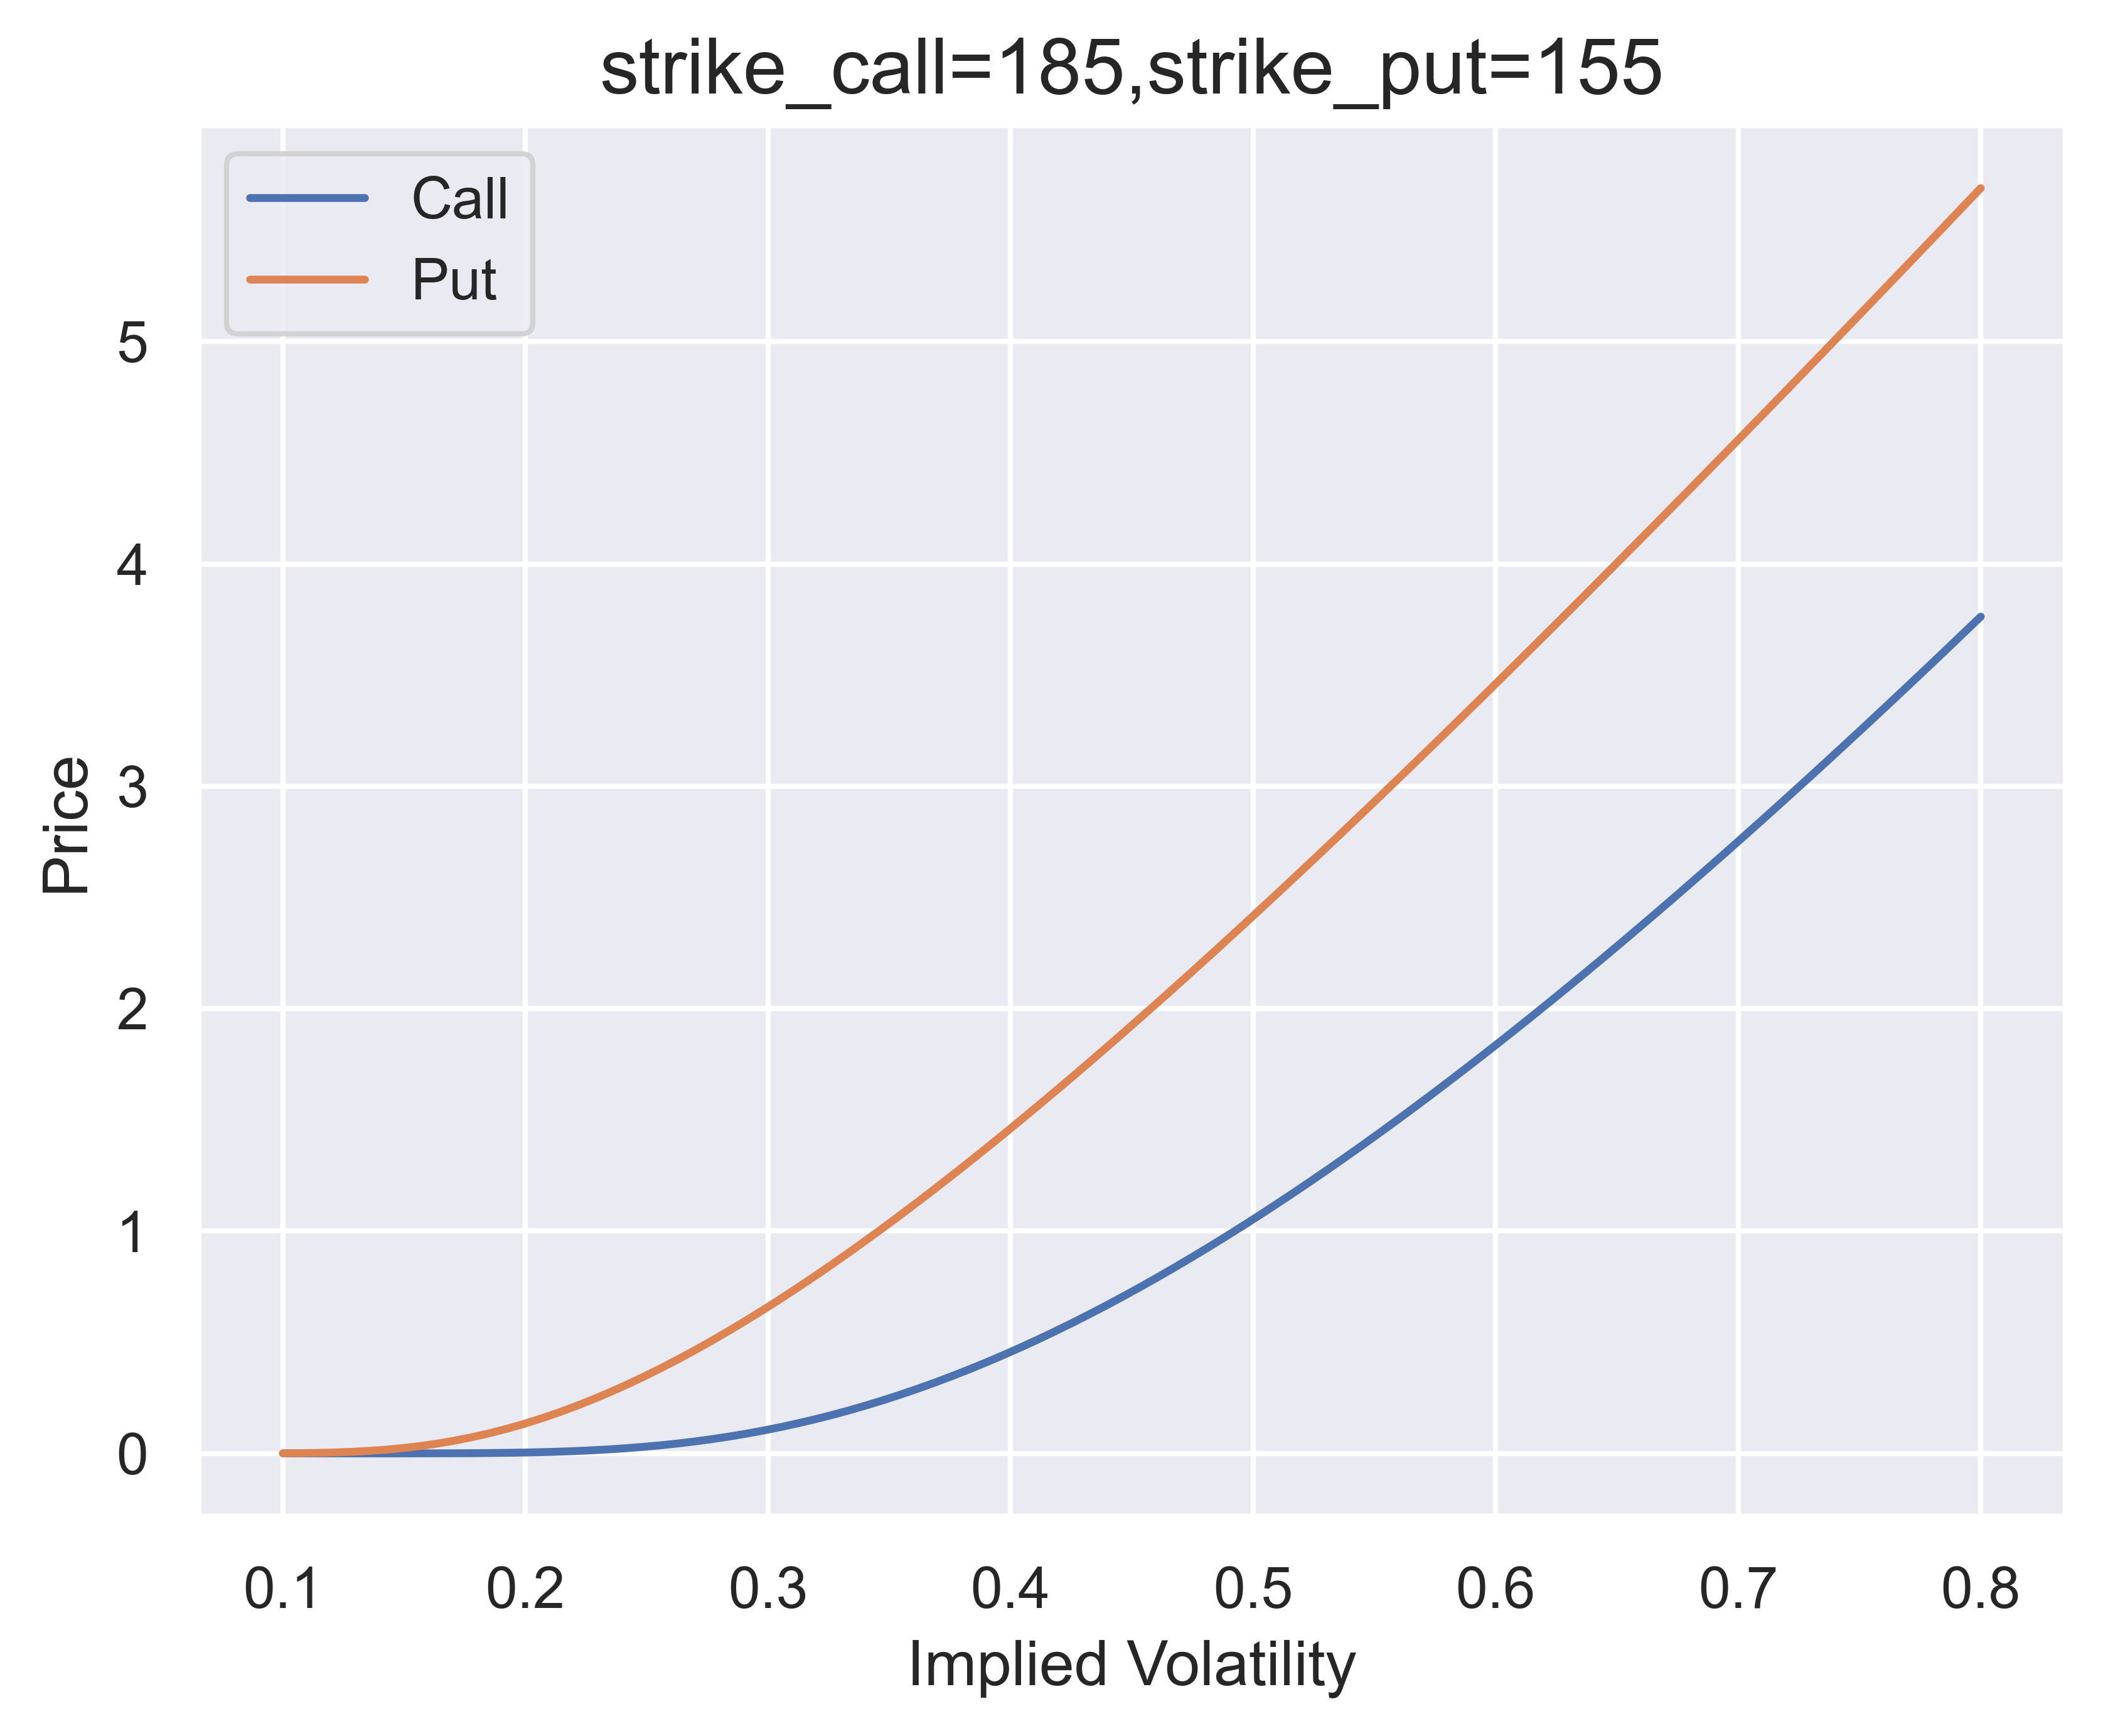
\includegraphics[width=0.45\textwidth]{./image/image_1/strike_call=185,strike_put=155.png} 
    }
    \caption{Option Price due to different implied volatilities}
\end{figure}

\subsection*{\textcolor{orange}{Finding:}}
From the figures, we can see that the price of the option will increase as its implied volatility increases, regardless of the strike price. 

The higher the volatility of the underlying asset, the more chances it has to enter the profit zone, resulting in a higher value. 

To elaborate, the value of an option can be divided into two parts: intrinsic value and time value. 

The intrinsic value of an option is the difference between the current price of the underlying asset and the strike price of the option. 

The time value of an option represents the potential for the underlying asset price to move in a favorable direction before the option expires. When volatility increases, the potential for the underlying asset price to move in a favorable direction also increases, which can lead to a greater time value for the option.

\textbf{As for supply and demand of option}, they work together to determine the price of option and price. If there is more demand for the option than supply in the market, the price of the option goes up, which in turn indicates that the implied volatility is increasing.

Let's take a look at the call option to make our analysis reasonable.

\textbf{The reason this will happen is that} if people think that the underlying asset of the call option will go up to some extent that will satisfy their expectations for returns, they will go to buy the option. That certain amount represents the market's expectations about the future price movements of the underlying asset, which is reflected in the implied volatility of the option. If investors expect the price of the underlying asset to be more volatile in the future, the implied volatility of the option will increase and the option price will rise.

Implied volatility is a measure of the market's expectation for the future volatility of the underlying asset, as implied by the prices of options on that asset.

\textbf{The relationship between supply and demand for the option determines the market's expectations of implied volatility, which can be reflected in the option price.}


\section*{\textcolor{orange}{Problem 2}}
Use the options found in AAPL\_Options.csv
\begin{enumerate}
    \item Current AAPL price is 151.03
    \item Current Date, Risk Free Rate and Dividend Rate are the same as problem \#1.
\end{enumerate}

Calculate the implied volatility for each option.

Plot the implied volatility vs the strike price for Puts and Calls. Discuss the shape of these graphs. What market dynamics could make these graphs?

There are bonus points available on this question based on your discussion

Take some time to research if needed.
    
\section*{\textcolor{orange}{Answer}}
Given the price of the underlying, the current date, the expiration date, the risk-free rate, the cost of carry, the different strike prices, and the corresponding option price, we could obtain the implied volatility of the underlying by applying an optimization algorithm to the generalized Black-Scholes model.

Calculating all the implied volatilities and plotting those of the call and put options separately against the strike price, we get the following graph.

\begin{figure}[htbp] 
    \centering 
    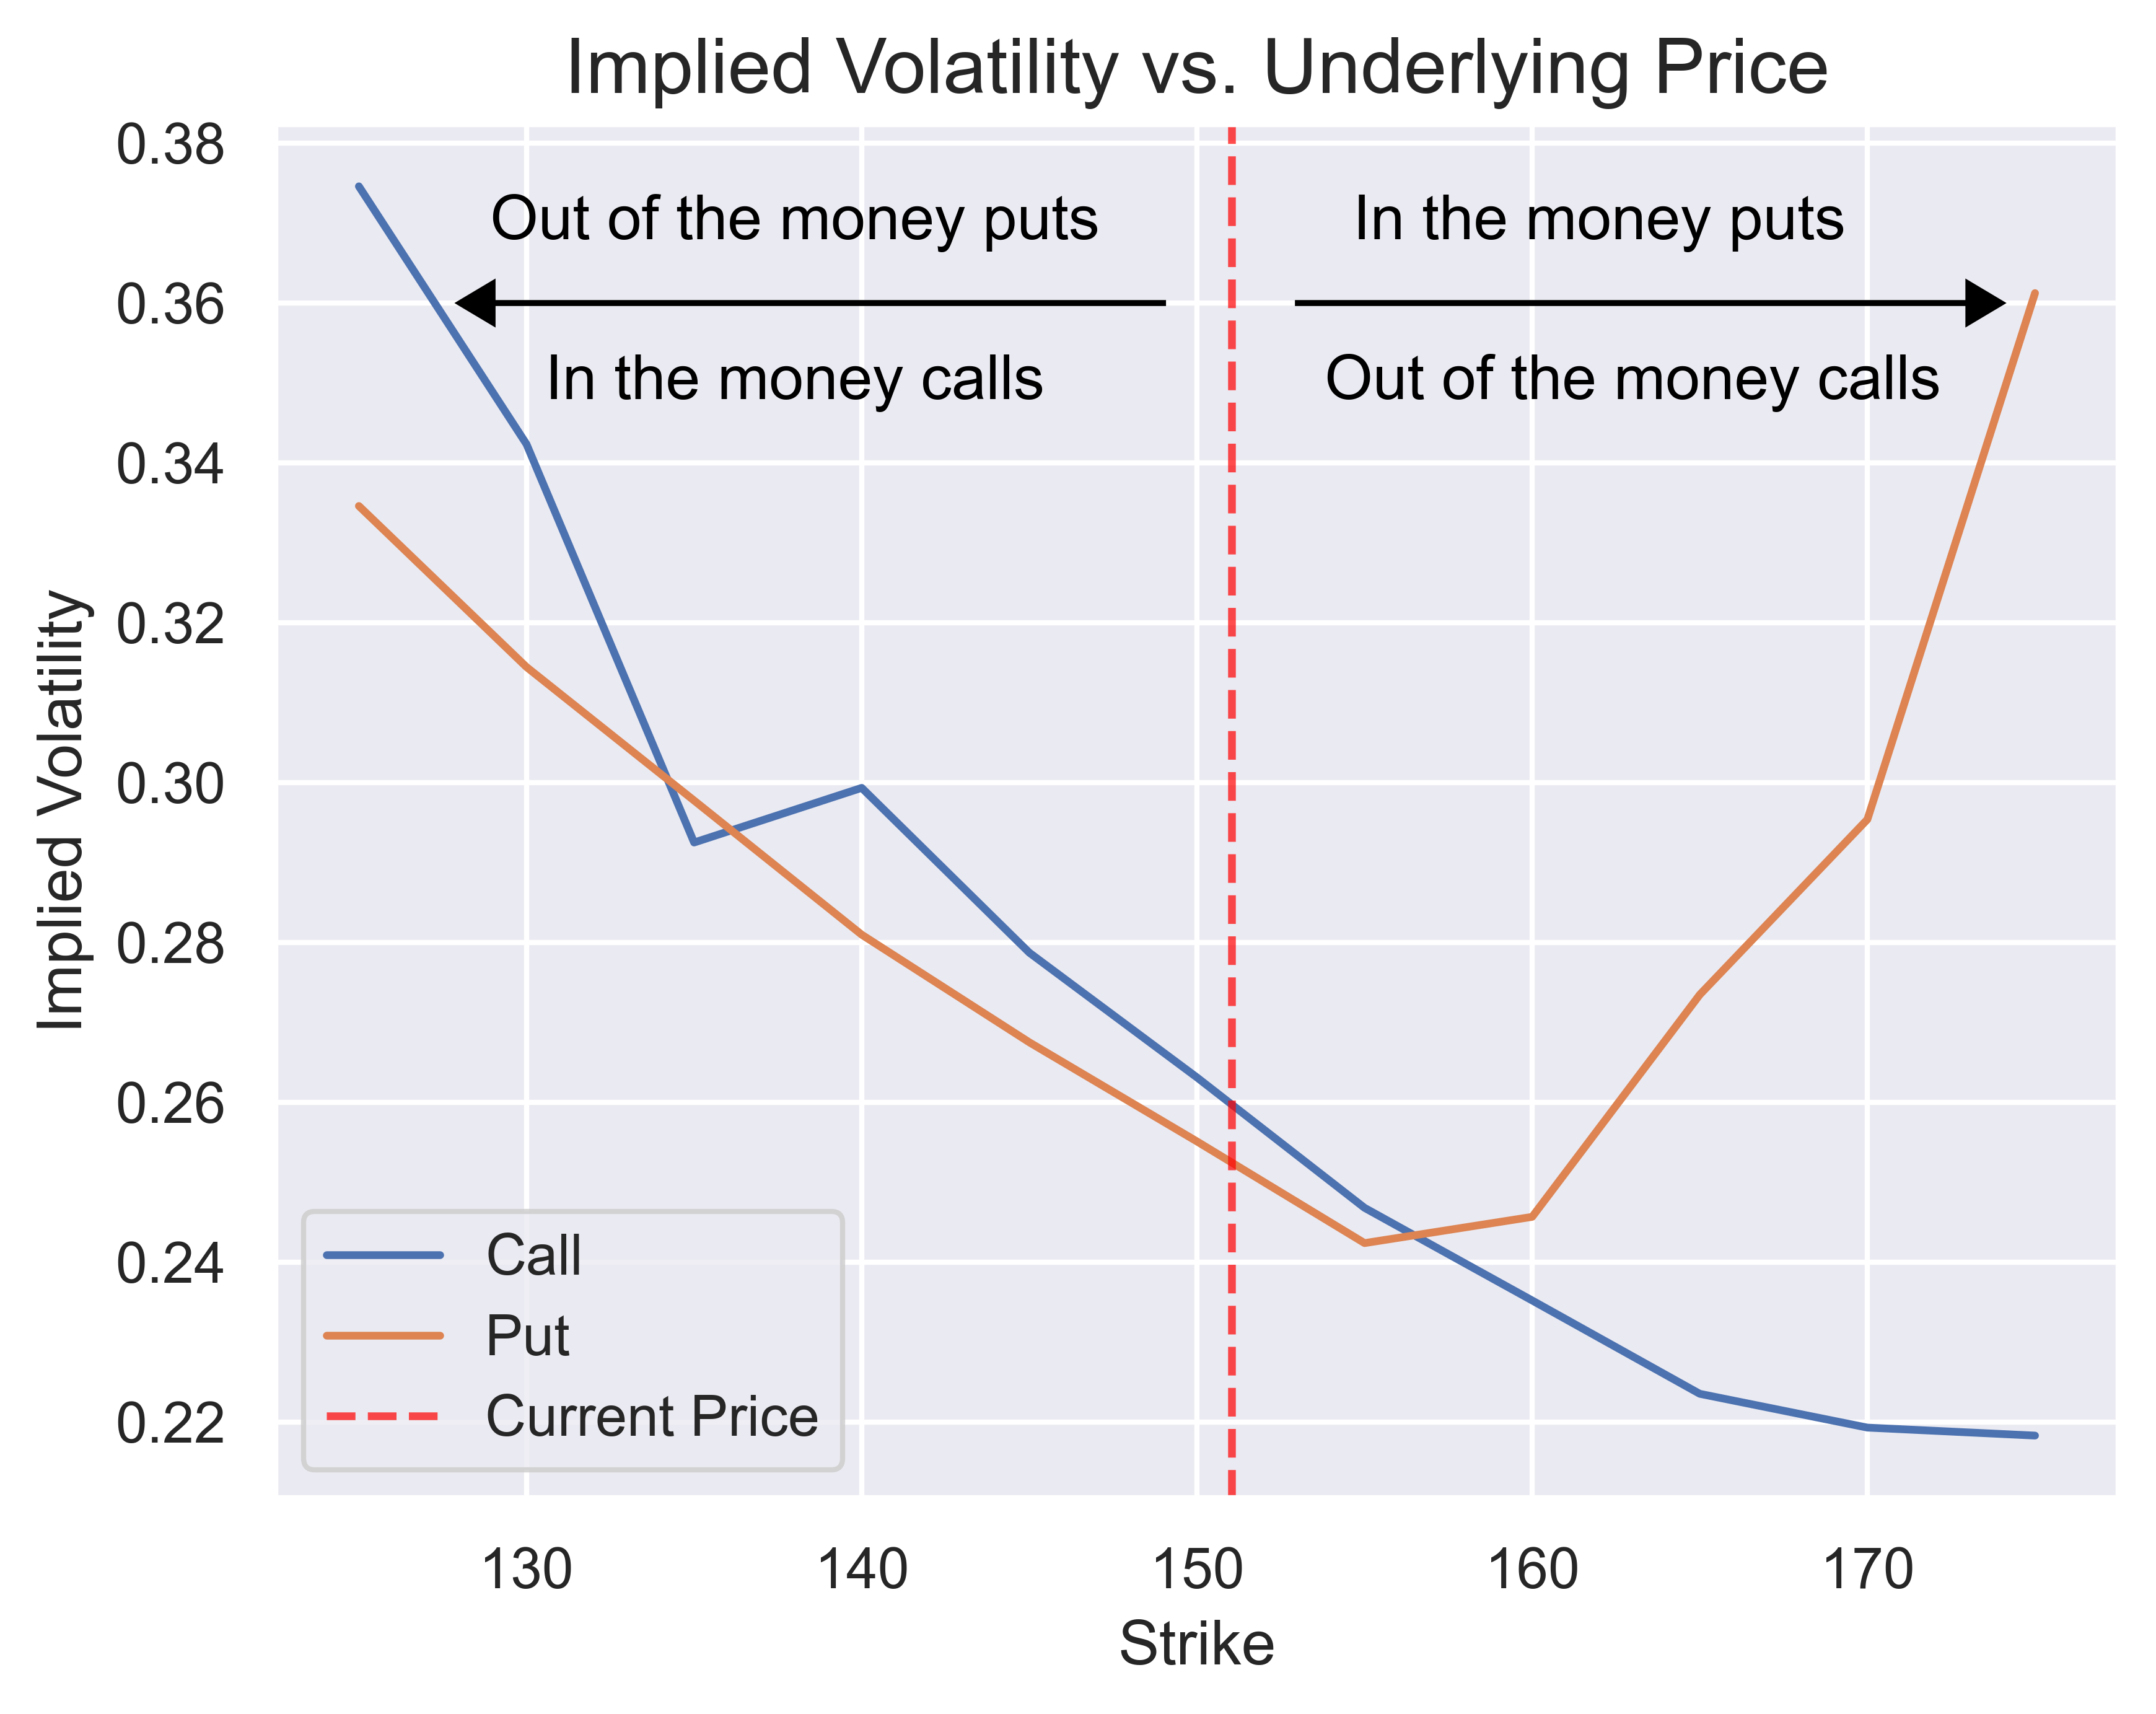
\includegraphics[width=0.6\textwidth]{./image/image_2/ImpliedVolatility.png} 
    \caption{Volatility Smile}
\end{figure}

\subsection*{\textcolor{orange}{Discussion}}

We can see that the volatility curve of call and put is not flat. The volatility of the put is like a smile. The graph shows higher implied volatility for put options with strike prices significantly above or below the current market price of the underlying asset. Such a phenomenon is \textbf{volatility smile}. The curve is also \textbf{non-symmetrical} and we could easily see that the call and put curves are \textbf{negatively skewed}.

To find out why this happens, we need to review the \textcolor{orange}{\textbf{assumptions of the Black-Scholes model}}:
\begin{enumerate}
    \item \textbf{Efficient Markets}: The model assumes that financial markets are efficient, meaning that all available information is already reflected in the price of the underlying asset.---- No arbitrage opportunities, no transaction fees, borrowing and lending at risk-free rates, and the ability to buy and sell shares.
    \item \textbf{Lognormal Distribution of Underlying Asset Price (Normal Returns)}: The model assumes that the price of the underlying asset follows a lognormal distribution, which means that it has a bell-shaped curve when plotted on a logarithmic scale.
    \item \textbf{Constant Volatility}: The model assumes that the volatility of the underlying asset is constant and does not change over time.
    \item \textbf{No dividends}: The model assumes that the underlying does not pay dividends during the life of the option.
    \item \textbf{Risk Free Interest Rate}: The model assumes that there is a risk-free interest rate that is known and constant over the life of the option.
    \item \textbf{European-style options}: The model is designed to price European-style options that can only be exercised on the expiration date of the option.
\end{enumerate}

There are many theories as to why the volatility smile happens. I will only list some of the reasons I find in this project.

\textcolor{orange}{\textbf{The reason of Volatility Smile}}:
\begin{enumerate}
    \item \textbf{Non-normal returns}:  The Black-Scholes model assumes that stock prices follow a log-normal distribution, meaning that price movements are symmetrical about the mean. In reality, however, asset prices are subject to jumps or sudden changes that cause prices to deviate from the log-normal distribution. The real distribution of underlying asset returns has a fat tail, which means that the implied volatility of OTM options is higher than that of ATM options. This is because the probability of large price movements increases as you move away from the current price of the underlying asset.
    \item \textbf{Market participants' perceptions of risk}: If market participants perceive a higher level of risk or uncertainty in the market, they may demand higher prices for options that offer protection against potential losses. This can lead to an increase in the implied volatility of options, particularly for ITM and OTM options.
\end{enumerate}
To prove the above reason, I calculate the returns of AAPL and use implied and normal distribution graph to illustrate and elaborate.

\begin{figure}[htbp]
    \centering
    \subfigure[Figure A]{
    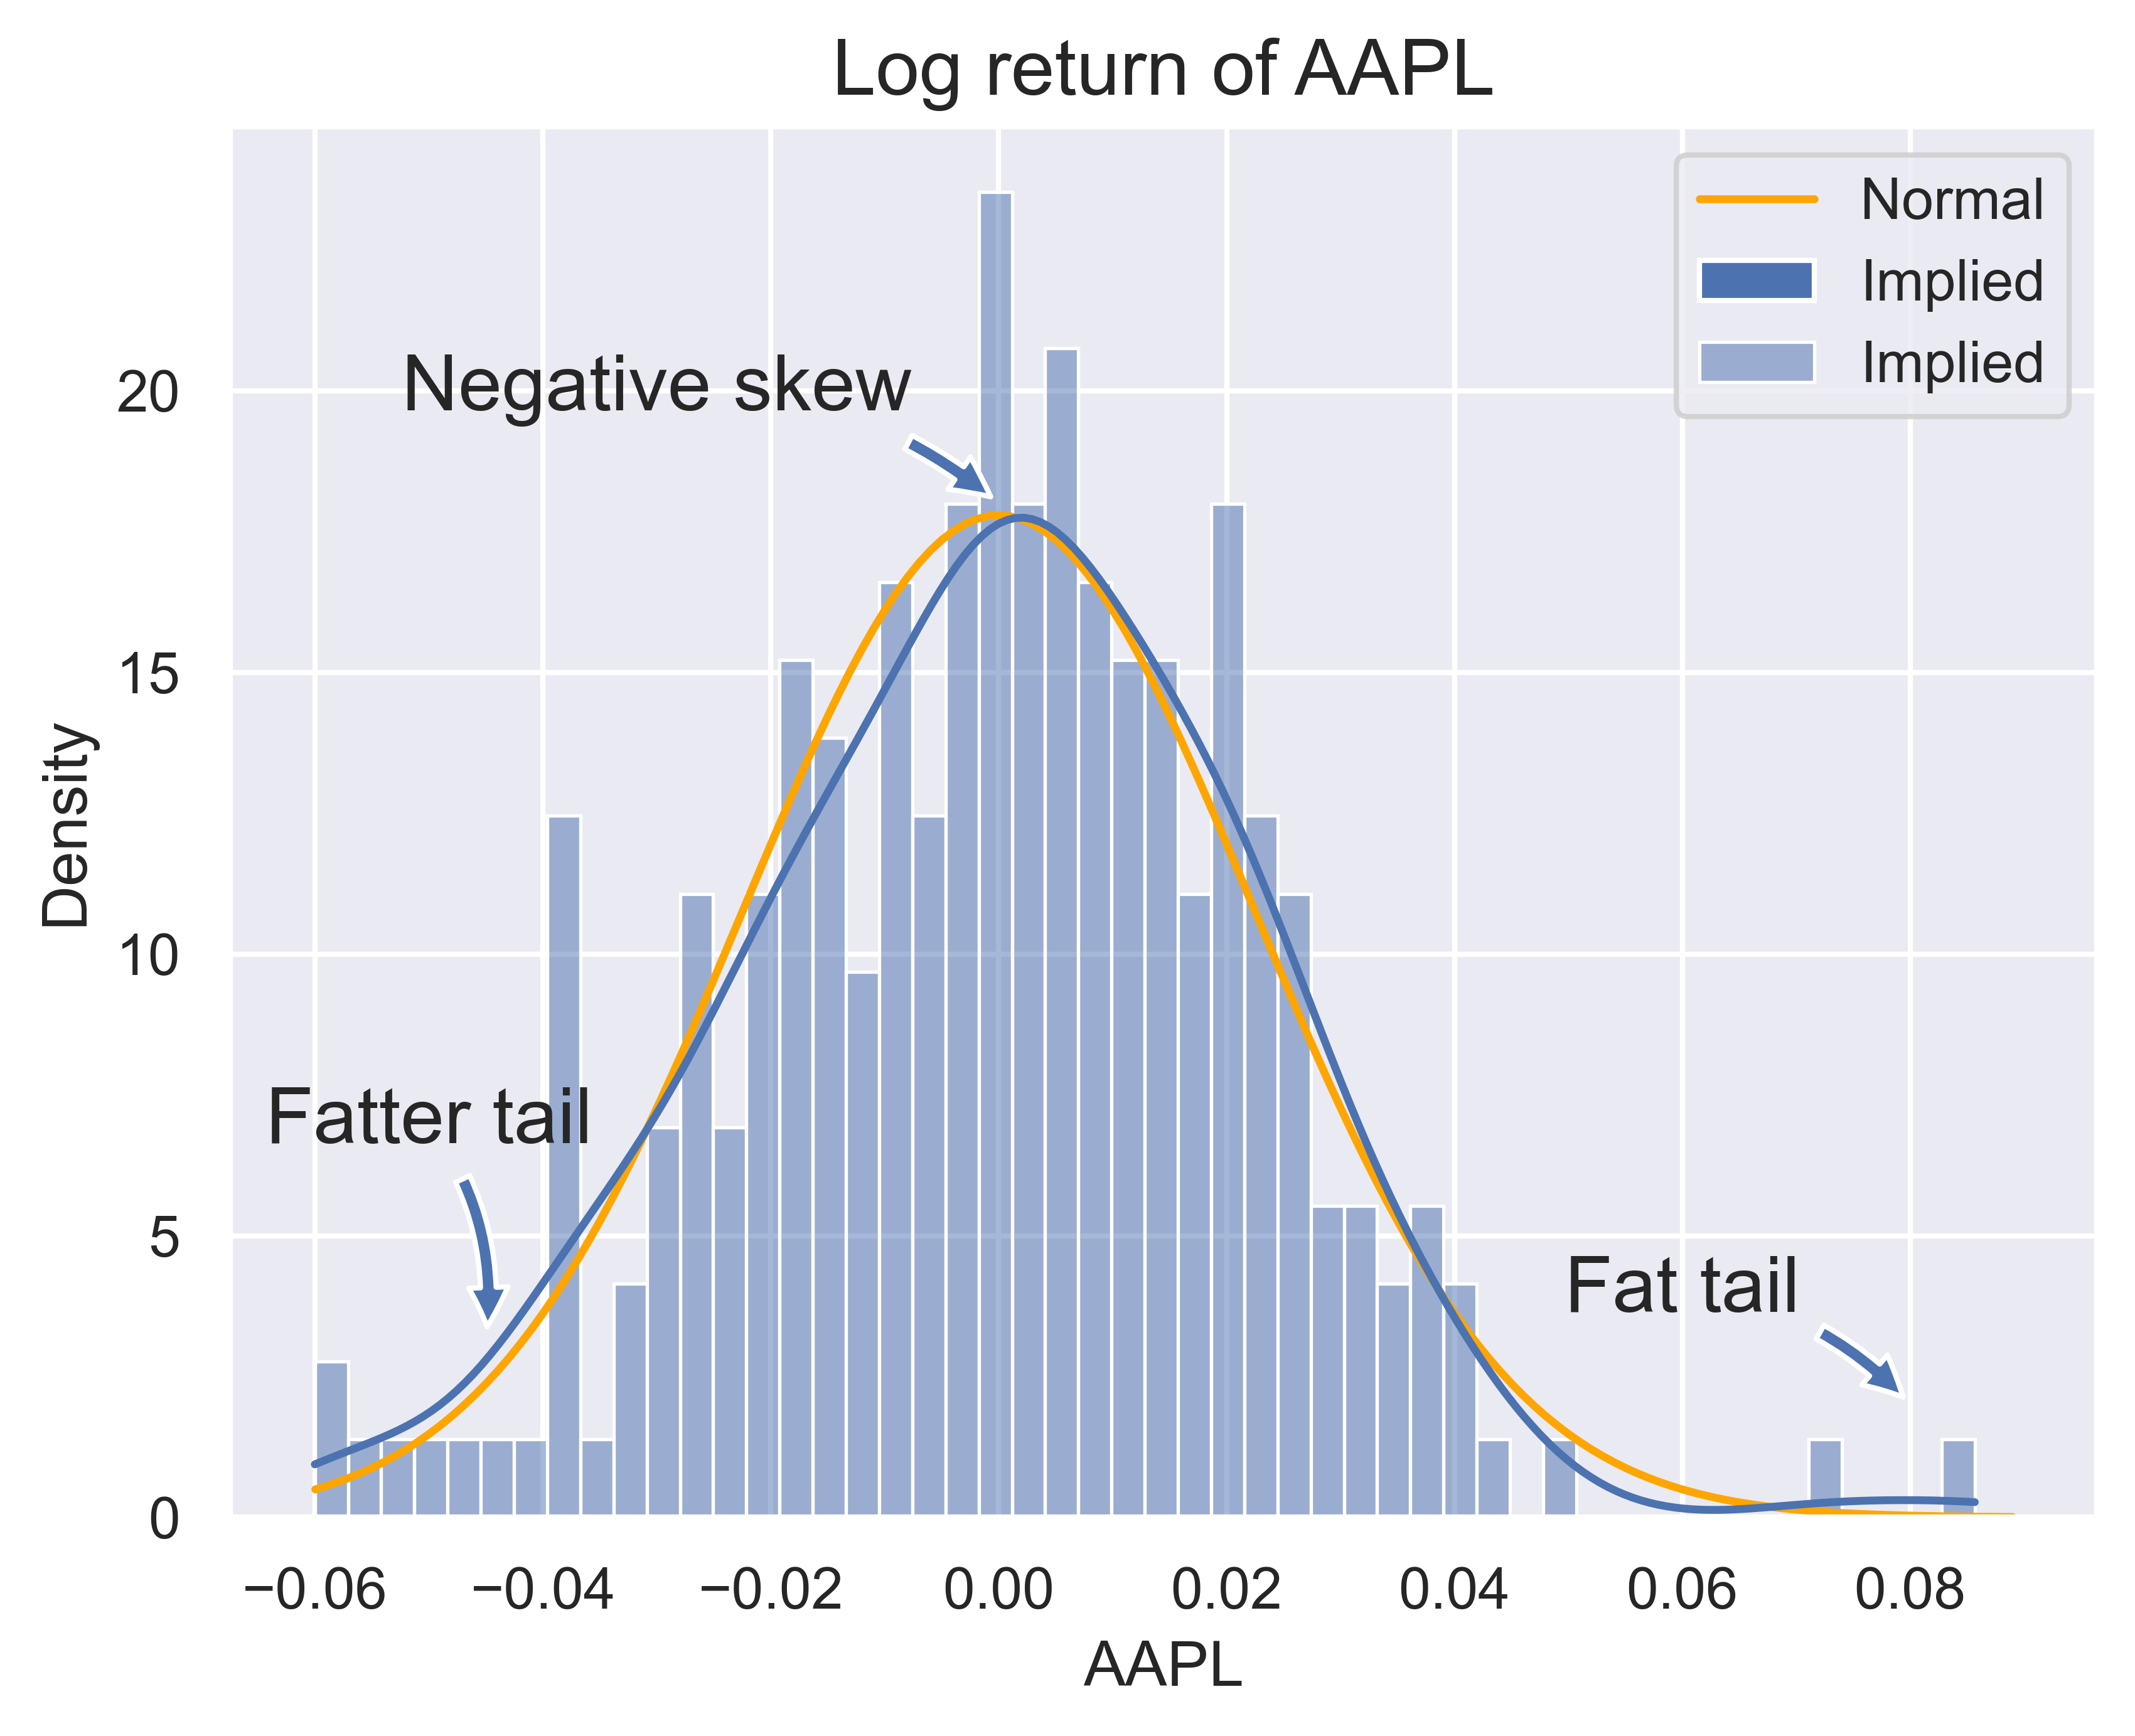
\includegraphics[width=0.45\textwidth]{./image/image_2/logReturn.png} 
    }
    \quad
    \subfigure[Figure B]{
    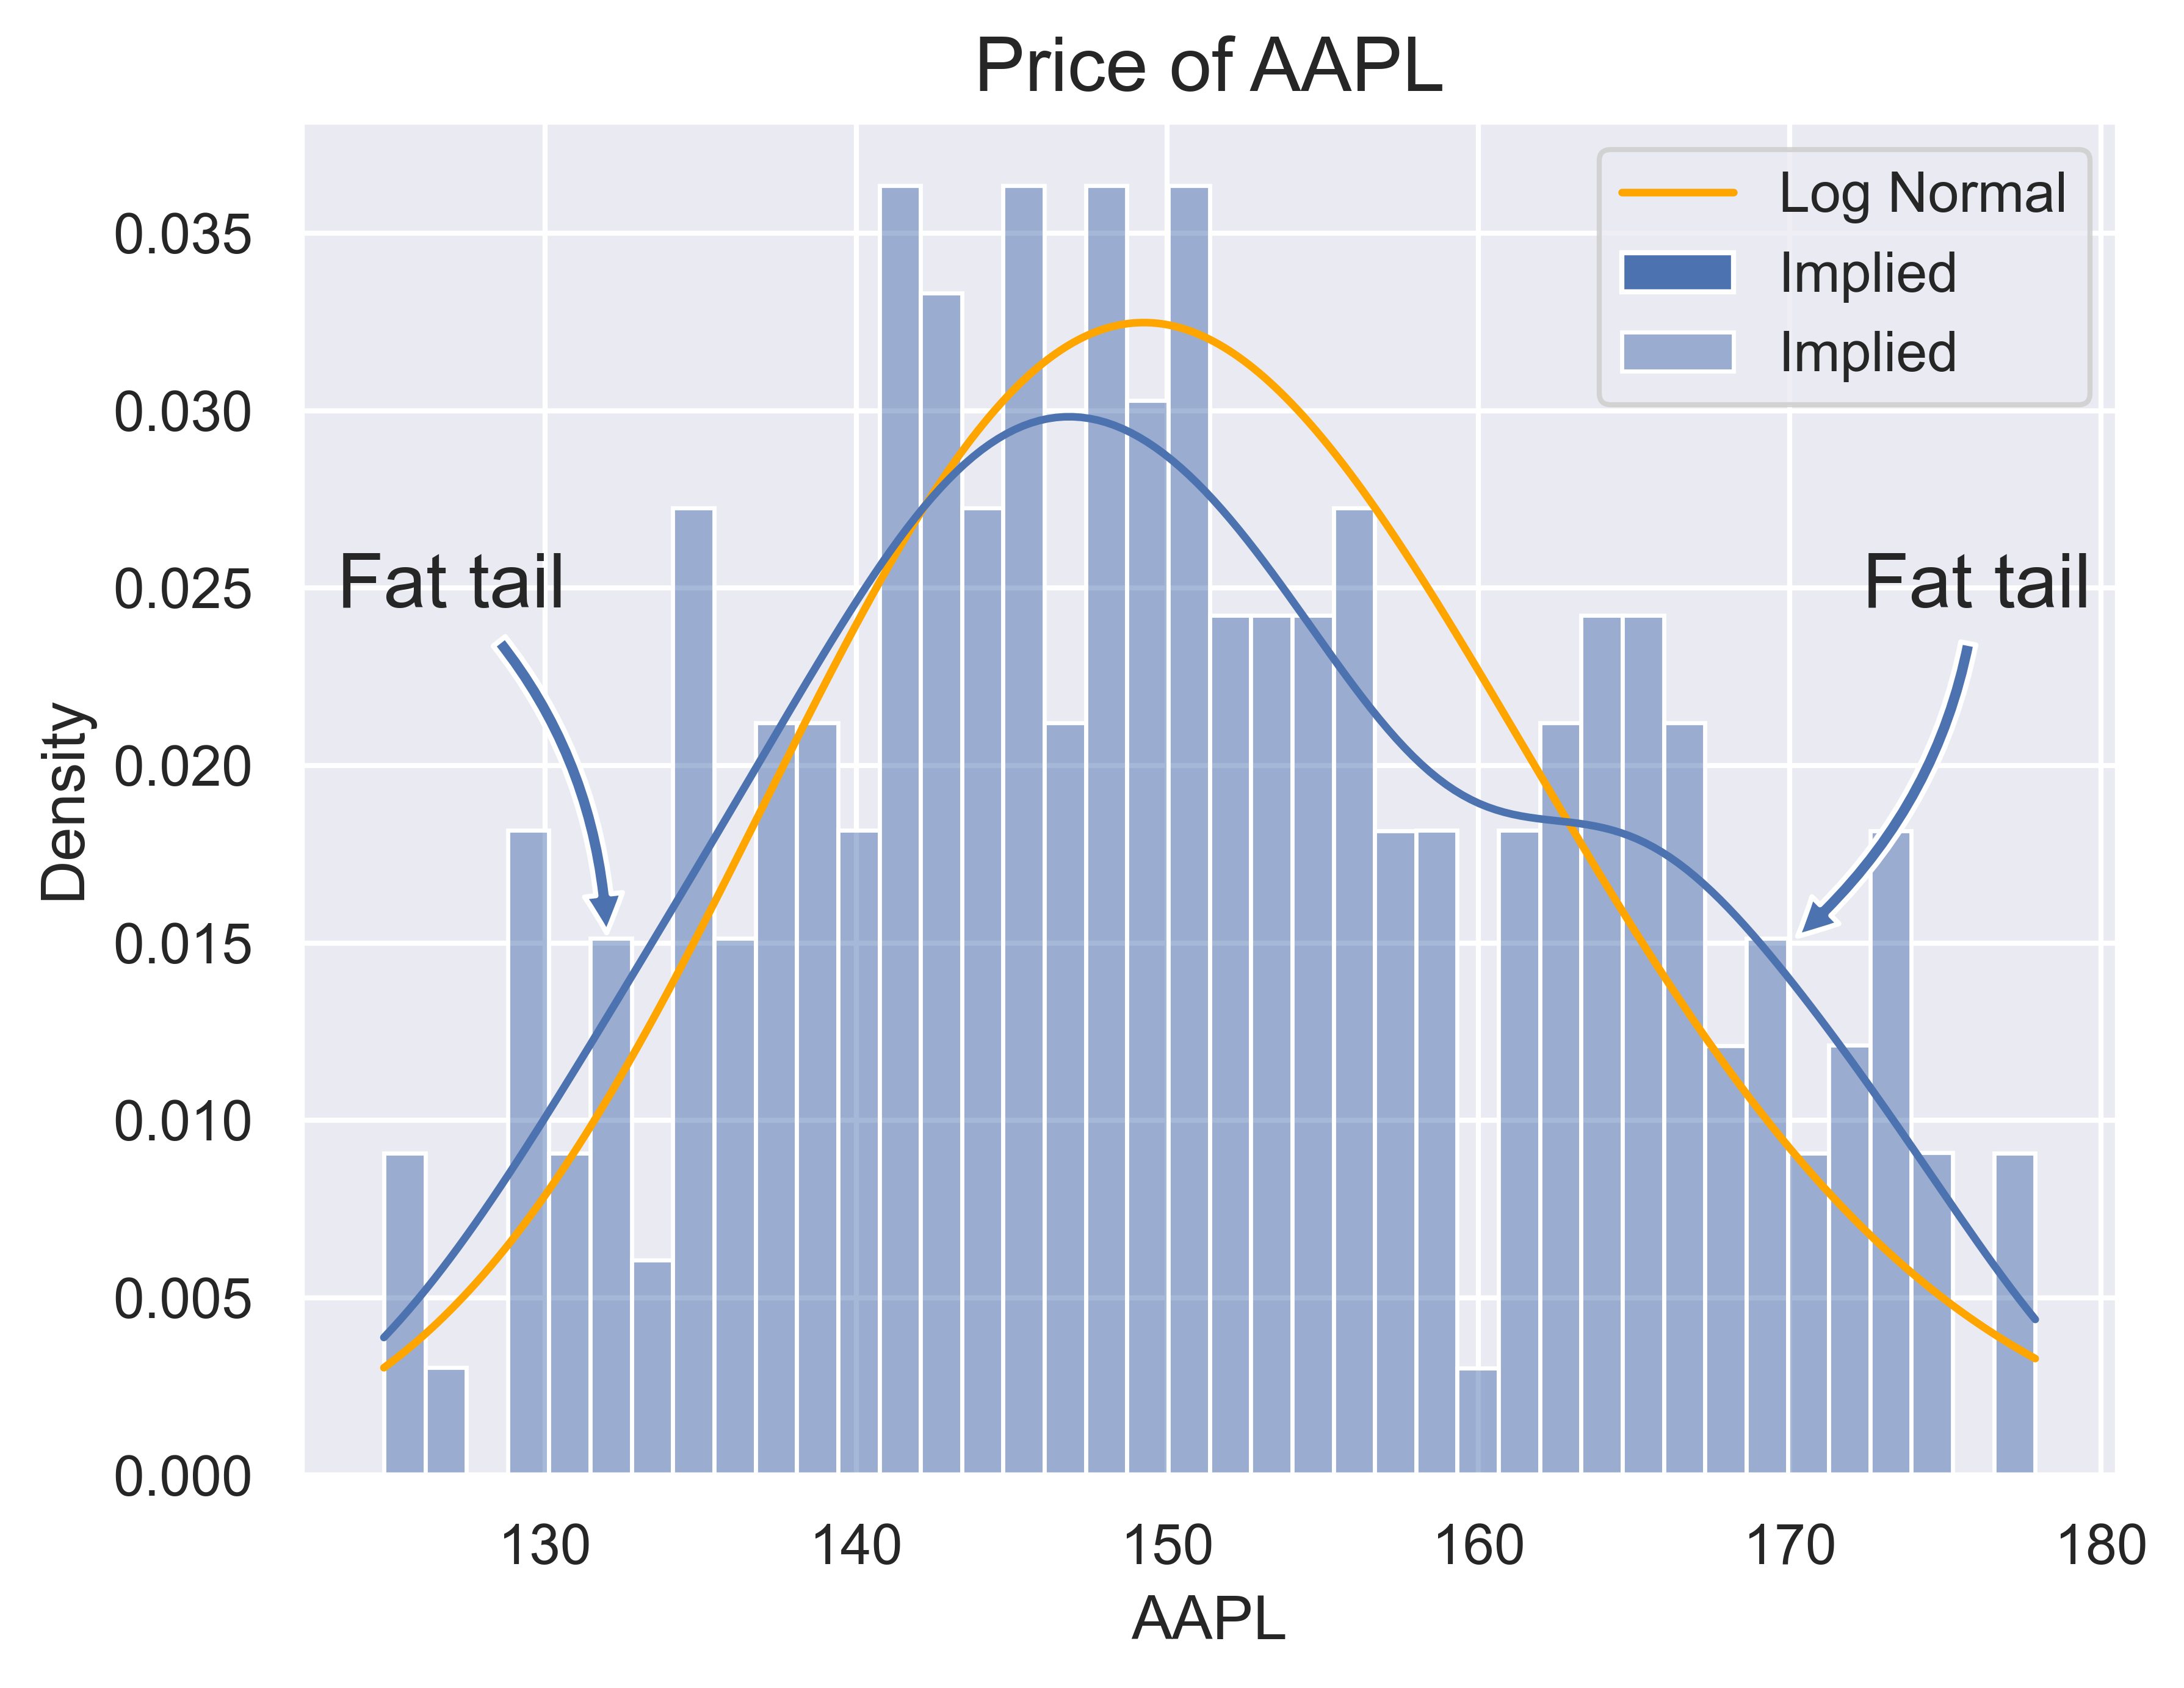
\includegraphics[width=0.45\textwidth]{./image/image_2/Price.png} 
    }
    \caption{Non-Normal Returns \& Non-Lognormal Price}
\end{figure}

From the graph, we can see that the real return distribution is different from the normal one. It's slightly negatively skewed and has a fatter tail on the left than on the right, although the right part also has a fat tail. Such a fat tail means a higher probability of extreme events that would have a large impact on the underlying price. Also from the price graph we could find that the price is not lognormally distributed and also has a fat tail.

\textcolor{orange}{\textbf{The negatively skewed reuturns result from several reasons. }}
\begin{enumerate}
    \item \textbf{Leverage effect}: When the price decreases, the denominator of the return decreases, which increases the rate of loss. Therefore, this effect is called the leverage effect, which increases risk. As stock prices fall, leverage increases, risk increases, and volatility increases. The resulting distribution of stock price volatility is relatively fat on the left and lean on the right.
    \item \textbf{Volatility feedback effects}: When volatility increases as in (1), investors take on more risk and expect higher returns.
\end{enumerate}

The negative skew and fat tail returns allow volatility to vary according to the different strike prices. 

\textcolor{orange}{\textbf{About the Equity Market}}

From the above analysis, we could say that in the stock market, the price decreases largely and frequently than increase when extreme events happen. To avoid big loss, investors are more willing to buy out of the money (OTM) calls and in the money (ITM) calls.
Investors who buy OTM puts may want to get protective puts to avoid dramatic loss if AAPL drops and lock in the profit. For the same reason, they would reduce the need for OTM calls. Those who buy ITM calls do not give up the opportunity to make profits if the price goes up. 

This is why we have the curve shown in Figure 2.

\section*{\textcolor{orange}{Problem 3}}

Use the portfolios found in problem3.csv
\begin{enumerate}
    \item Current AAPL price is 151.03
    \item Current Date, Risk Free Rate and Dividend Rate are the same as problem \#1.
\end{enumerate}

For each of the portfolios, graph the portfolio value over a range of underlying values. Plot the portfolio values and discuss the shapes. Bonus points available for tying these graphs to other topics discussed in the lecture.

Using DailyPrices.csv. Calculate the log returns of AAPL. Demean the series so there is 0 mean. Fit an AR(1) model to AAPL returns. Simulate AAPL returns 10 days ahead and apply those returns to the current AAPL price (above). Calculate Mean, VaR and ES. Discuss.

Hints:
\begin{enumerate}
    \item you will need to calculate the implied volatility - might not be the same as \#2
    \item you need to take into account the change in dates for option valuations. You are simulating forward in time and options valuations are a function of time
    \item Calculate the PL from the current portfolio value using Current Date
\end{enumerate}

\section*{\textcolor{orange}{Answer}}

\subsection*{\textcolor{orange}{Portfolio(Option Strategy)}}
For the options strategy, we could use \textbf{Put Call Parity} to get an equivalent portfolio.
\begin{equation}
    C + Ke^{-rT} = P + Se^{-qT}
\end{equation}

\begin{enumerate}
    \item \textbf{Coverd Call: Long Stock + Short Call}

    From the Put Call Parity, we have:
    \begin{equation}
        Se^{-qT} - C = Ke^{-rT} - P
    \end{equation}

    \textbf{Equivalent portfolio}: $Ke^{-rT}$ Cash + Long Put 
    
    \textbf{Use case}: Enhancing returns and mitigate risk.

    \textbf{Finding}: The value portfolio curve is much same as a Put value curve
    \begin{figure}[htbp] 
        \centering 
        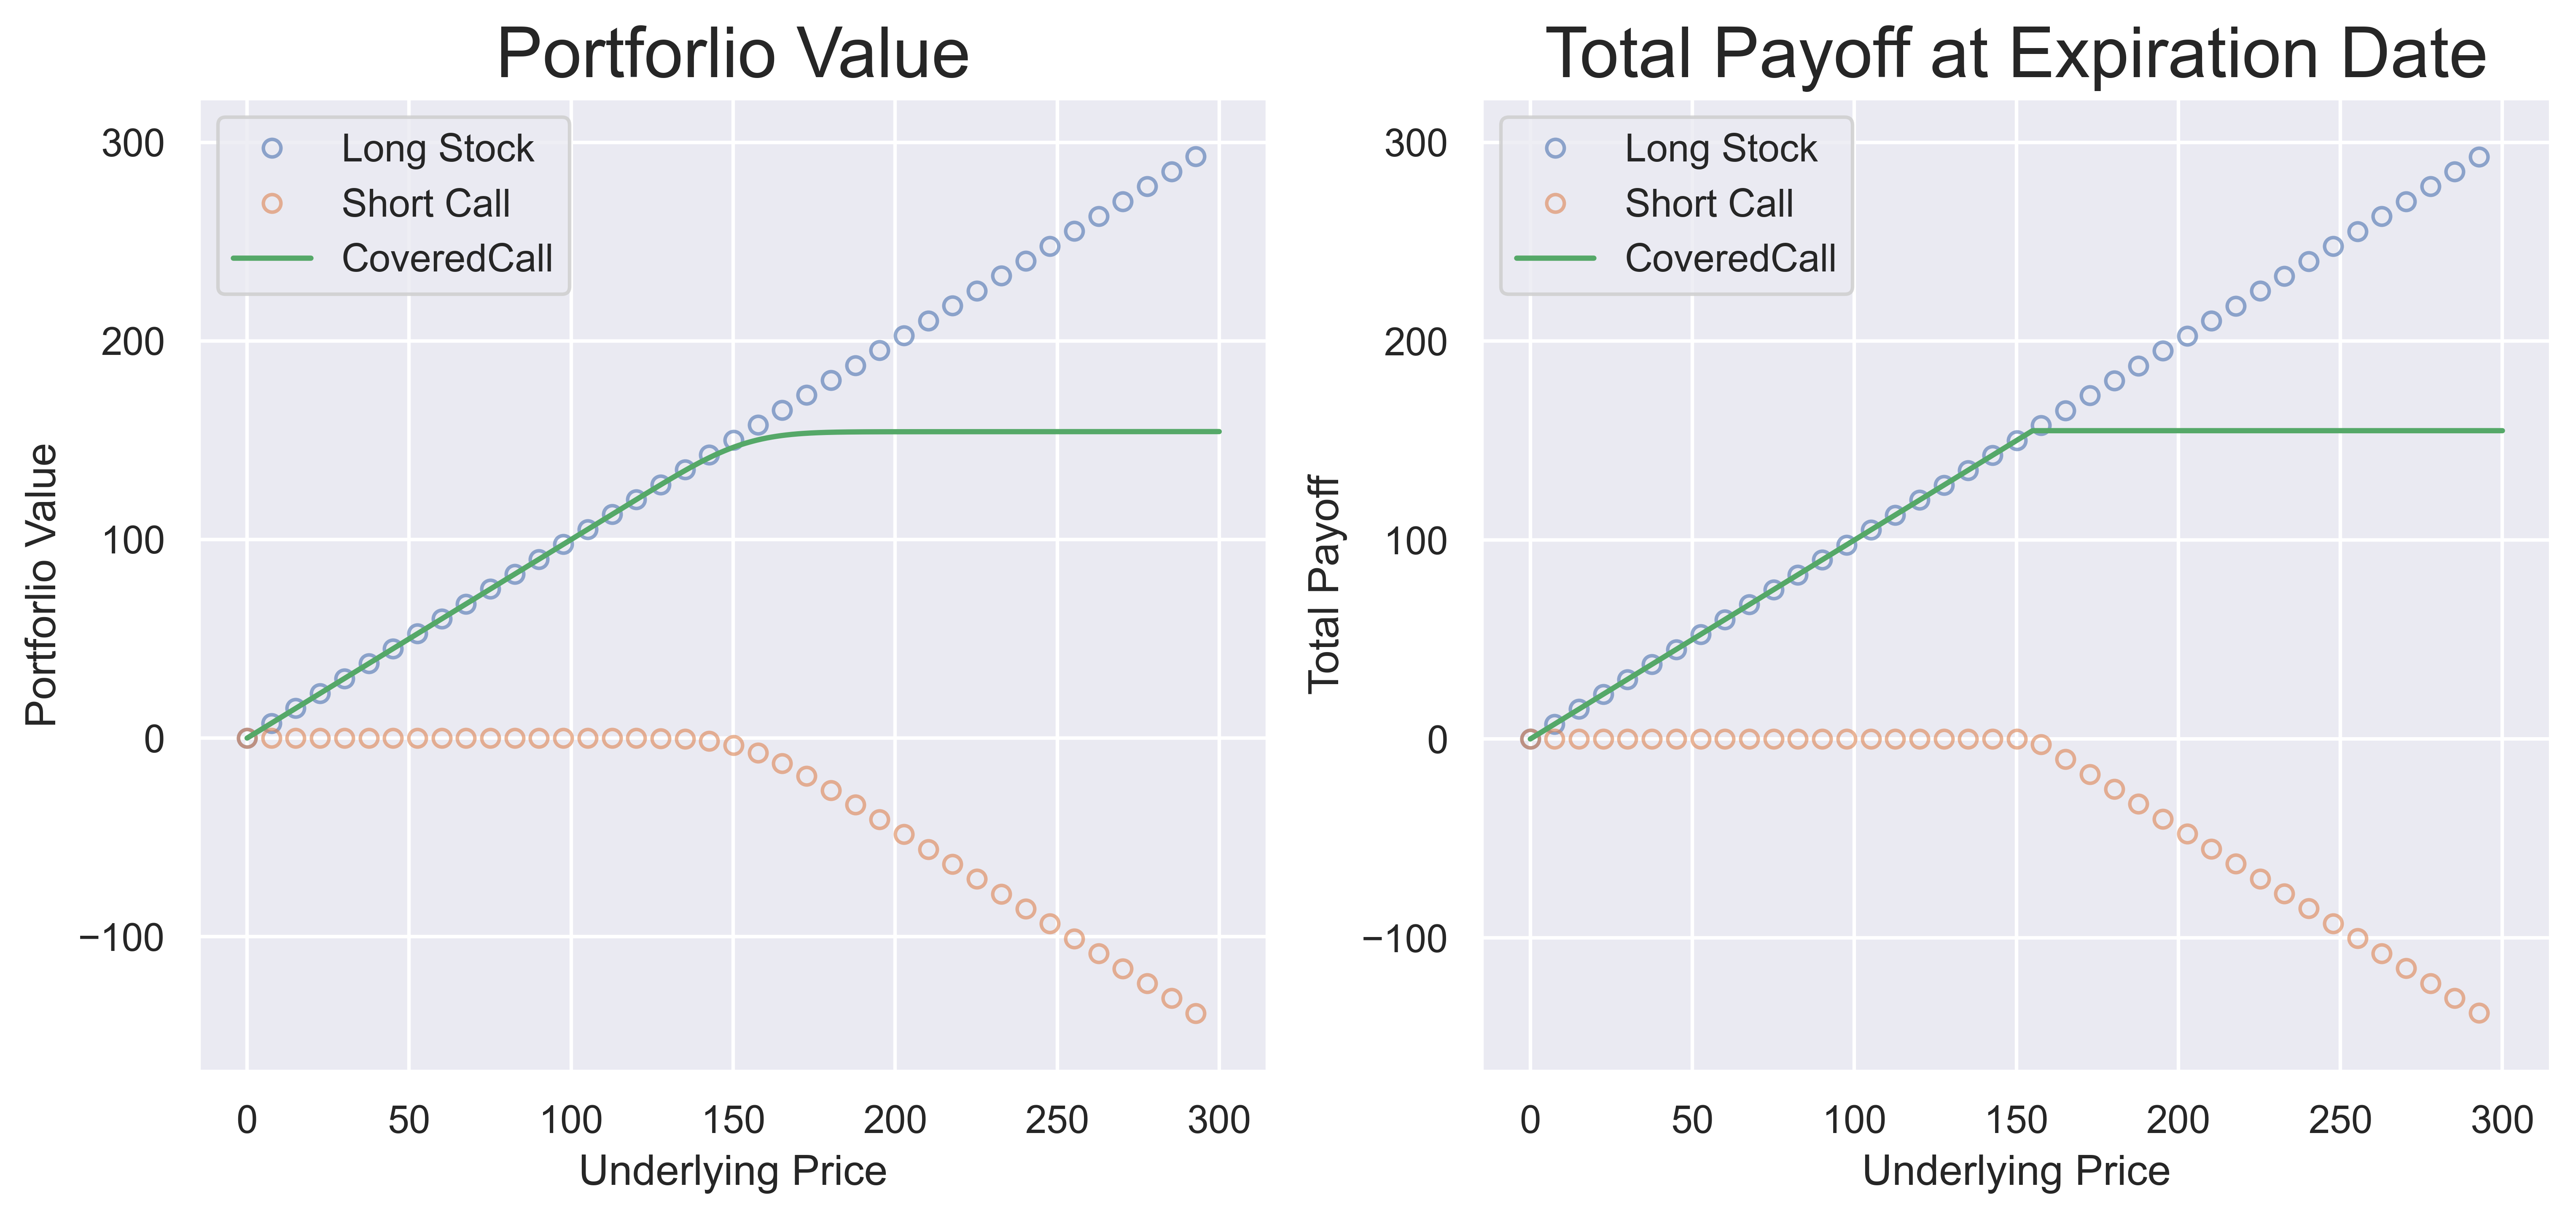
\includegraphics[width=0.75\textwidth]{./image/image_3/optionStrategy/CoveredCall.png} 
        \caption{Coverd Call}
    \end{figure}

    \item \textbf{Protective Put: Long Put + Long Stock}
    
    From the Put Call Parity, we have:
    \begin{equation}
        P + Se^{-qT} = C + Ke^{-rT}
    \end{equation}

    \textbf{Equivalent portfolio}: Long Call + $Ke^{-rT}$ Cash
    
    \textbf{Use case}: Protecting gains and mitigate risk.

    \textbf{Finding}: The value portfolio curve is much same as a Call value curve
    \begin{figure}[htbp] 
        \centering 
        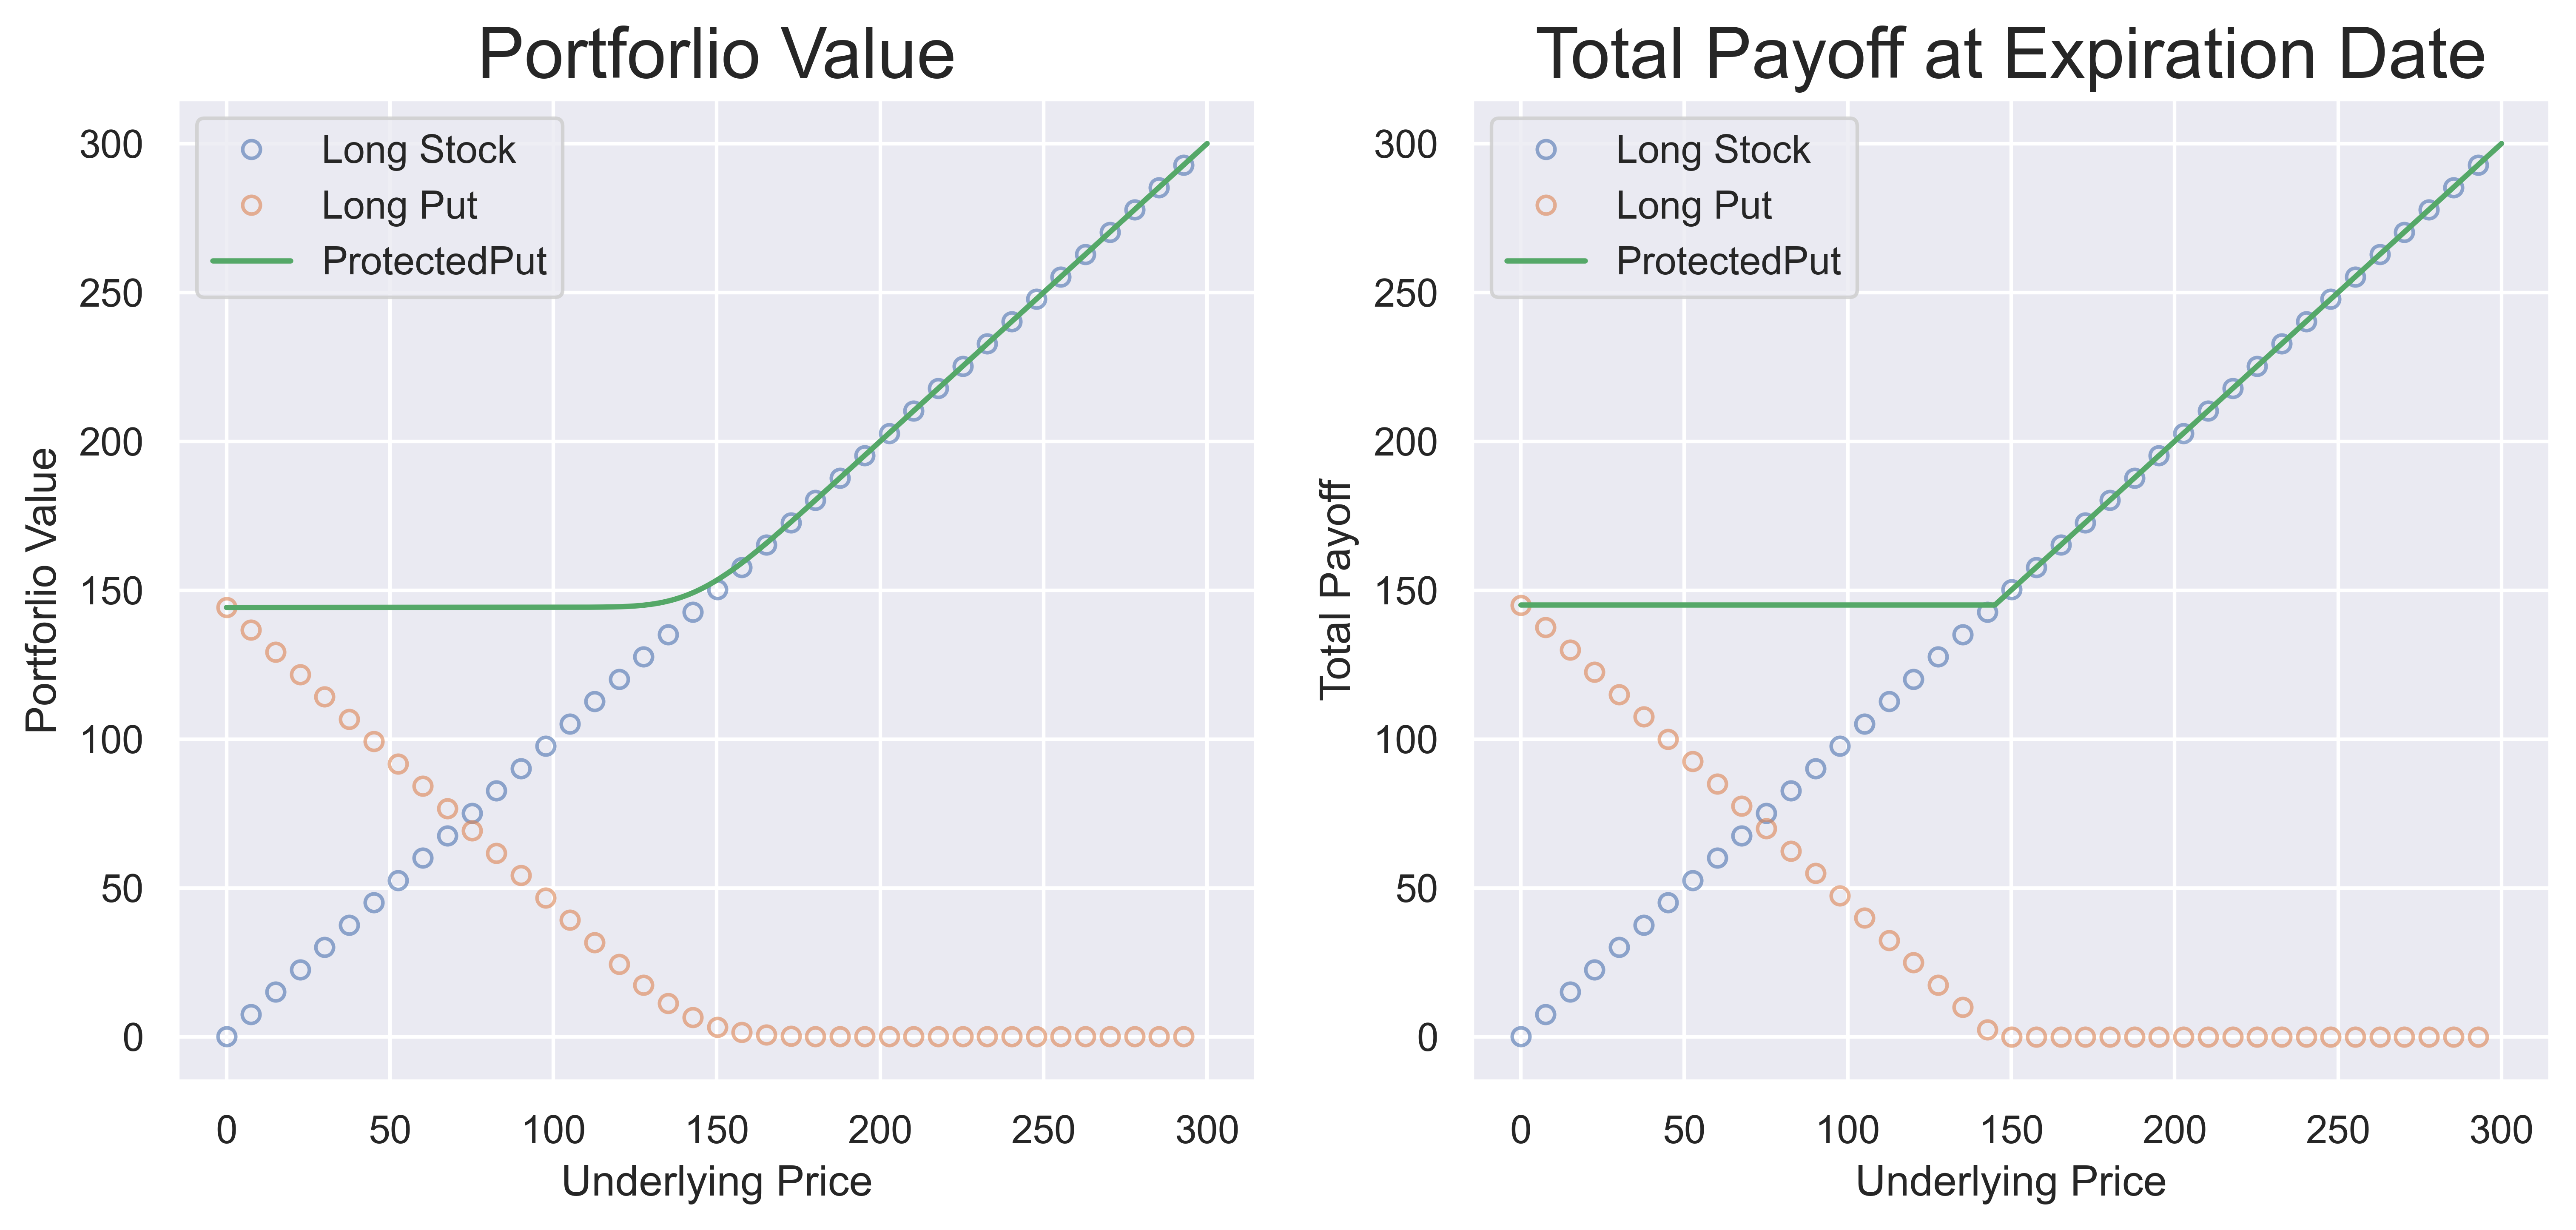
\includegraphics[width=0.75\textwidth]{./image/image_3/optionStrategy/ProtectedPut.png} 
        \caption{Protective Put}
    \end{figure}

    \item \textbf{Bull Call Spread: Long Call (Lower strike price) + Short Call (Higher strike price)}
    
    From the Put Call Parity, we have:
    \begin{equation}
        C_1 - C_2 = P_1 - P_2 + (K_2-K_1)e^{-rT}\quad (K_1 < K_2)
    \end{equation}

    \textbf{Equivalent portfolio}: Long Put ($K_1$) + Short Put($K_2$) + $(K_2-K_1)e^{-rT}$ Cash
    
    \textbf{Use case}: Expect bullish market outlook while managing risk and volatility in portfolios.

    \textbf{Finding}: The strategy limit the loss and profit.
    \begin{figure}[htbp] 
        \centering 
        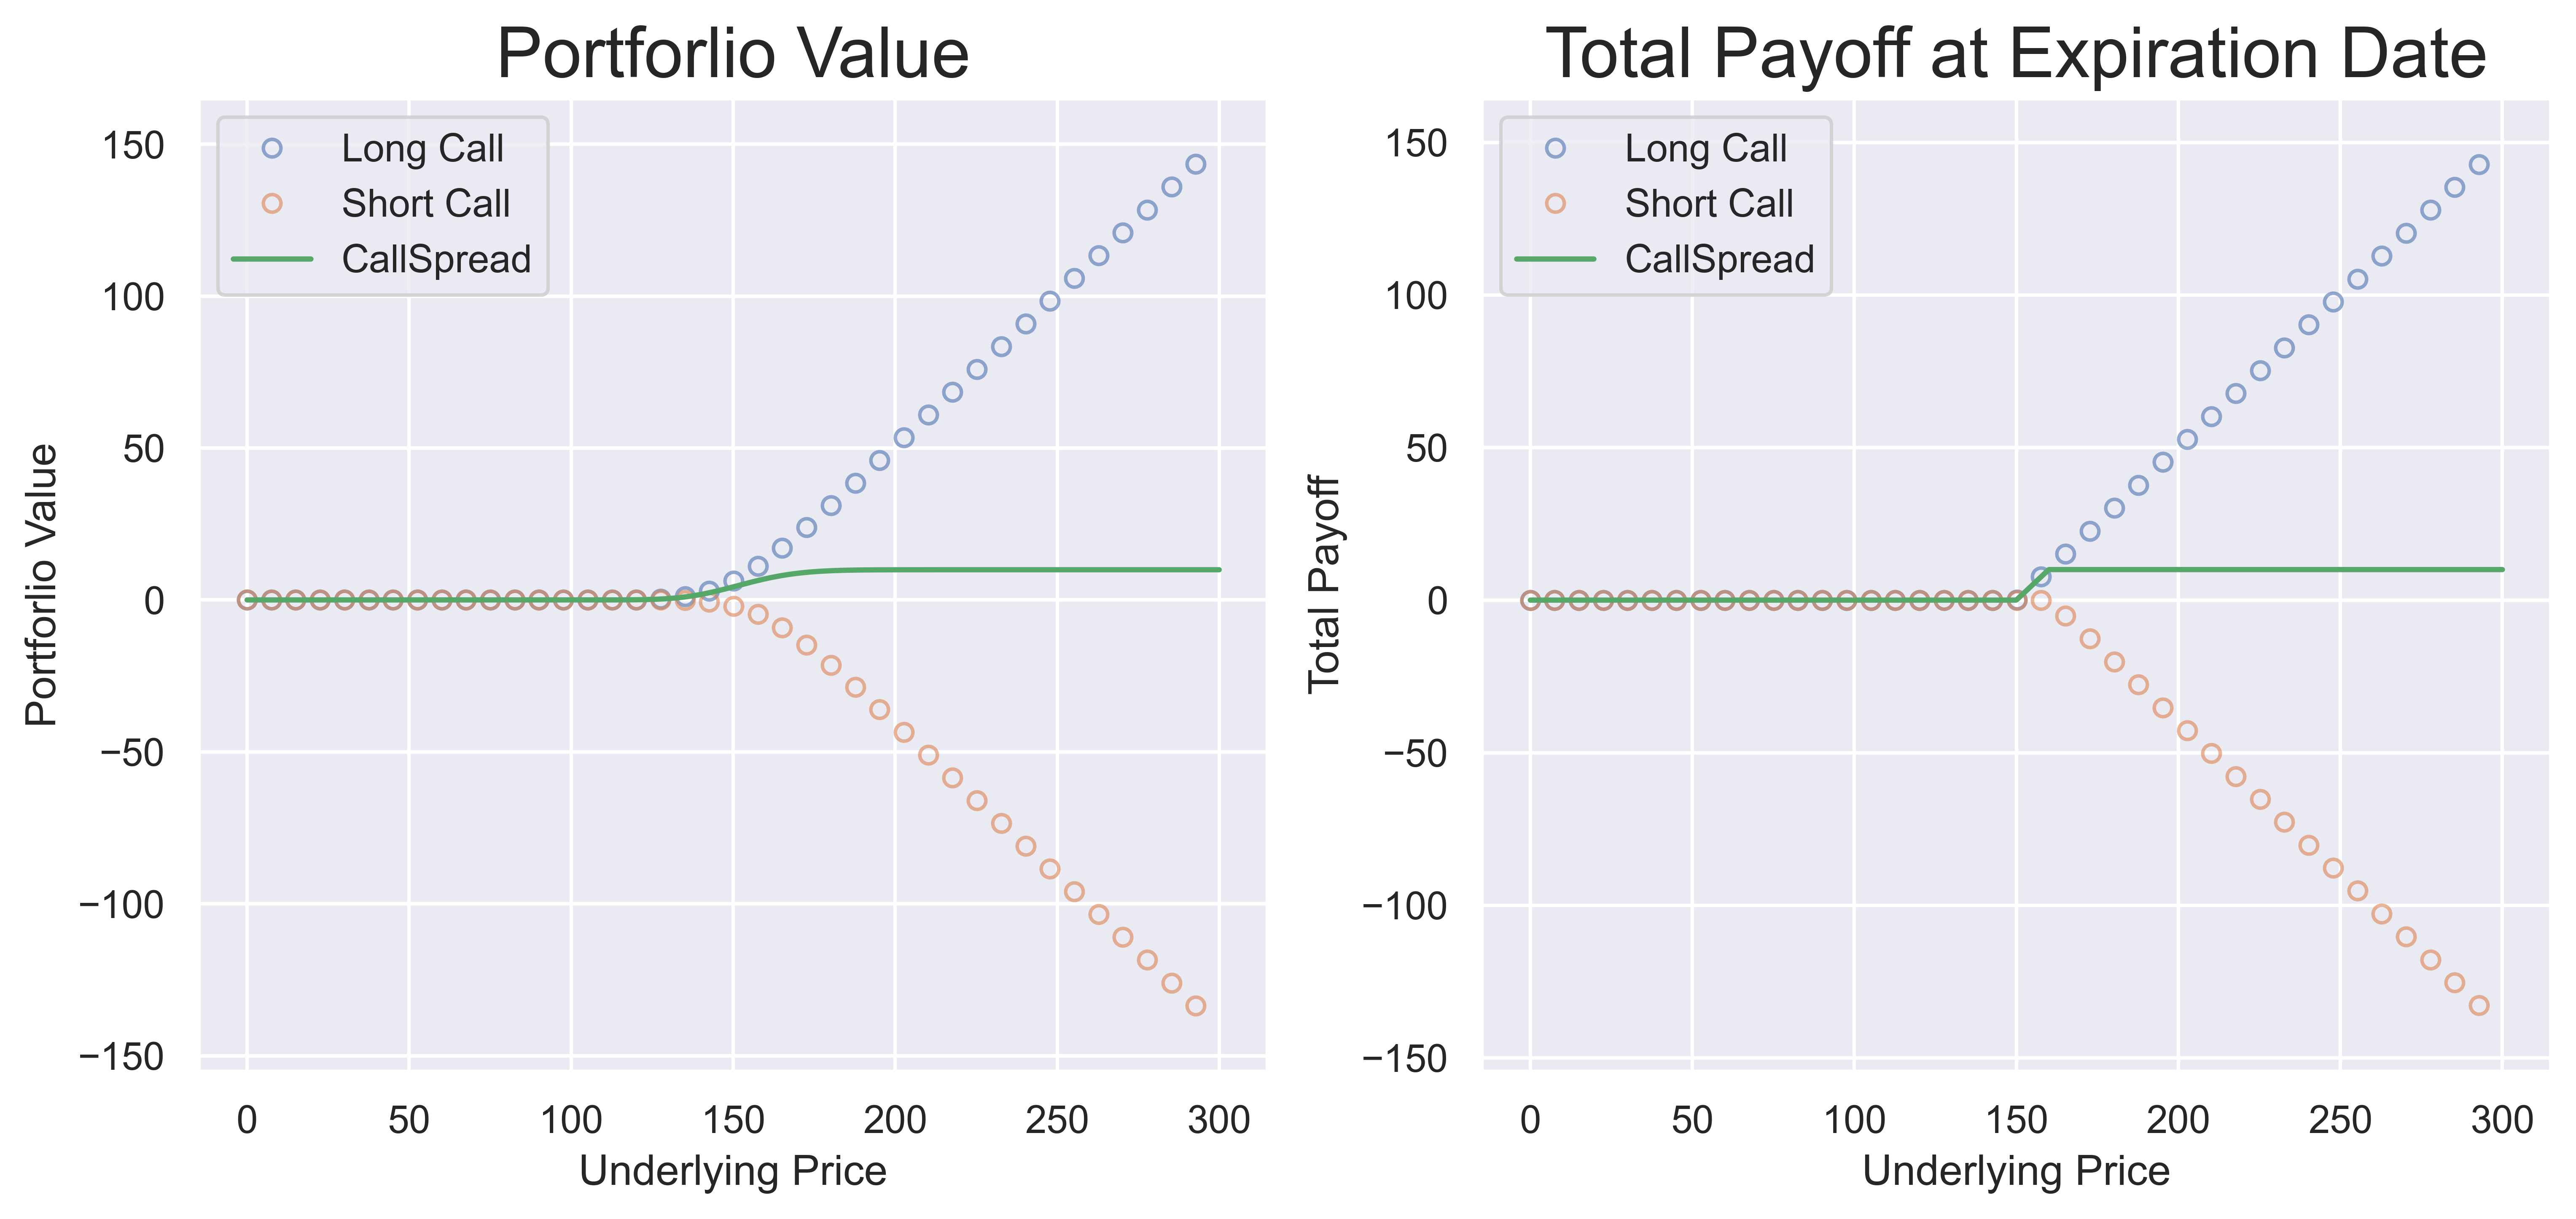
\includegraphics[width=0.75\textwidth]{./image/image_3/optionStrategy/CallSpread.png} 
        \caption{Bull Call Spread}
    \end{figure}
    
    \item \textbf{Bear Put Spread: Long Put (Higher strike price) + Short Put (Lower strike price)}
    
    From the Put Call Parity, we have:
    \begin{equation}
        P_1 - P_2 =  C_1 - C_2+ (K_1-K_2)e^{-rT}\quad (K_1 > K_2)
    \end{equation}

    \textbf{Equivalent portfolio}: Long Call ($K_1$) + Short Call($K_2$) + $(K_1-K_2)e^{-rT}$ Cash
    
    \textbf{Use case}: Expect bearish market outlook while managing risk and volatility in portfolios.

    \textbf{Finding}: The strategy limit the loss and profit.
    \begin{figure}[htbp] 
        \centering 
        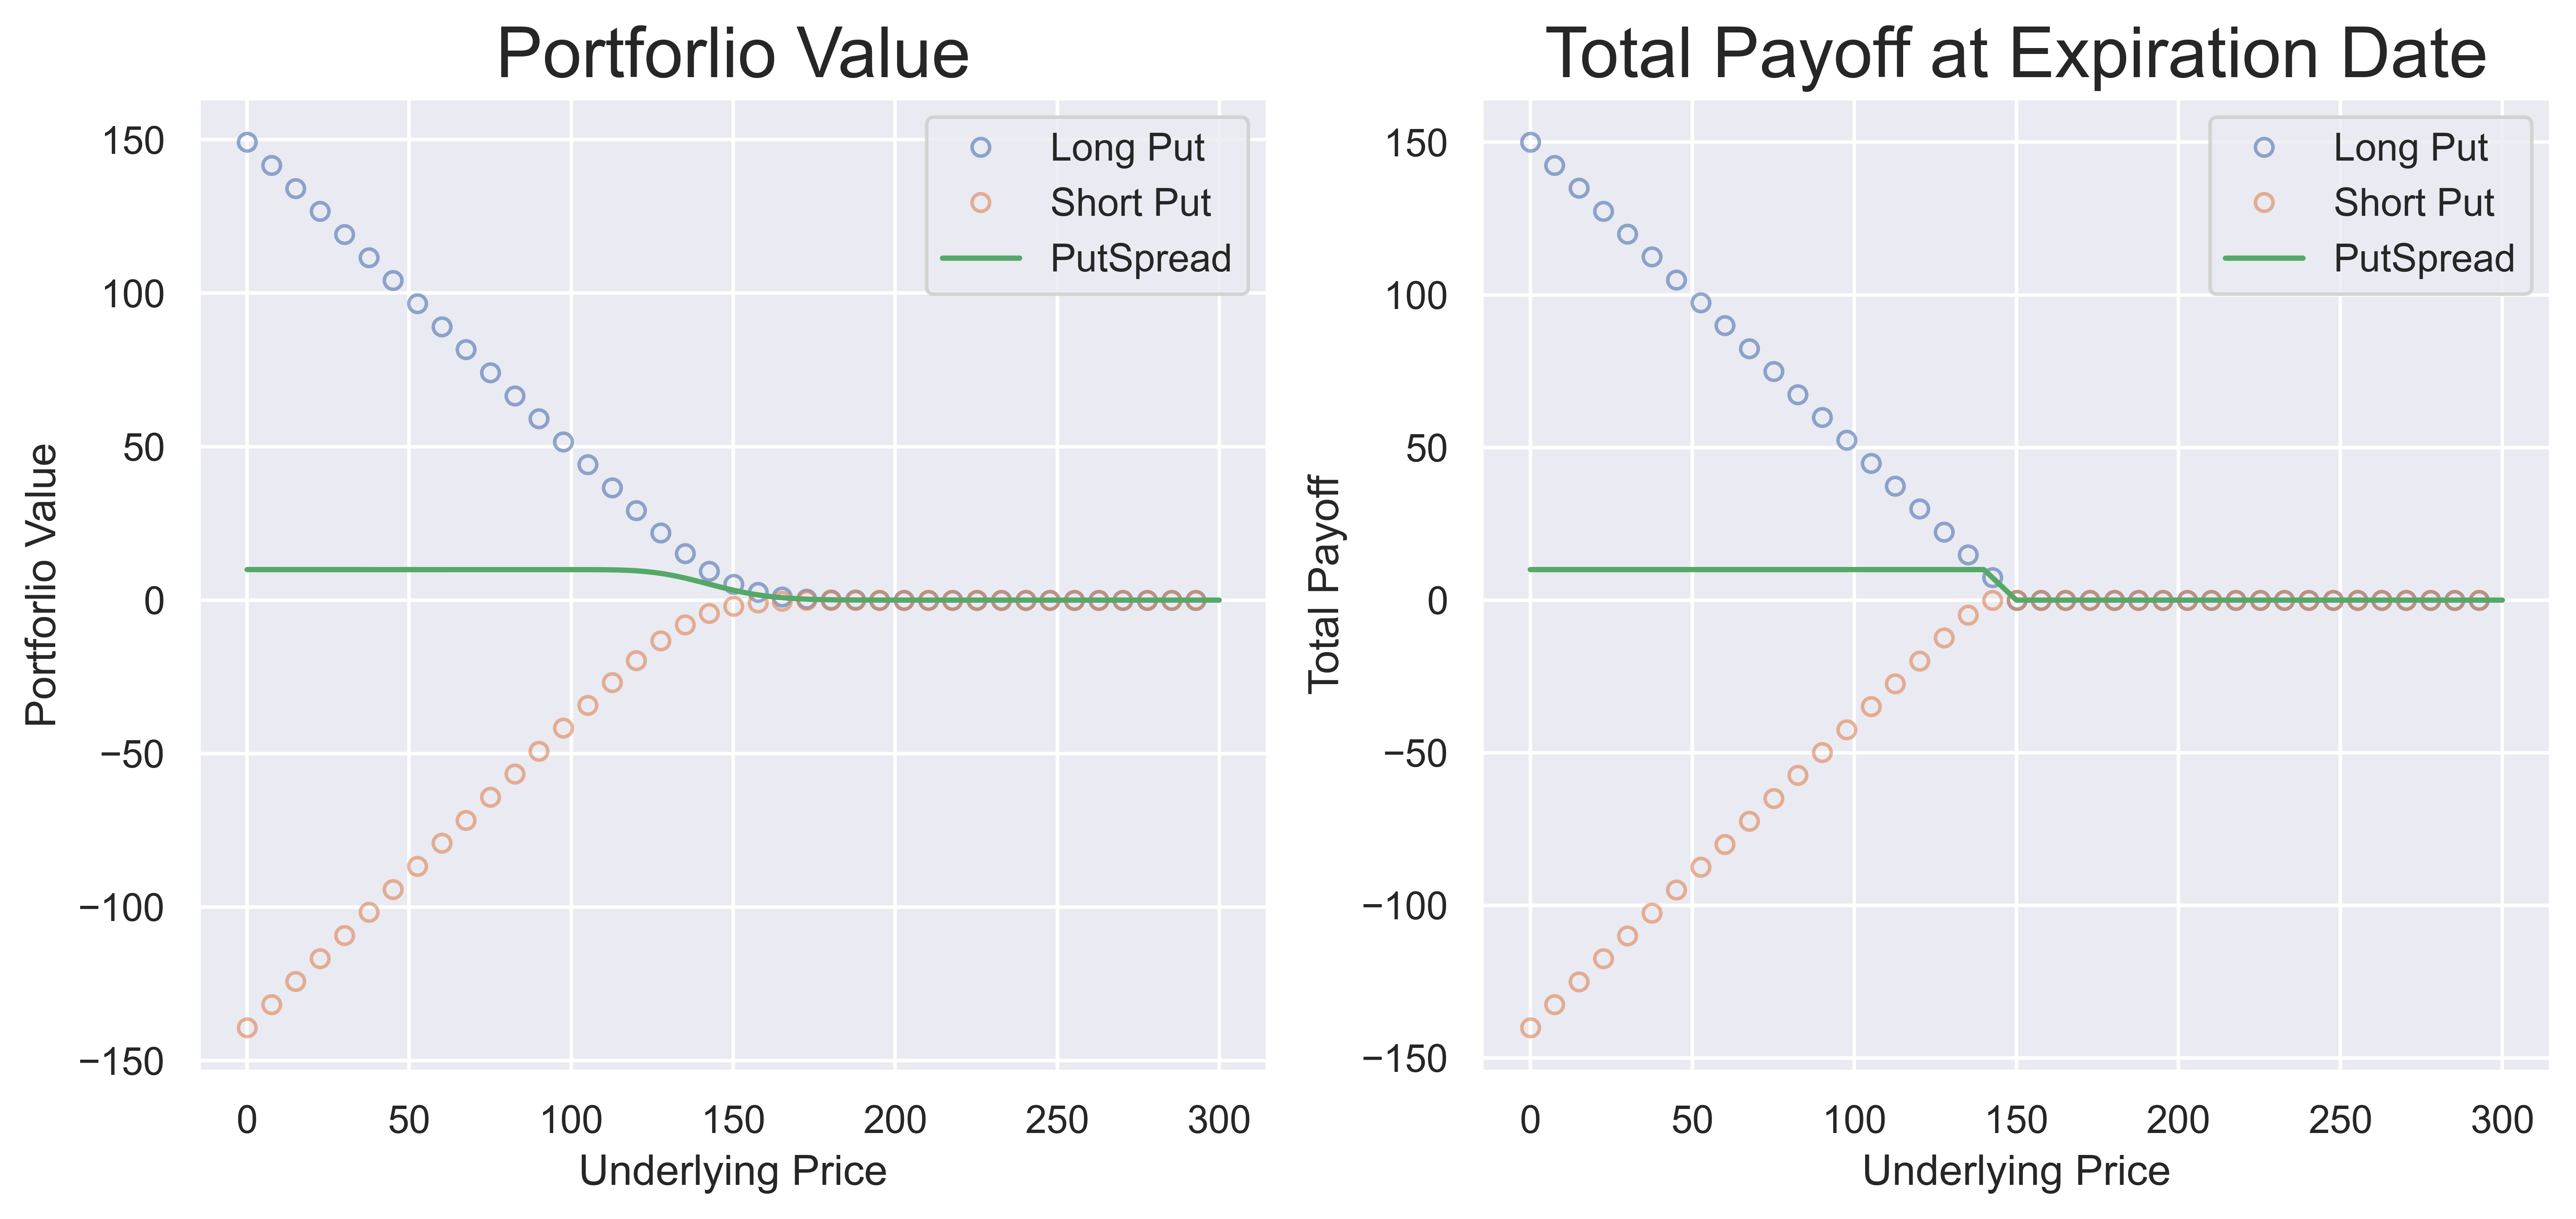
\includegraphics[width=0.75\textwidth]{./image/image_3/optionStrategy/PutSpread.png} 
        \caption{Bear Put Spread}
    \end{figure}

    \item \textbf{Straddle: Long Call + Long Put}
    
    From the Put Call Parity, we have:
    \begin{equation}
        C + P = 2P + Se^{-qT} - Ke^{-rT} = 2C + Ke^{-rT} - Se^{-qT}
    \end{equation}

    \textbf{Equivalent portfolio}: 
    \begin{enumerate}
        \item 2 units of Long Call + Long Stock + Borrow $Ke^{-rT}$ Cash
        \item 2 units of Long Put + Short Stock +  $Ke^{-rT}$ Cash
    \end{enumerate}
    
    \textbf{Use case}: Expect significant price movements in an underlying asset while managing risk and uncertainty in their portfolios.

    \textbf{Finding}: Only large price movements could make profits. Otherwise, we would lose money used to cost to build such strategy.
    \begin{figure}[htbp] 
        \centering 
        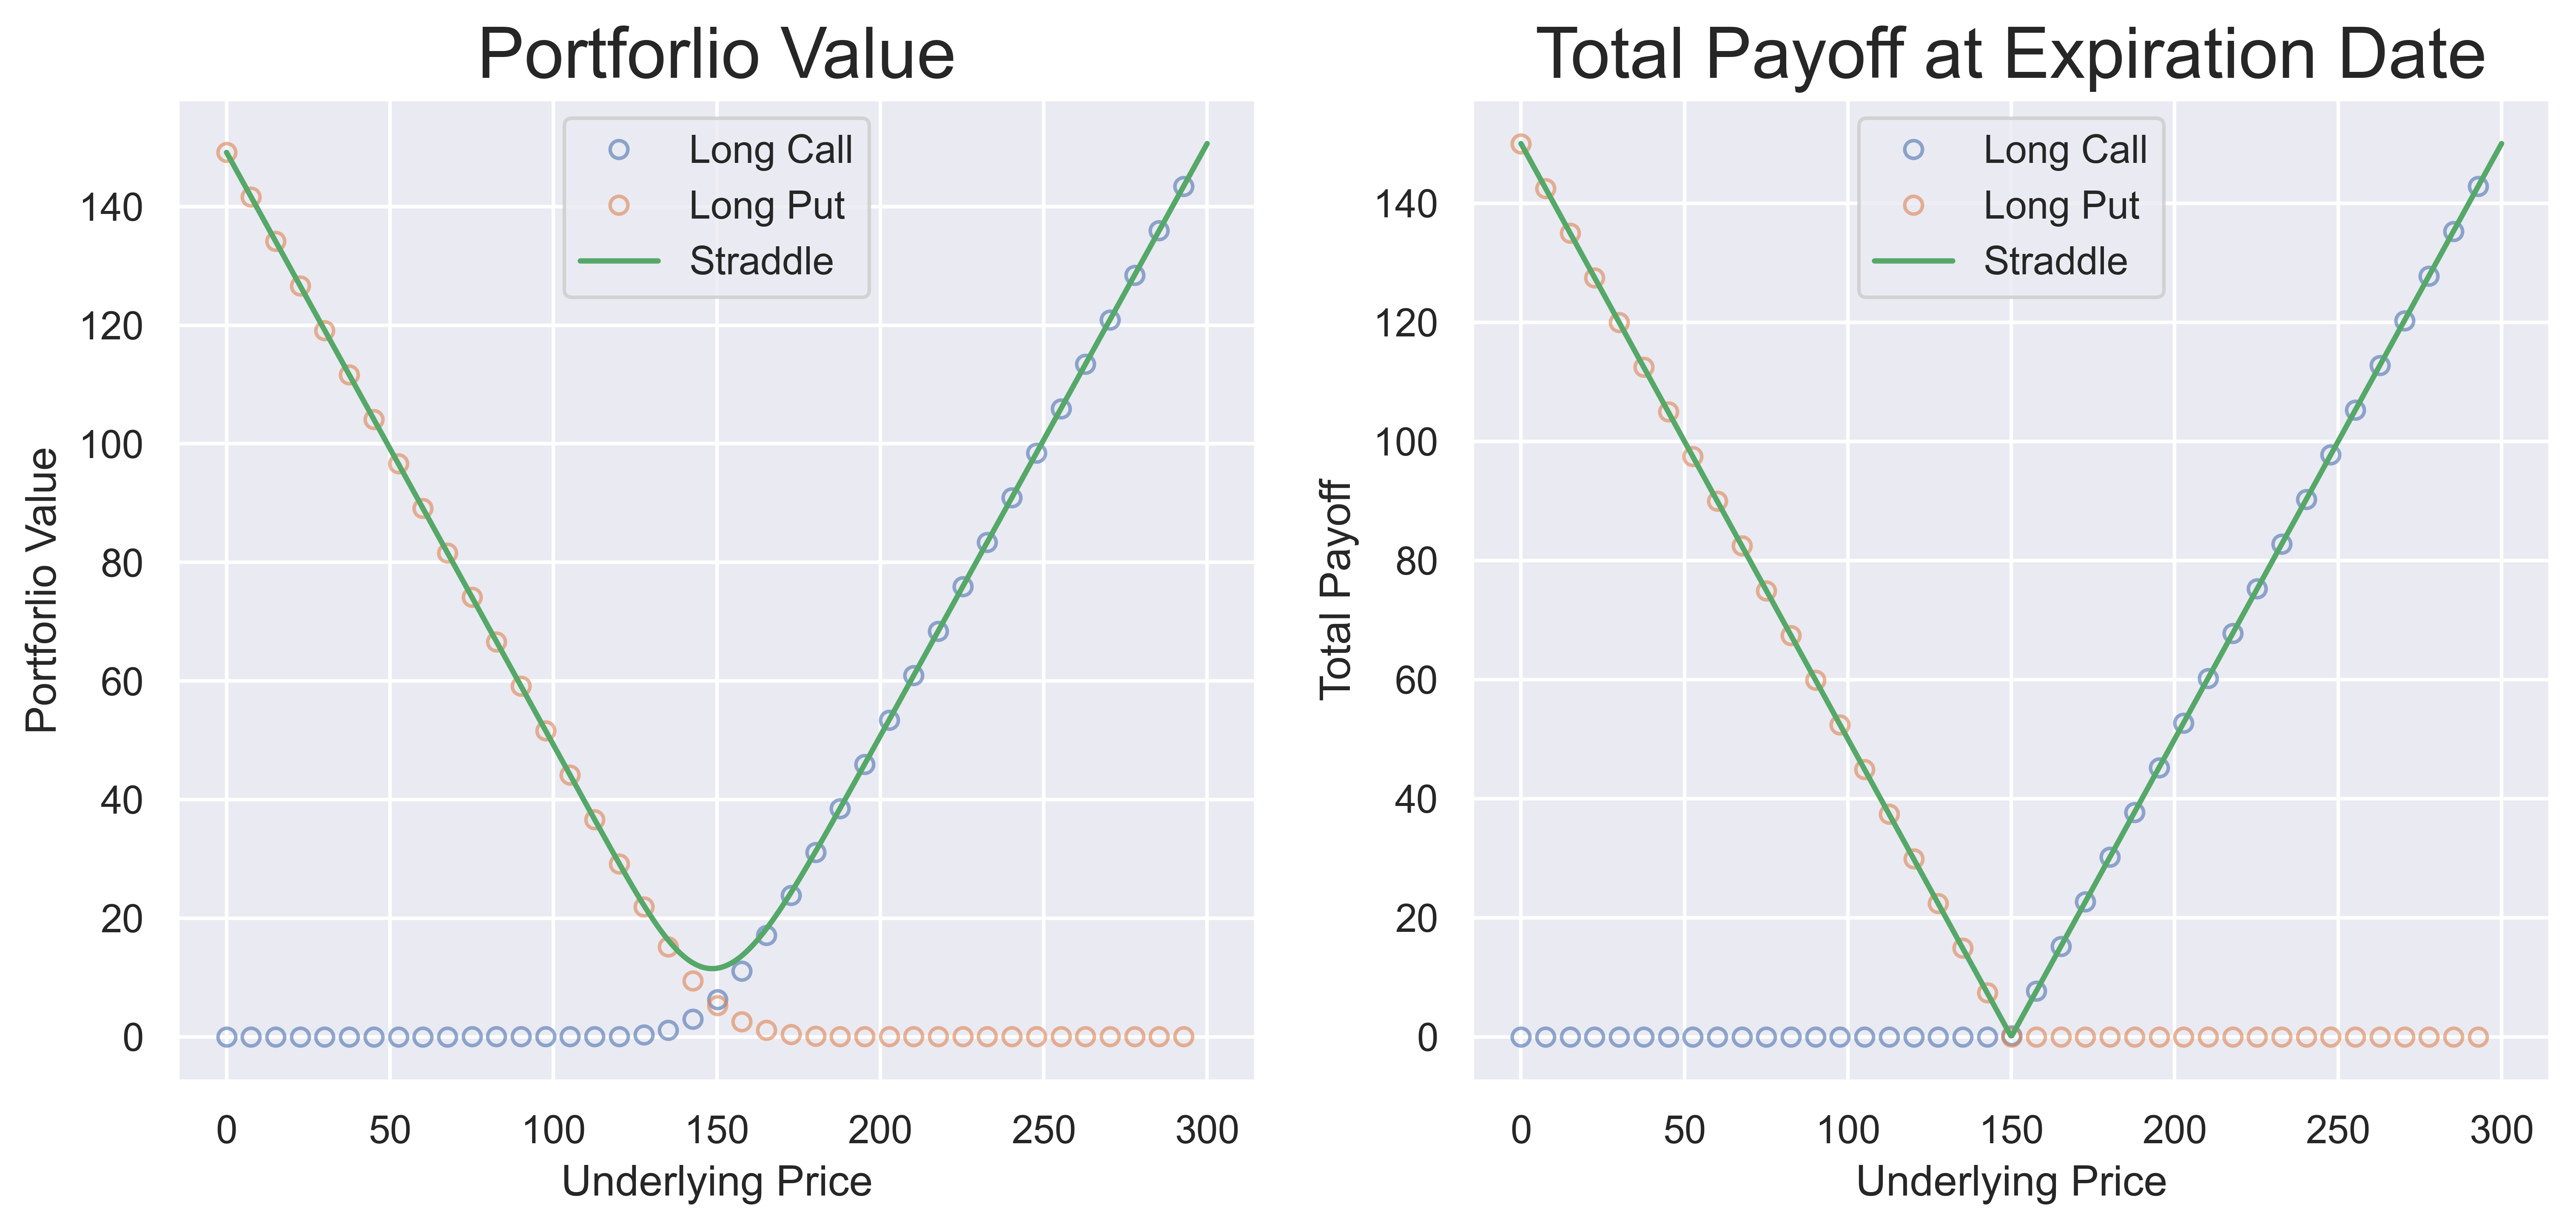
\includegraphics[width=0.75\textwidth]{./image/image_3/optionStrategy/Straddle.png} 
        \caption{Straddle}
    \end{figure}

    \newpage

    \item \textbf{Synthetic Long Call: Long Call + Short Put}
    
    From the Put Call Parity, we have:
    \begin{equation}
        C - P = Se^{-qT} - Ke^{-rT}
    \end{equation}

    \textbf{Equivalent portfolio}: Long Stock + Borrow $Ke^{-rT}$ Cash
    
    \textbf{Use case}: Mimic a long call option, lower costs, hedge against downside risk, and manage risk in portfolios. 

    \textbf{Finding}: Such strategy value is much same as stock future.
    \begin{figure}[htbp] 
        \centering 
        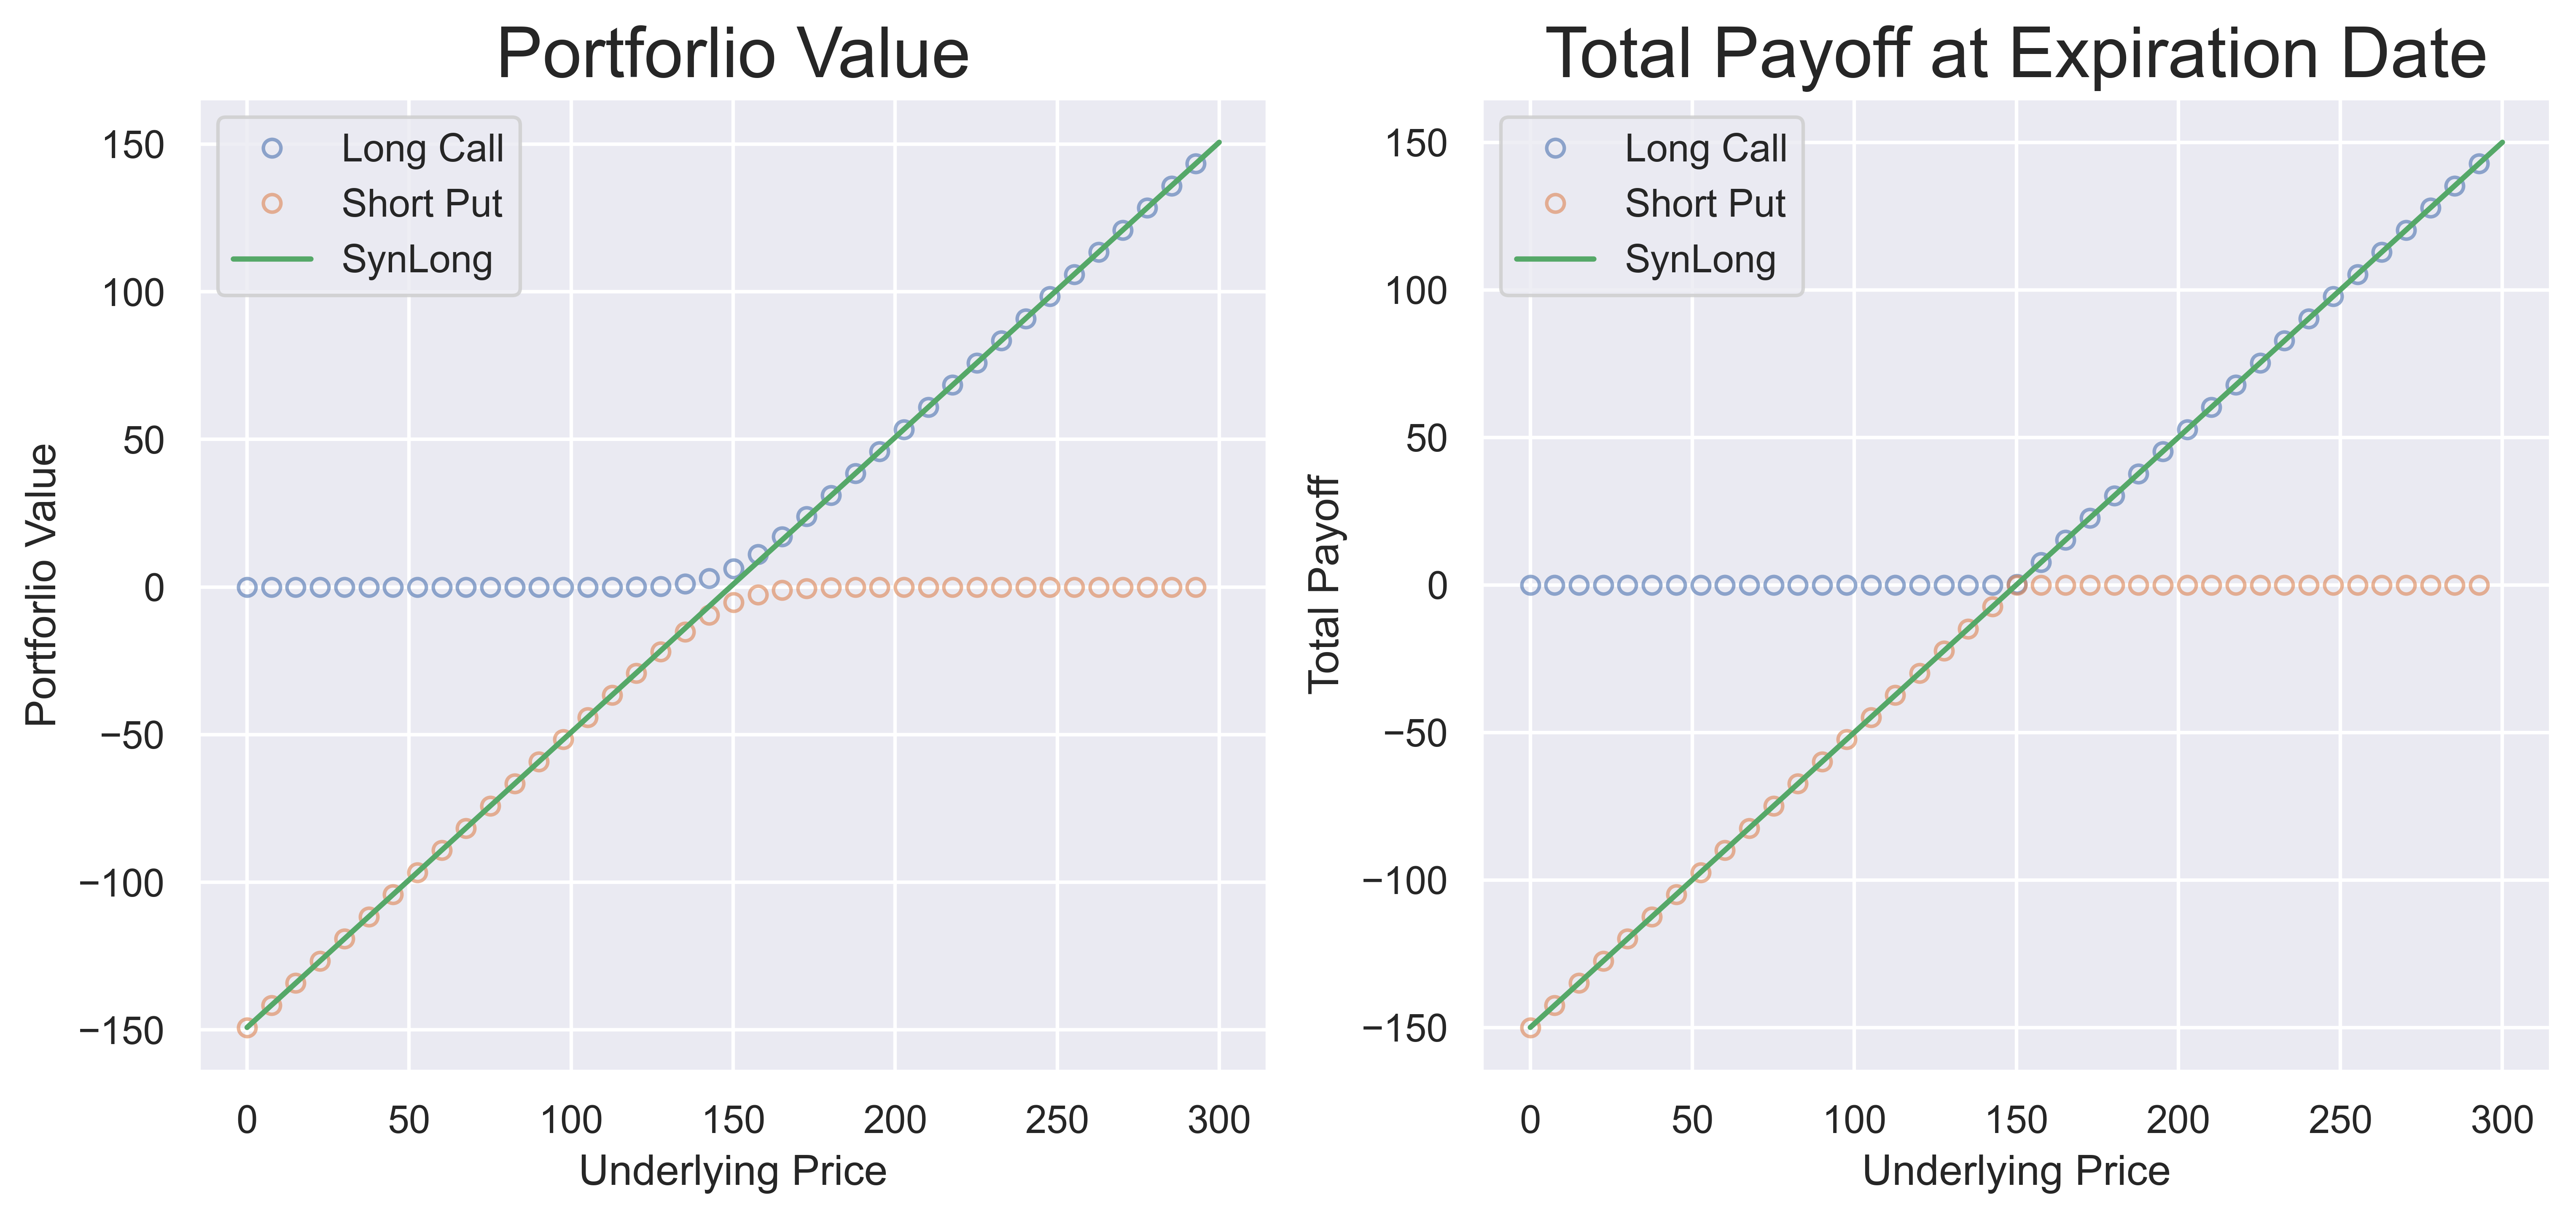
\includegraphics[width=0.75\textwidth]{./image/image_3/optionStrategy/SynLong.png} 
        \caption{Synthetic Long Call}
    \end{figure}
    

    \item \textbf{Call}

    From the Put Call Parity, we have:
    \begin{equation}
        C  = P + Se^{-qT} - Ke^{-rT}
    \end{equation}

    \textbf{Equivalent portfolio}: Long Put + Long Stock + Borrow $Ke^{-rT}$ Cash
    
    \textbf{Use case}: Looking to speculate on price increases, hedge against downside risk, lower costs, and generate income in their portfolios.

    \textbf{Finding}: It could help us amplify the return at a certain cost.
    \begin{figure}[htbp] 
        \centering 
        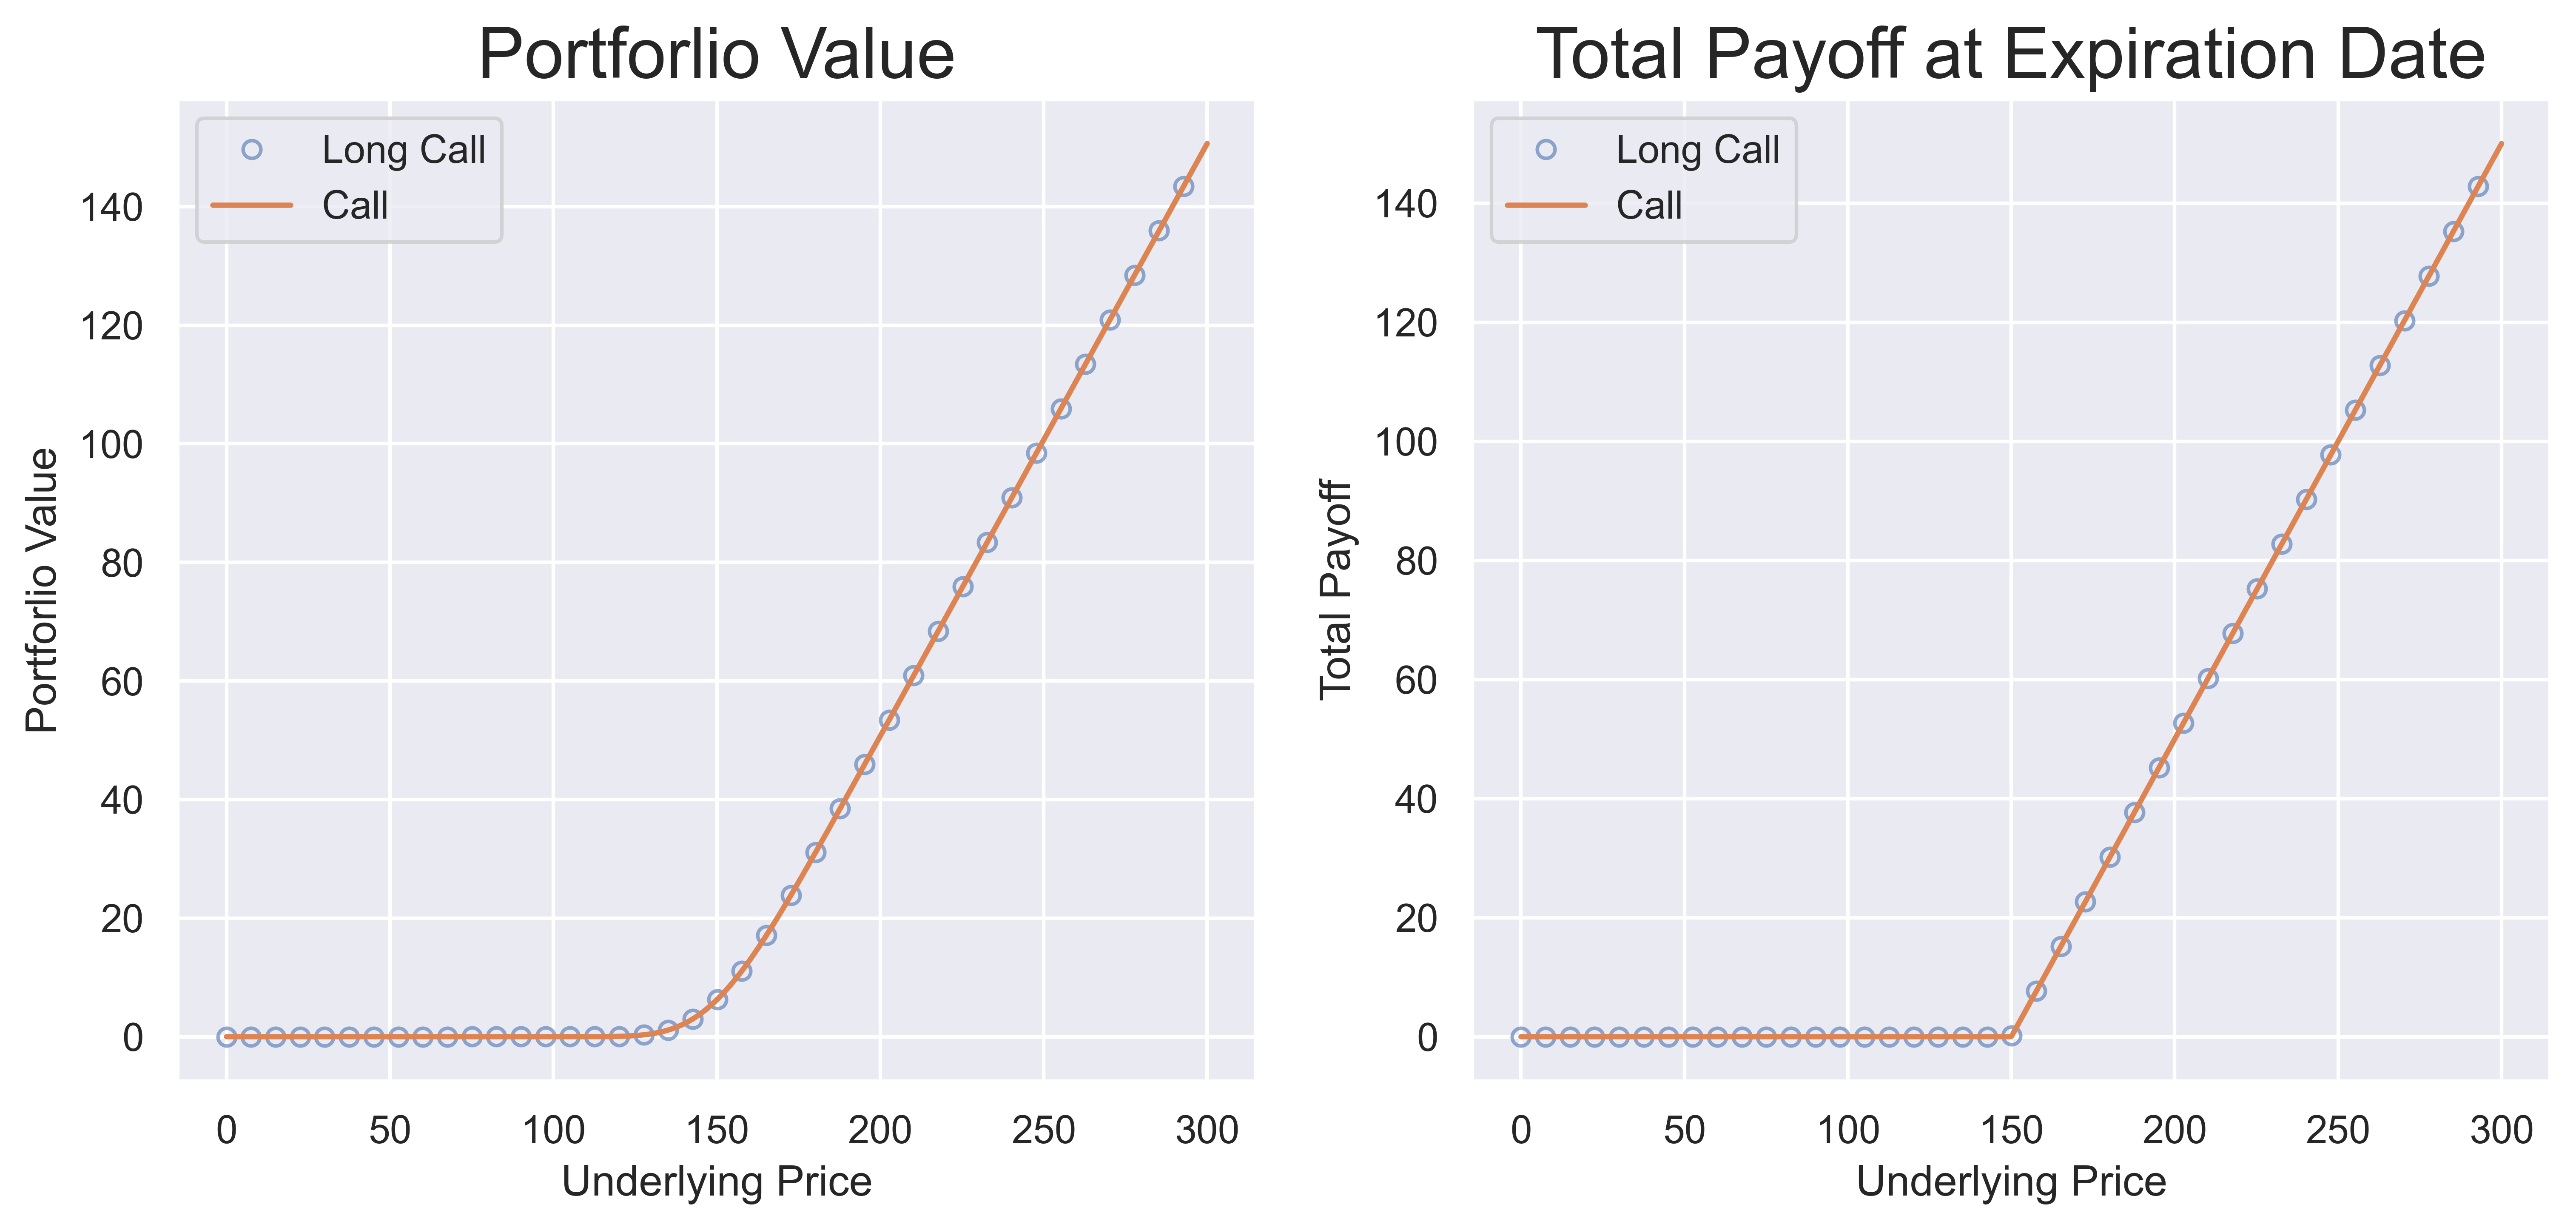
\includegraphics[width=0.75\textwidth]{./image/image_3/optionStrategy/Call.png} 
        \caption{Call}
    \end{figure}

    \item \textbf{Put}

    From the Put Call Parity, we have:
    \begin{equation}
        P = C - Se^{-qT} + Ke^{-rT}
    \end{equation}

    \textbf{Equivalent portfolio}: Long Call + Short Stock + $Ke^{-rT}$ Cash
    
    \textbf{Use case}: Looking to speculate on price decreases, hedge against upside risk, lower costs, and generate income in portfolios. 

    \textbf{Finding}: It could help us amplify the return at a certain cost.
    \begin{figure}[htbp] 
        \centering 
        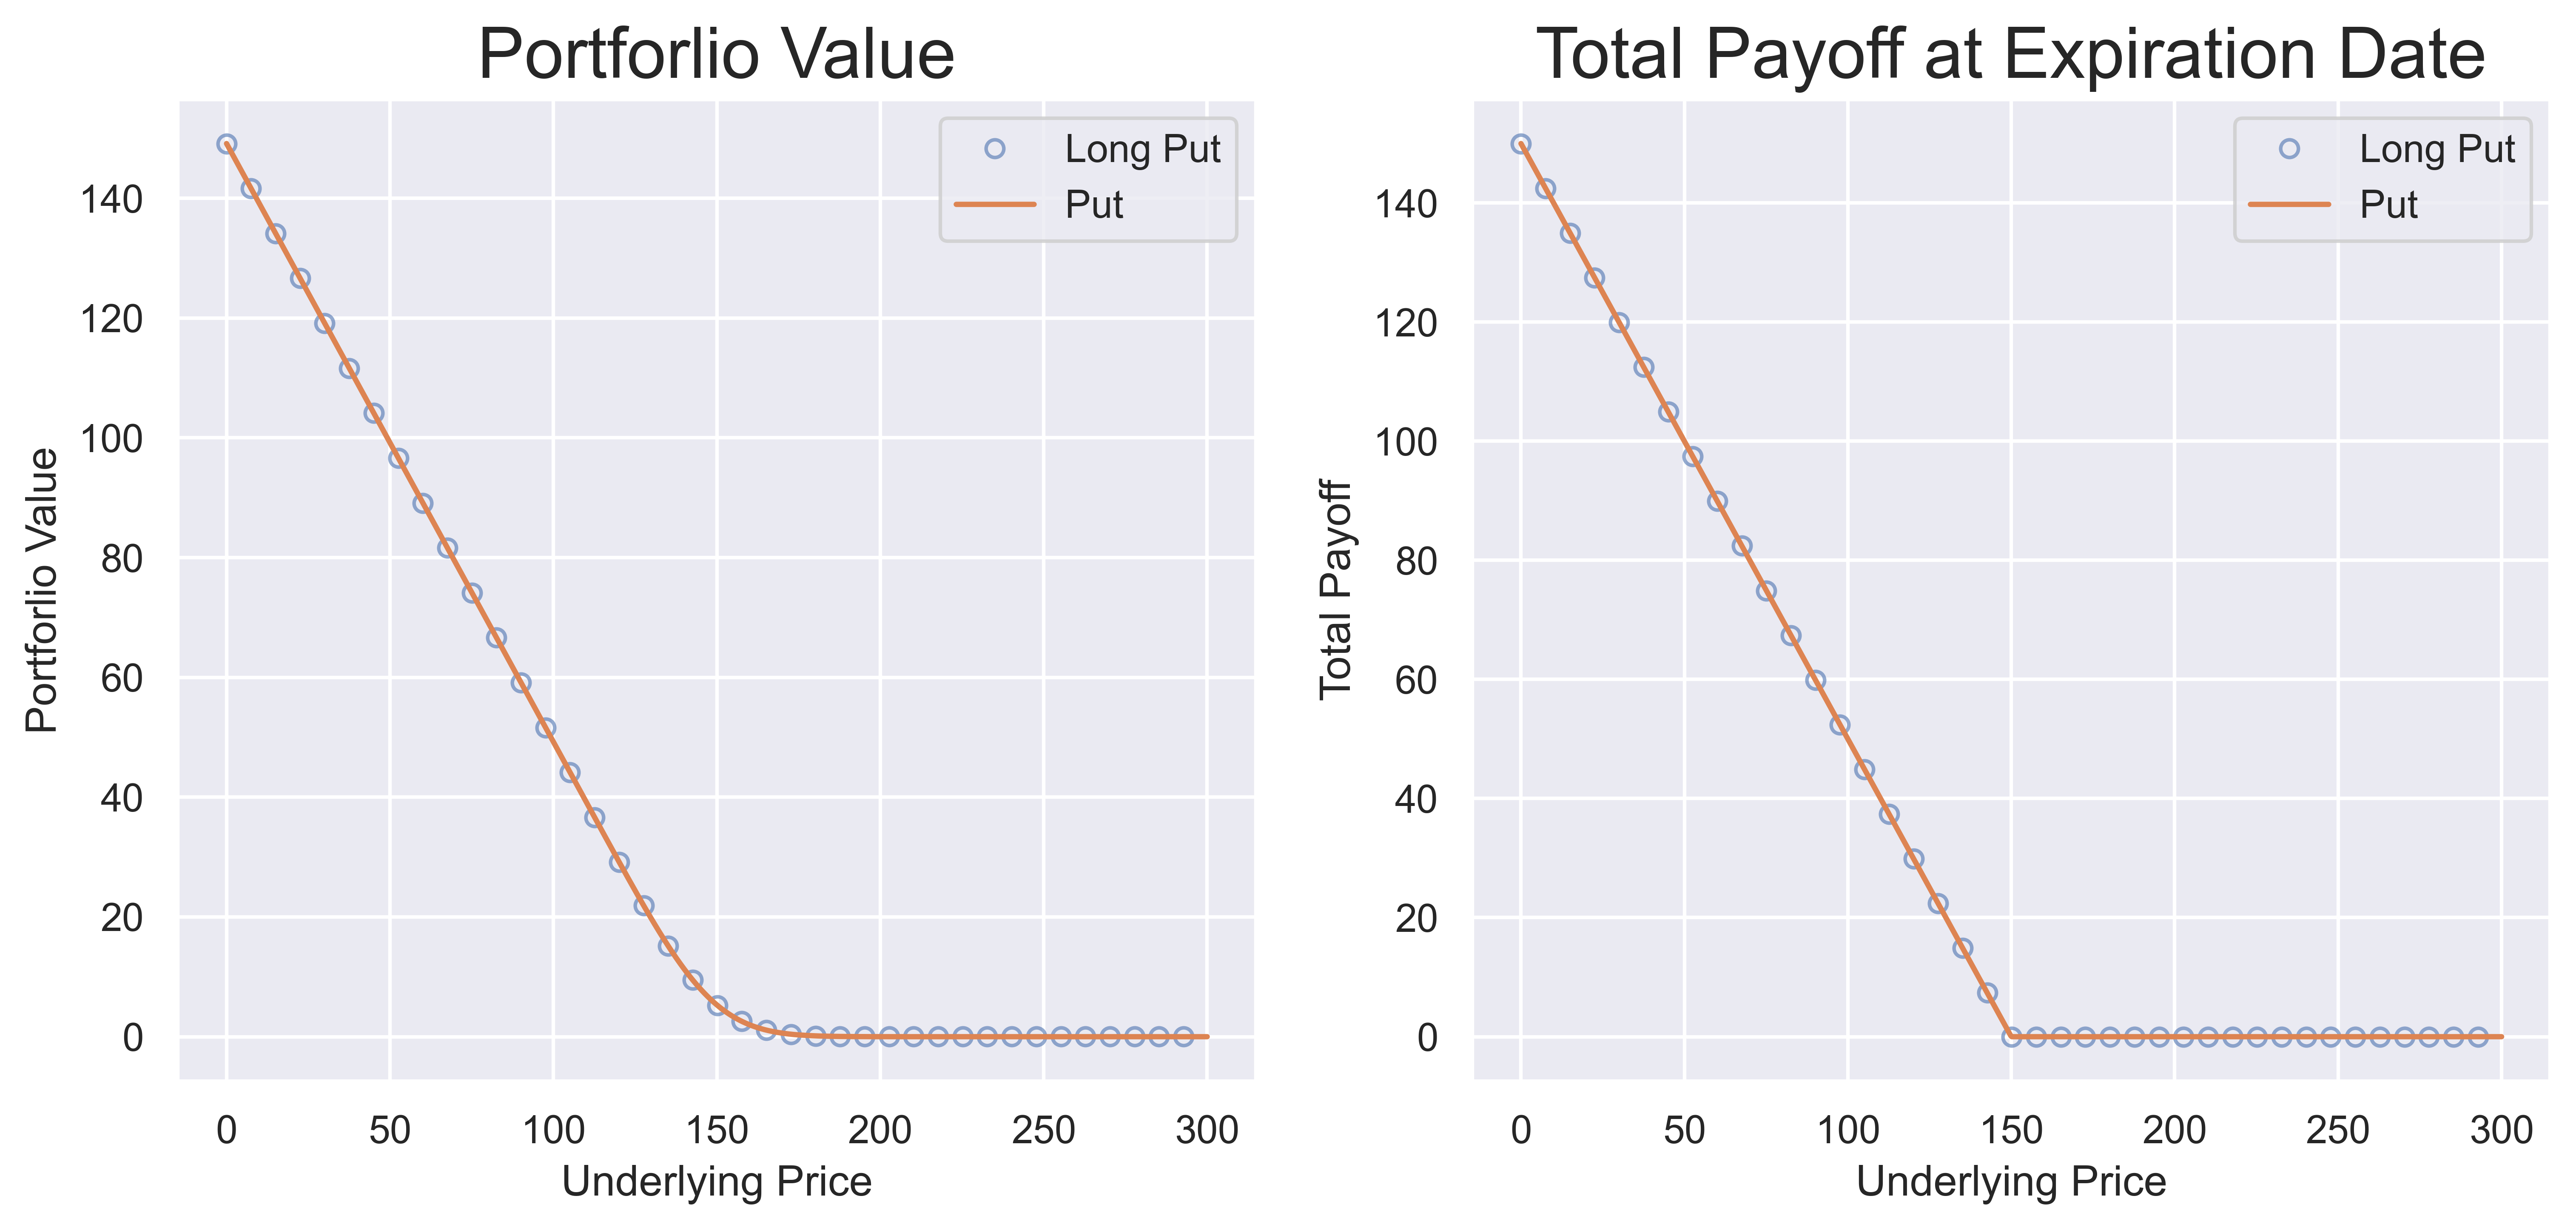
\includegraphics[width=0.75\textwidth]{./image/image_3/optionStrategy/Put.png} 
        \caption{Put}
    \end{figure}

    \newpage

    \item \textbf{Stock}
    \begin{figure}[htbp] 
        \centering 
        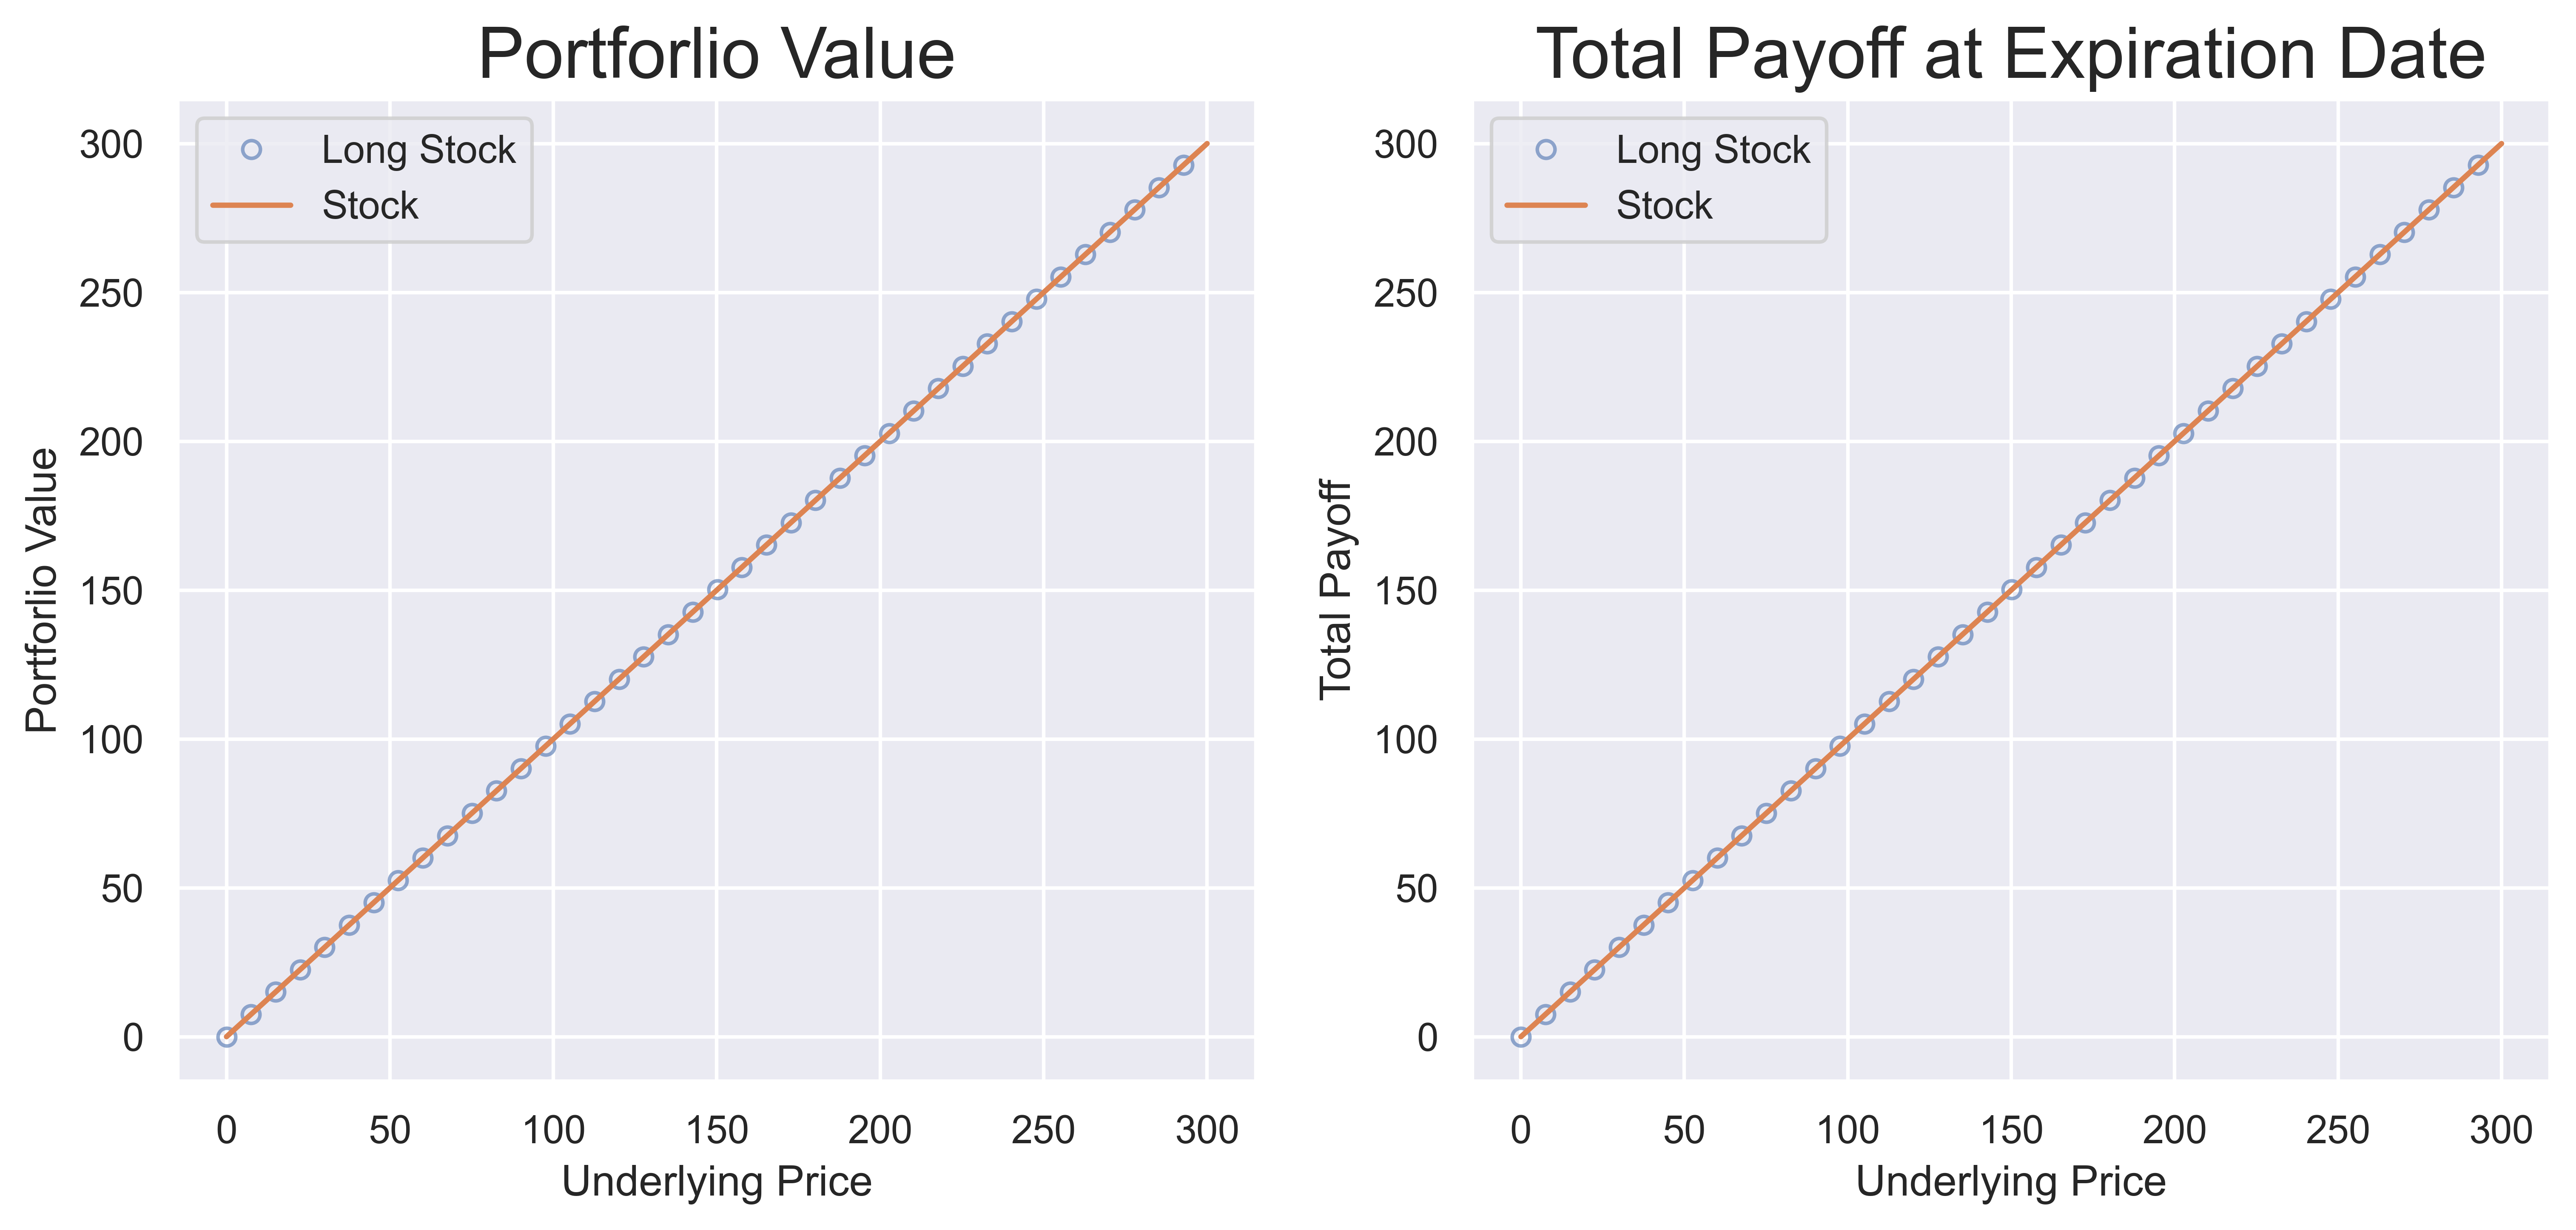
\includegraphics[width=0.75\textwidth]{./image/image_3/optionStrategy/Stock.png} 
        \caption{Stock}
    \end{figure}

\end{enumerate}

\subsection*{\textcolor{orange}{Simulation \& Risk Metrics}}

We use AR(1) model to fit the return of AAPL and simulate 10 days ahead. Apply those simulated returns 100000 times, to the current price, assume the implied volatility holds ten days later and use generalized Black-Scholes model to calculate the optoin price and corresponding portfolio value.

Based on those values, we calculate the mean, value at risk and expected shortfall of those portfolio vaiation. We have the following chart:



\begin{table}[htbp]
    \centering
    \caption{Simulated Portfolio Value 10 Days Later}
    \begin{tabular}{@{}ccccc@{}}
        \toprule
        \textbf{Portfolio} & \textbf{Mean(Portfolio Value)} & \textbf{Mean(Variation)} & \textbf{VaR} & \textbf{ES}\\
        \midrule
        Straddle     &             13.236627 &     1.586627 &   1.378317 &   1.387136 \\
        SynLong      &              2.050838 &     0.100838 &   16.24976 &  19.975054 \\
        CallSpread   &              4.519231 &    -0.070769 &    3.89146 &   4.181353 \\
        PutSpread    &              3.292349 &     0.282349 &     2.6562 &   2.811006 \\
        Stock        &            151.334622 &     0.304622 &  16.007244 &  19.710478 \\
        Call         &              7.643733 &     0.843733 &   6.039037 &   6.362422 \\
        Put          &              5.592895 &     0.742895 &   4.401389 &   4.601255 \\
        CoveredCall  &            146.323396 &    -0.656604 &  12.191148 &  15.780425 \\
        ProtectedPut &            154.976053 &     0.936053 &   8.074428 &   8.681969 \\
        \bottomrule
    \end{tabular}
\end{table}

    
As we can see, Synthetic Long Call and Stock have the most VaR and ES, which means they have higher risk exposure than others. The Straddle and PutSpread are the most conservative portfolios. From the above data, we could sort the portfolios based on their risk exposure:

\textbf{Synthetic Long Call > Stock > Covered Call > Protected Put > Call > Put > Call Spread > Put Spread > Straddle}

The above order makes sense because we could find the root cause. 

\textbf{Synthetic Long Call} consists of a long call and a short put, which means it has double the leverage of a simple long call/short. Higher leverage means higher risk. Also, such a portfolio has no hedge protection. It is reasonable that it has the most risk exposure.

\textbf{Covered Call and Protected Put} consists of an option position and a reverse stock position. These two positions hedge each other and reduce the risk, making them less risky than a simple stock. The reason they are more volatile than simple put and call is that with a covered call, the stock price may fall significantly, causing a loss on the stock position, while the call option that was sold is still in the money and will be exercised by the buyer, causing the seller to miss out on potential gains from the rising stock price.

In contrast, the buyer of a \textbf{call} option's maximum risk is limited to the premium paid for the option. If the stock price falls, the option buyer can simply choose not to exercise the option and limit his losses to the premium paid. On the other hand, if the stock price rises, the call option buyer can potentially profit from the increase without the risk of owning the underlying stock.

\textbf{Both call and put spreads} consist of two reverse options with different strike prices. They both have limited risk, which is the difference between the strike prices minus the premium paid or received. However, they also have limited profit potential, which is the difference between the strike prices less the premium paid or received. The loss is less than that paid for a simple put or call. 

Someone may be curious as to why call spreads and put spreads are more risky than \textbf{straddle}. Let me explain. 

The main risk with Call Spreads and Put Spreads is that the trader is taking a directional view on the underlying asset. If the price of the underlying asset moves against the trader's view, the trade will result in a loss. 

In contrast, a straddle involves the purchase of a call option and a put option at the same strike price, which means that the trader does not have a directional view on the underlying asset. Instead, the trader is betting on volatility, which means that the trade can be profitable if the price of the underlying asset moves in either direction.

Therefore, while a call spread and a put spread have limited risk and limited profit potential, they also require the trader to take a directional view on the underlying asset, which makes them more risky than a straddle. A straddle, on the other hand, has unlimited profit potential and does not require the trader to take a directional view, which makes it less risky than a call or put spread.

The following is the graphs of above data.

\begin{figure}[htbp] 
    \centering 
    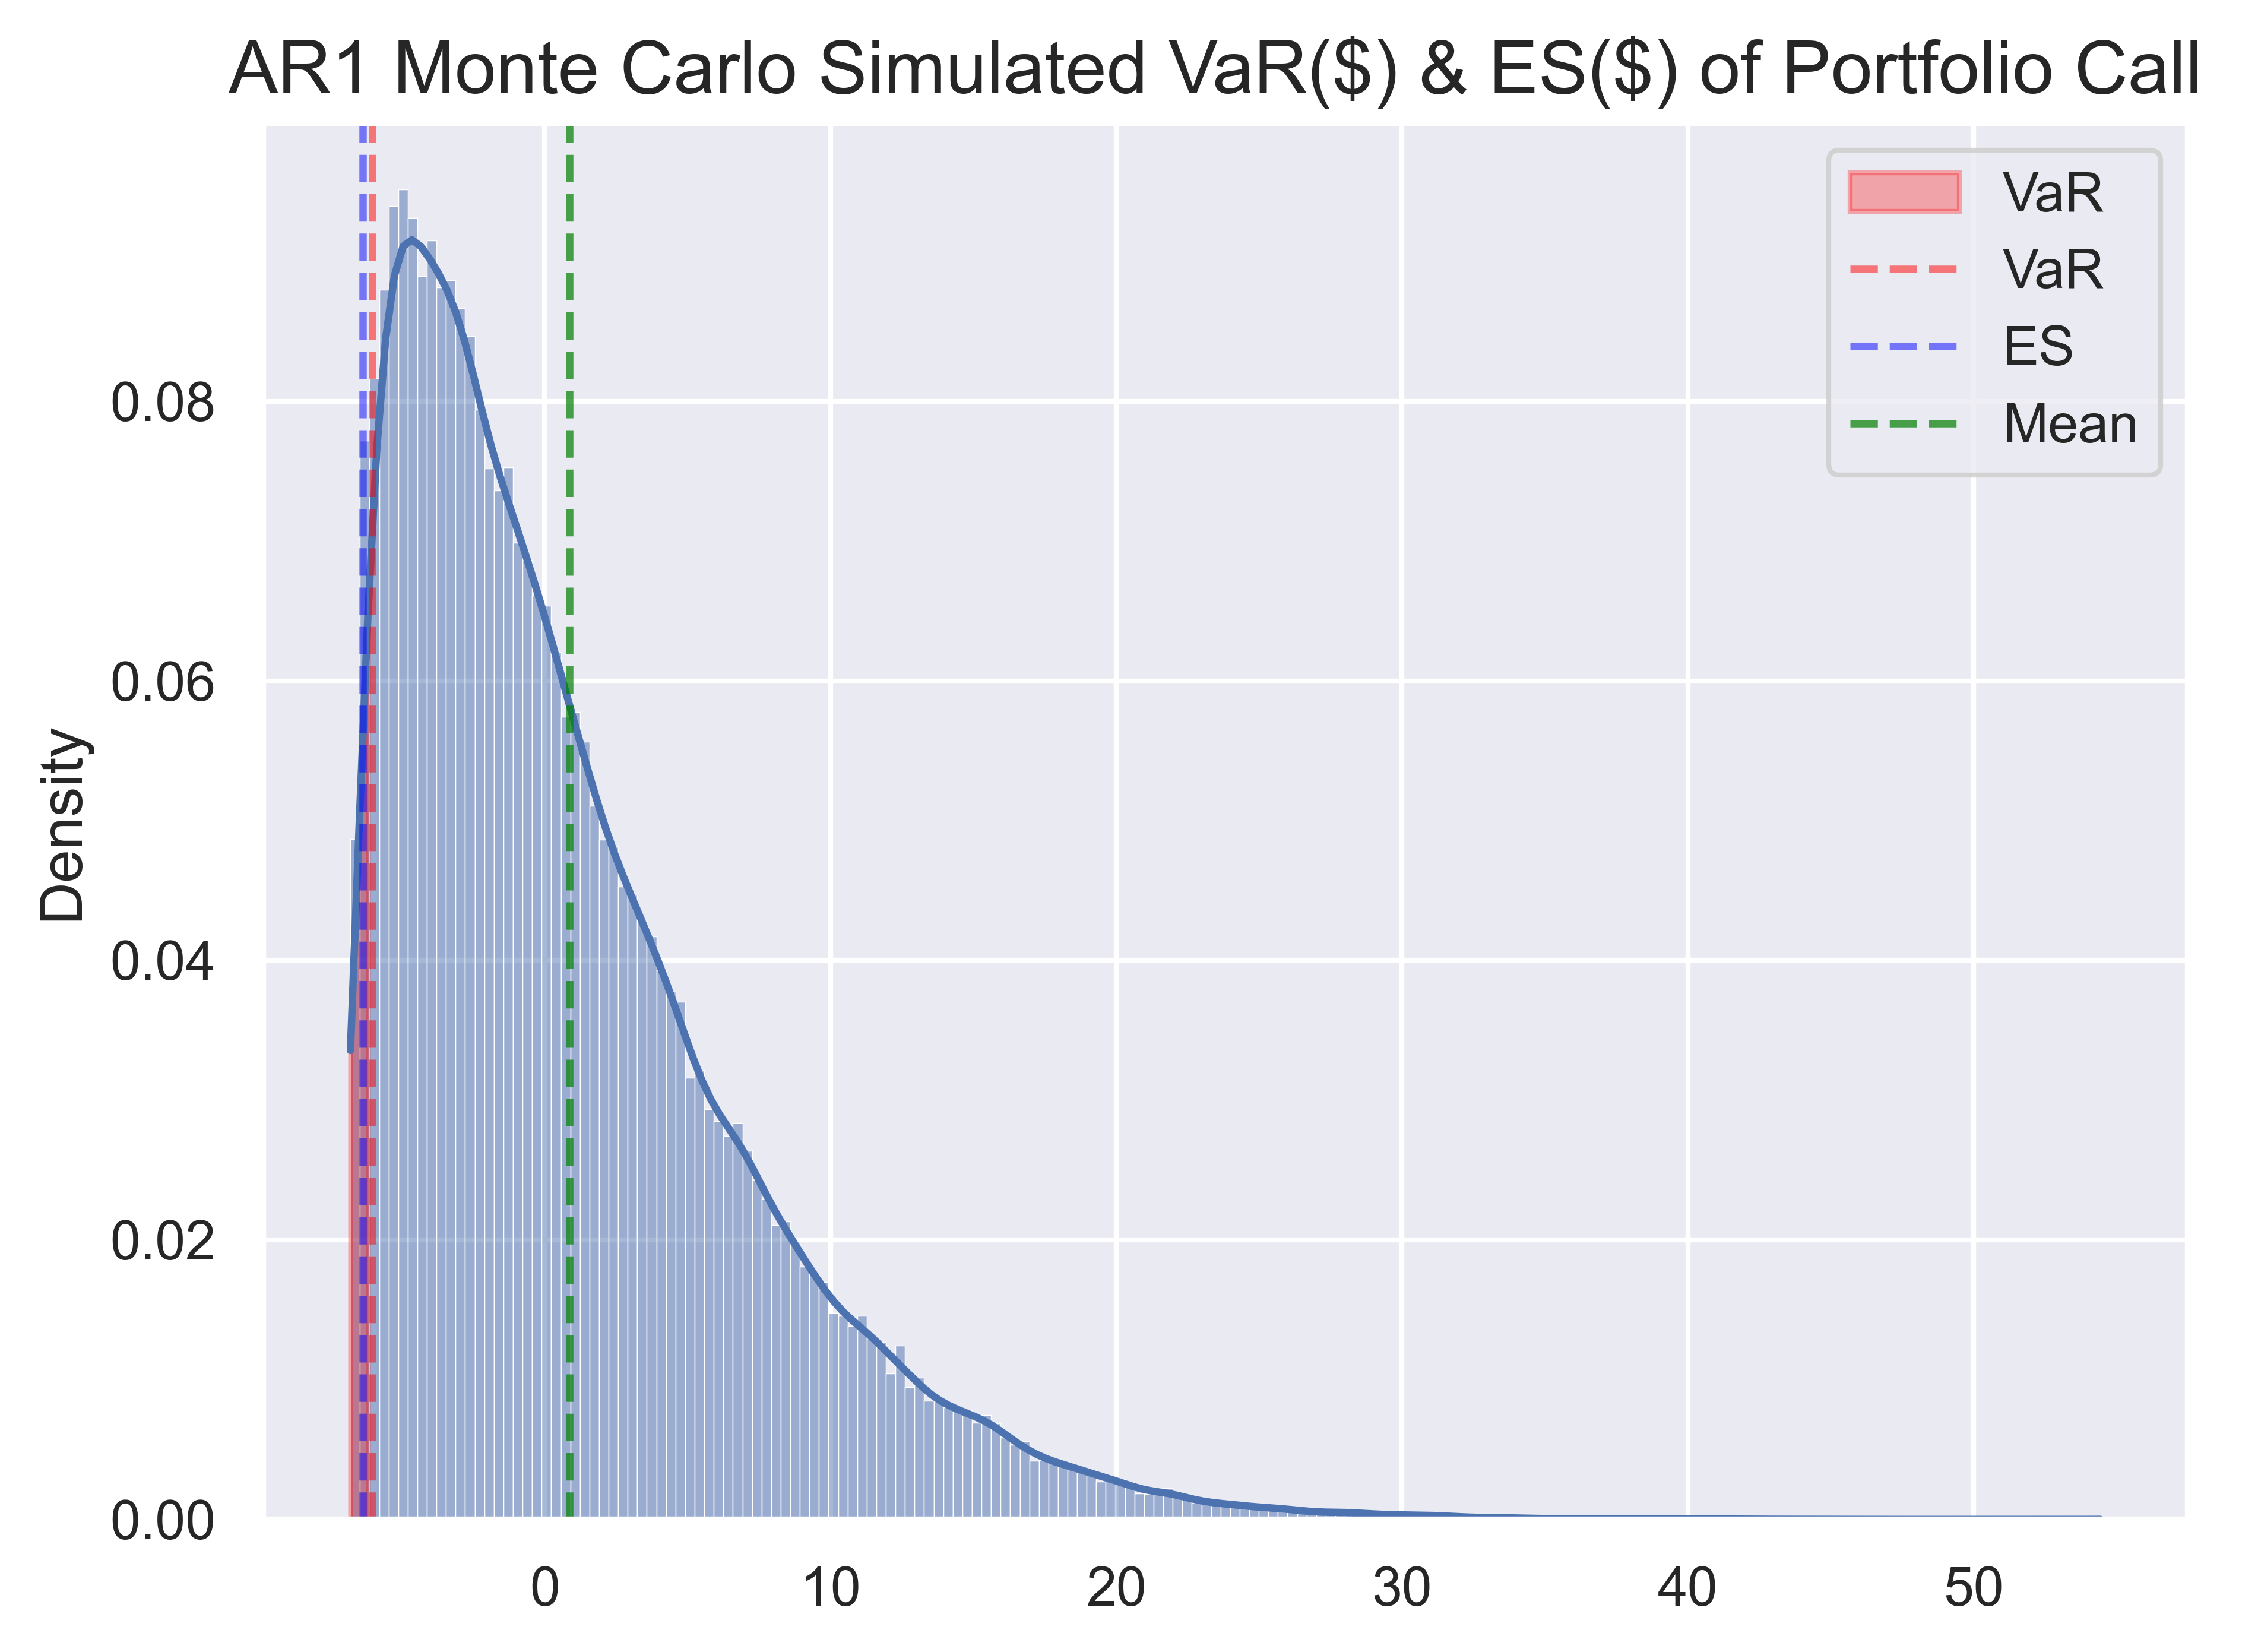
\includegraphics[width=0.45\textwidth]{./image/image_3/Simulation/Call.png} 
    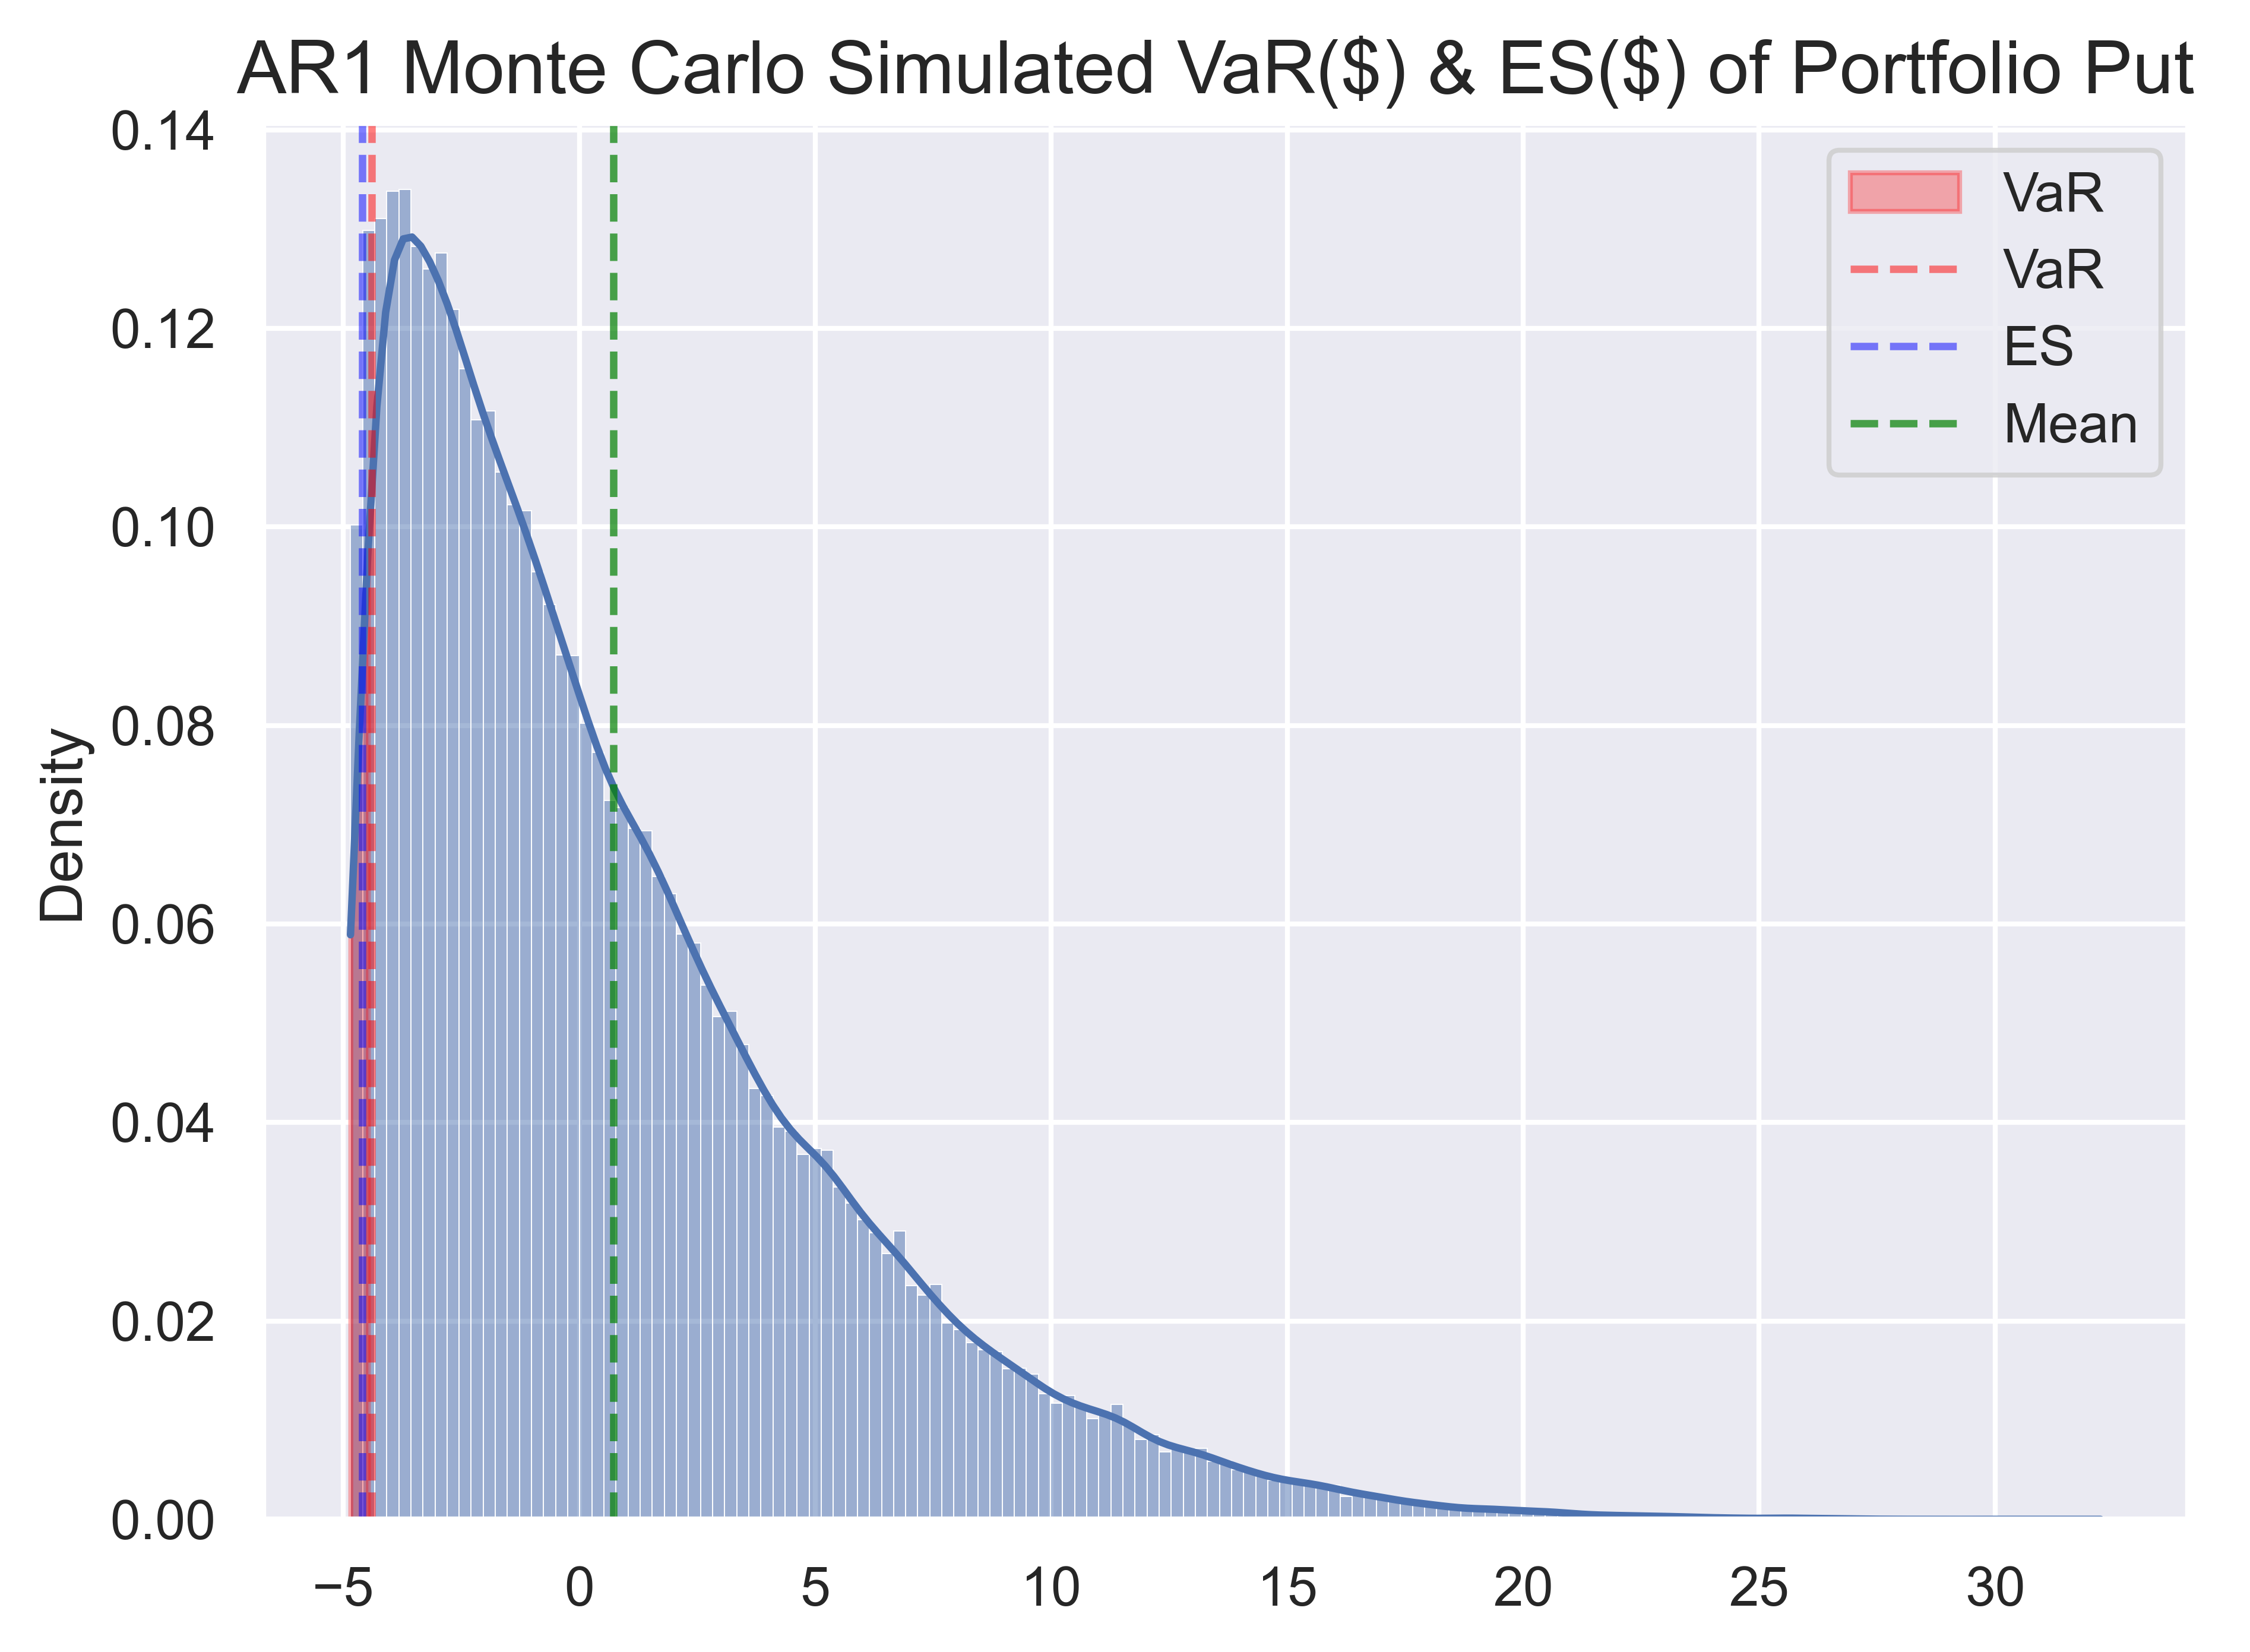
\includegraphics[width=0.45\textwidth]{./image/image_3/Simulation/Put.png} 
    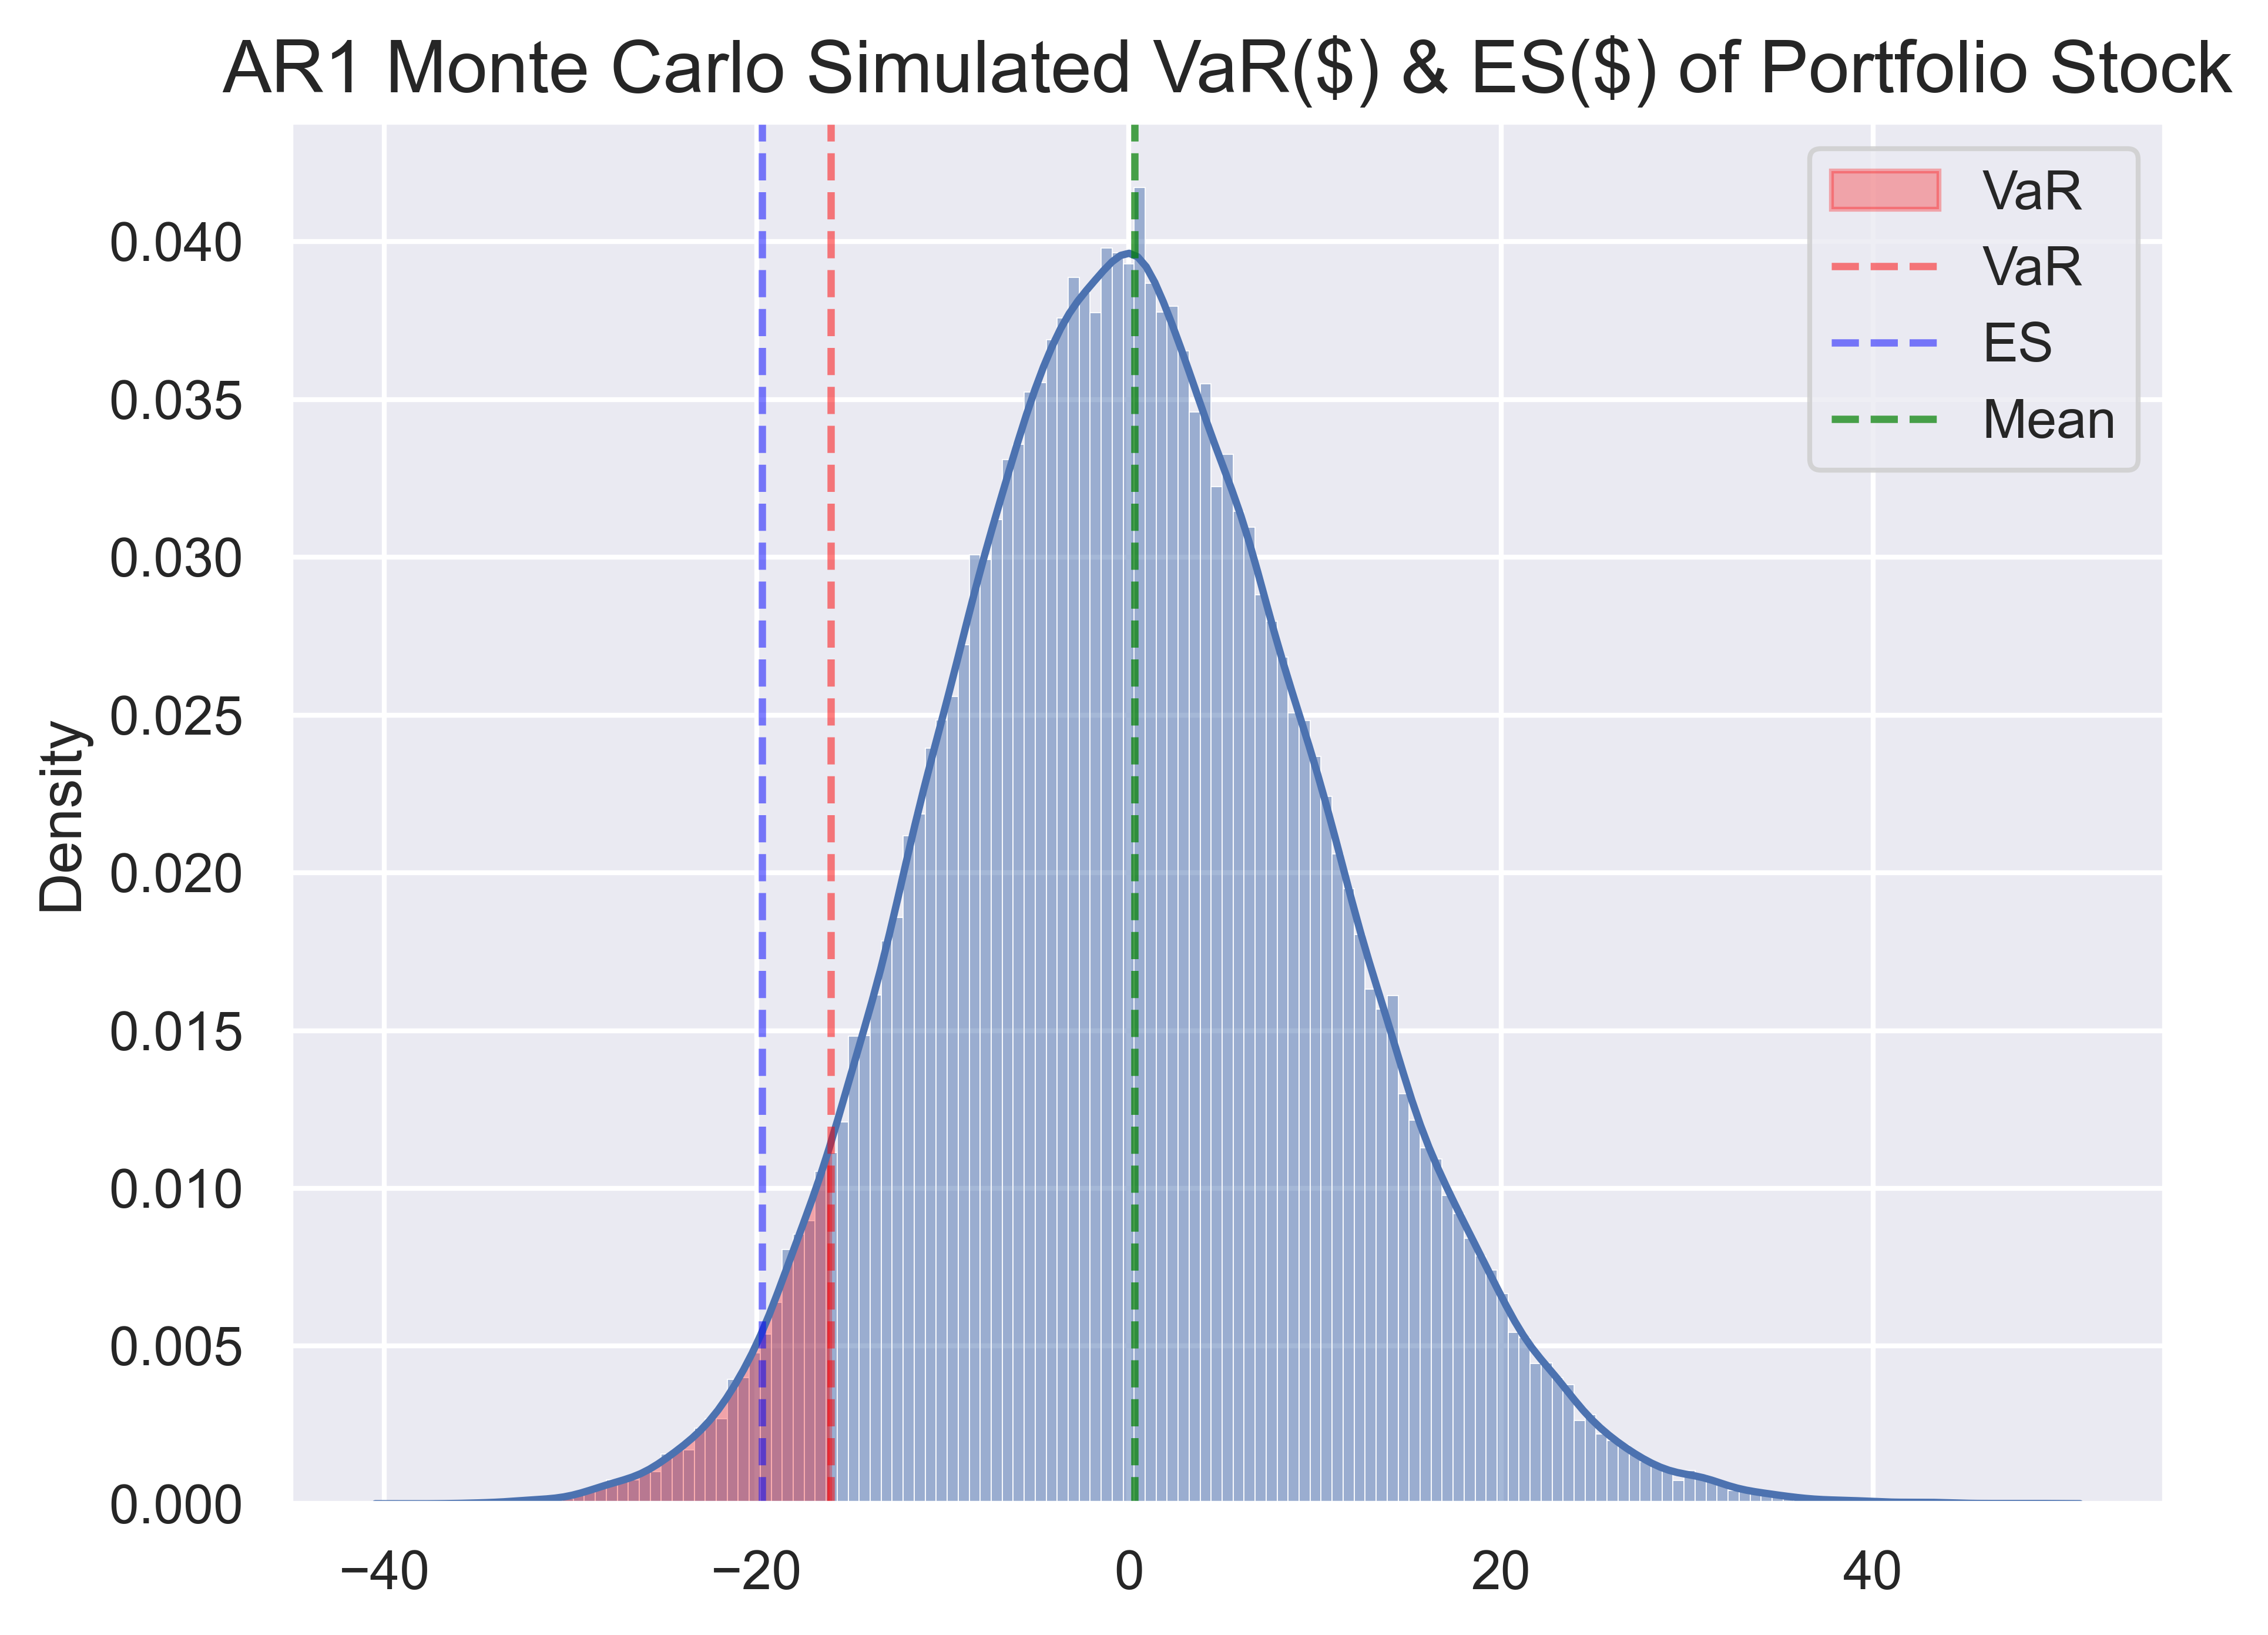
\includegraphics[width=0.45\textwidth]{./image/image_3/Simulation/Stock.png}
    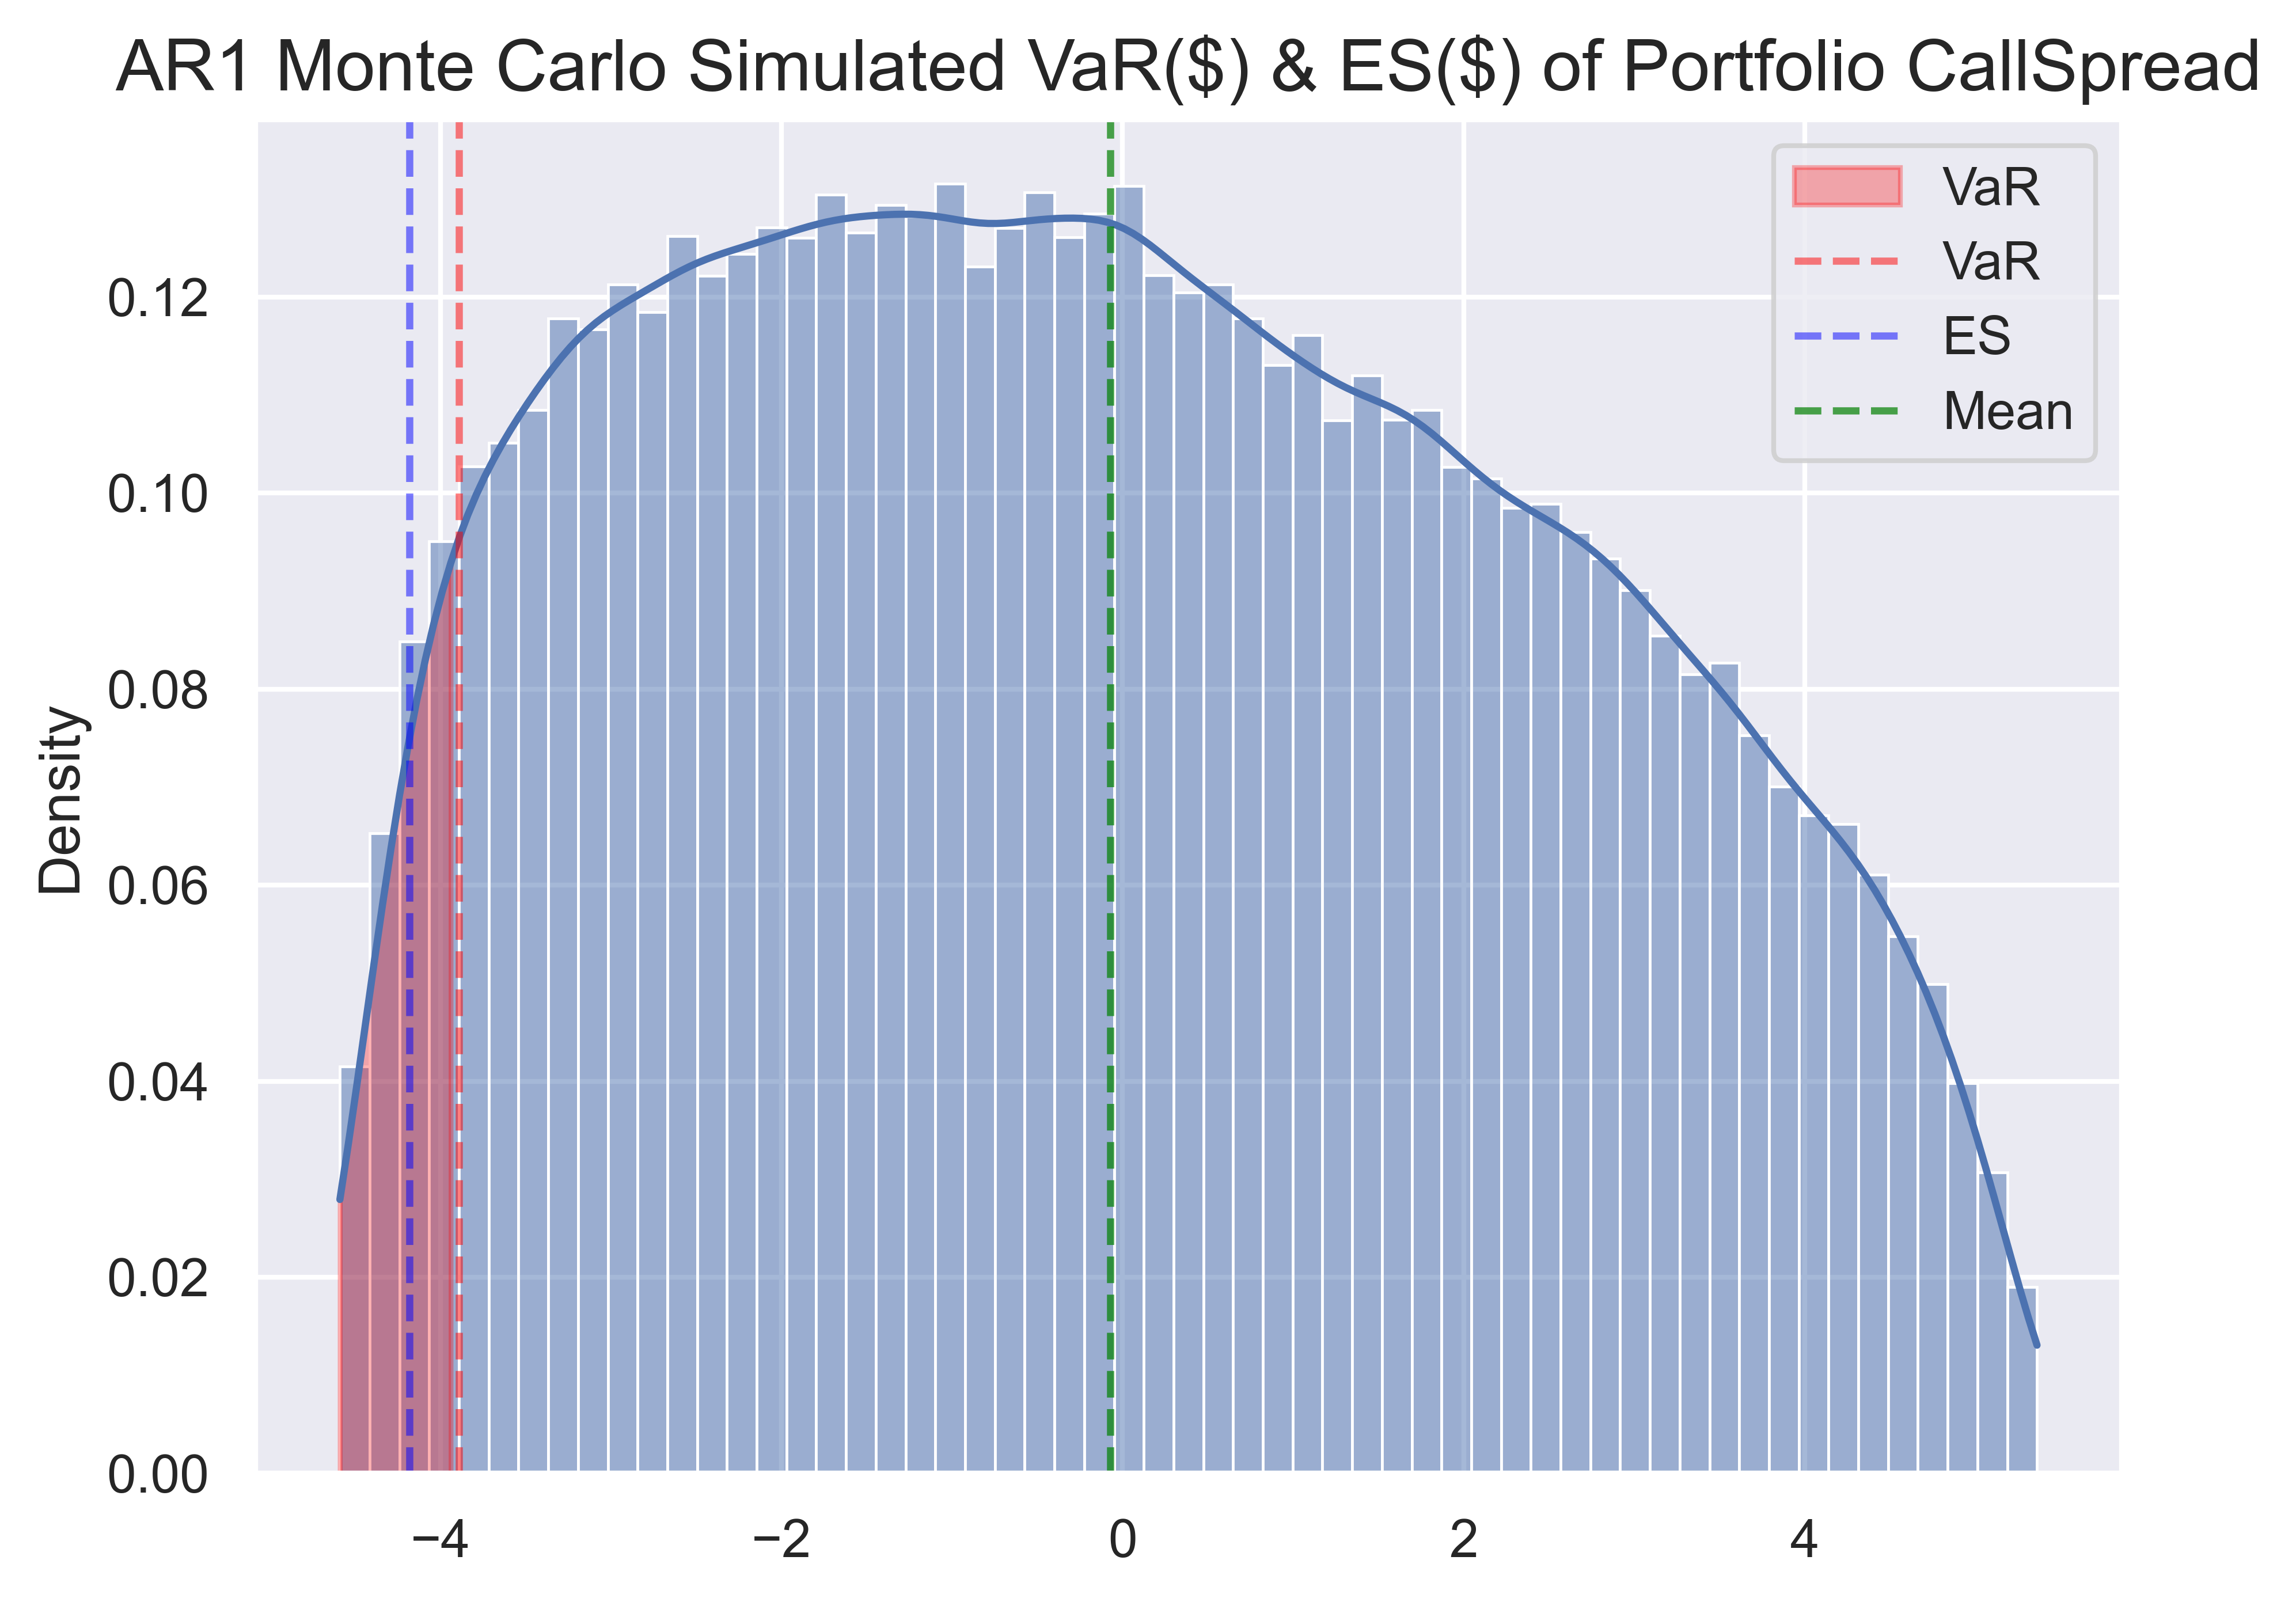
\includegraphics[width=0.45\textwidth]{./image/image_3/Simulation/CallSpread.png} 
    \caption{Simulated Portfolio Value 10 Days Later}
\end{figure}

\begin{figure}[htbp] 
    \centering 
    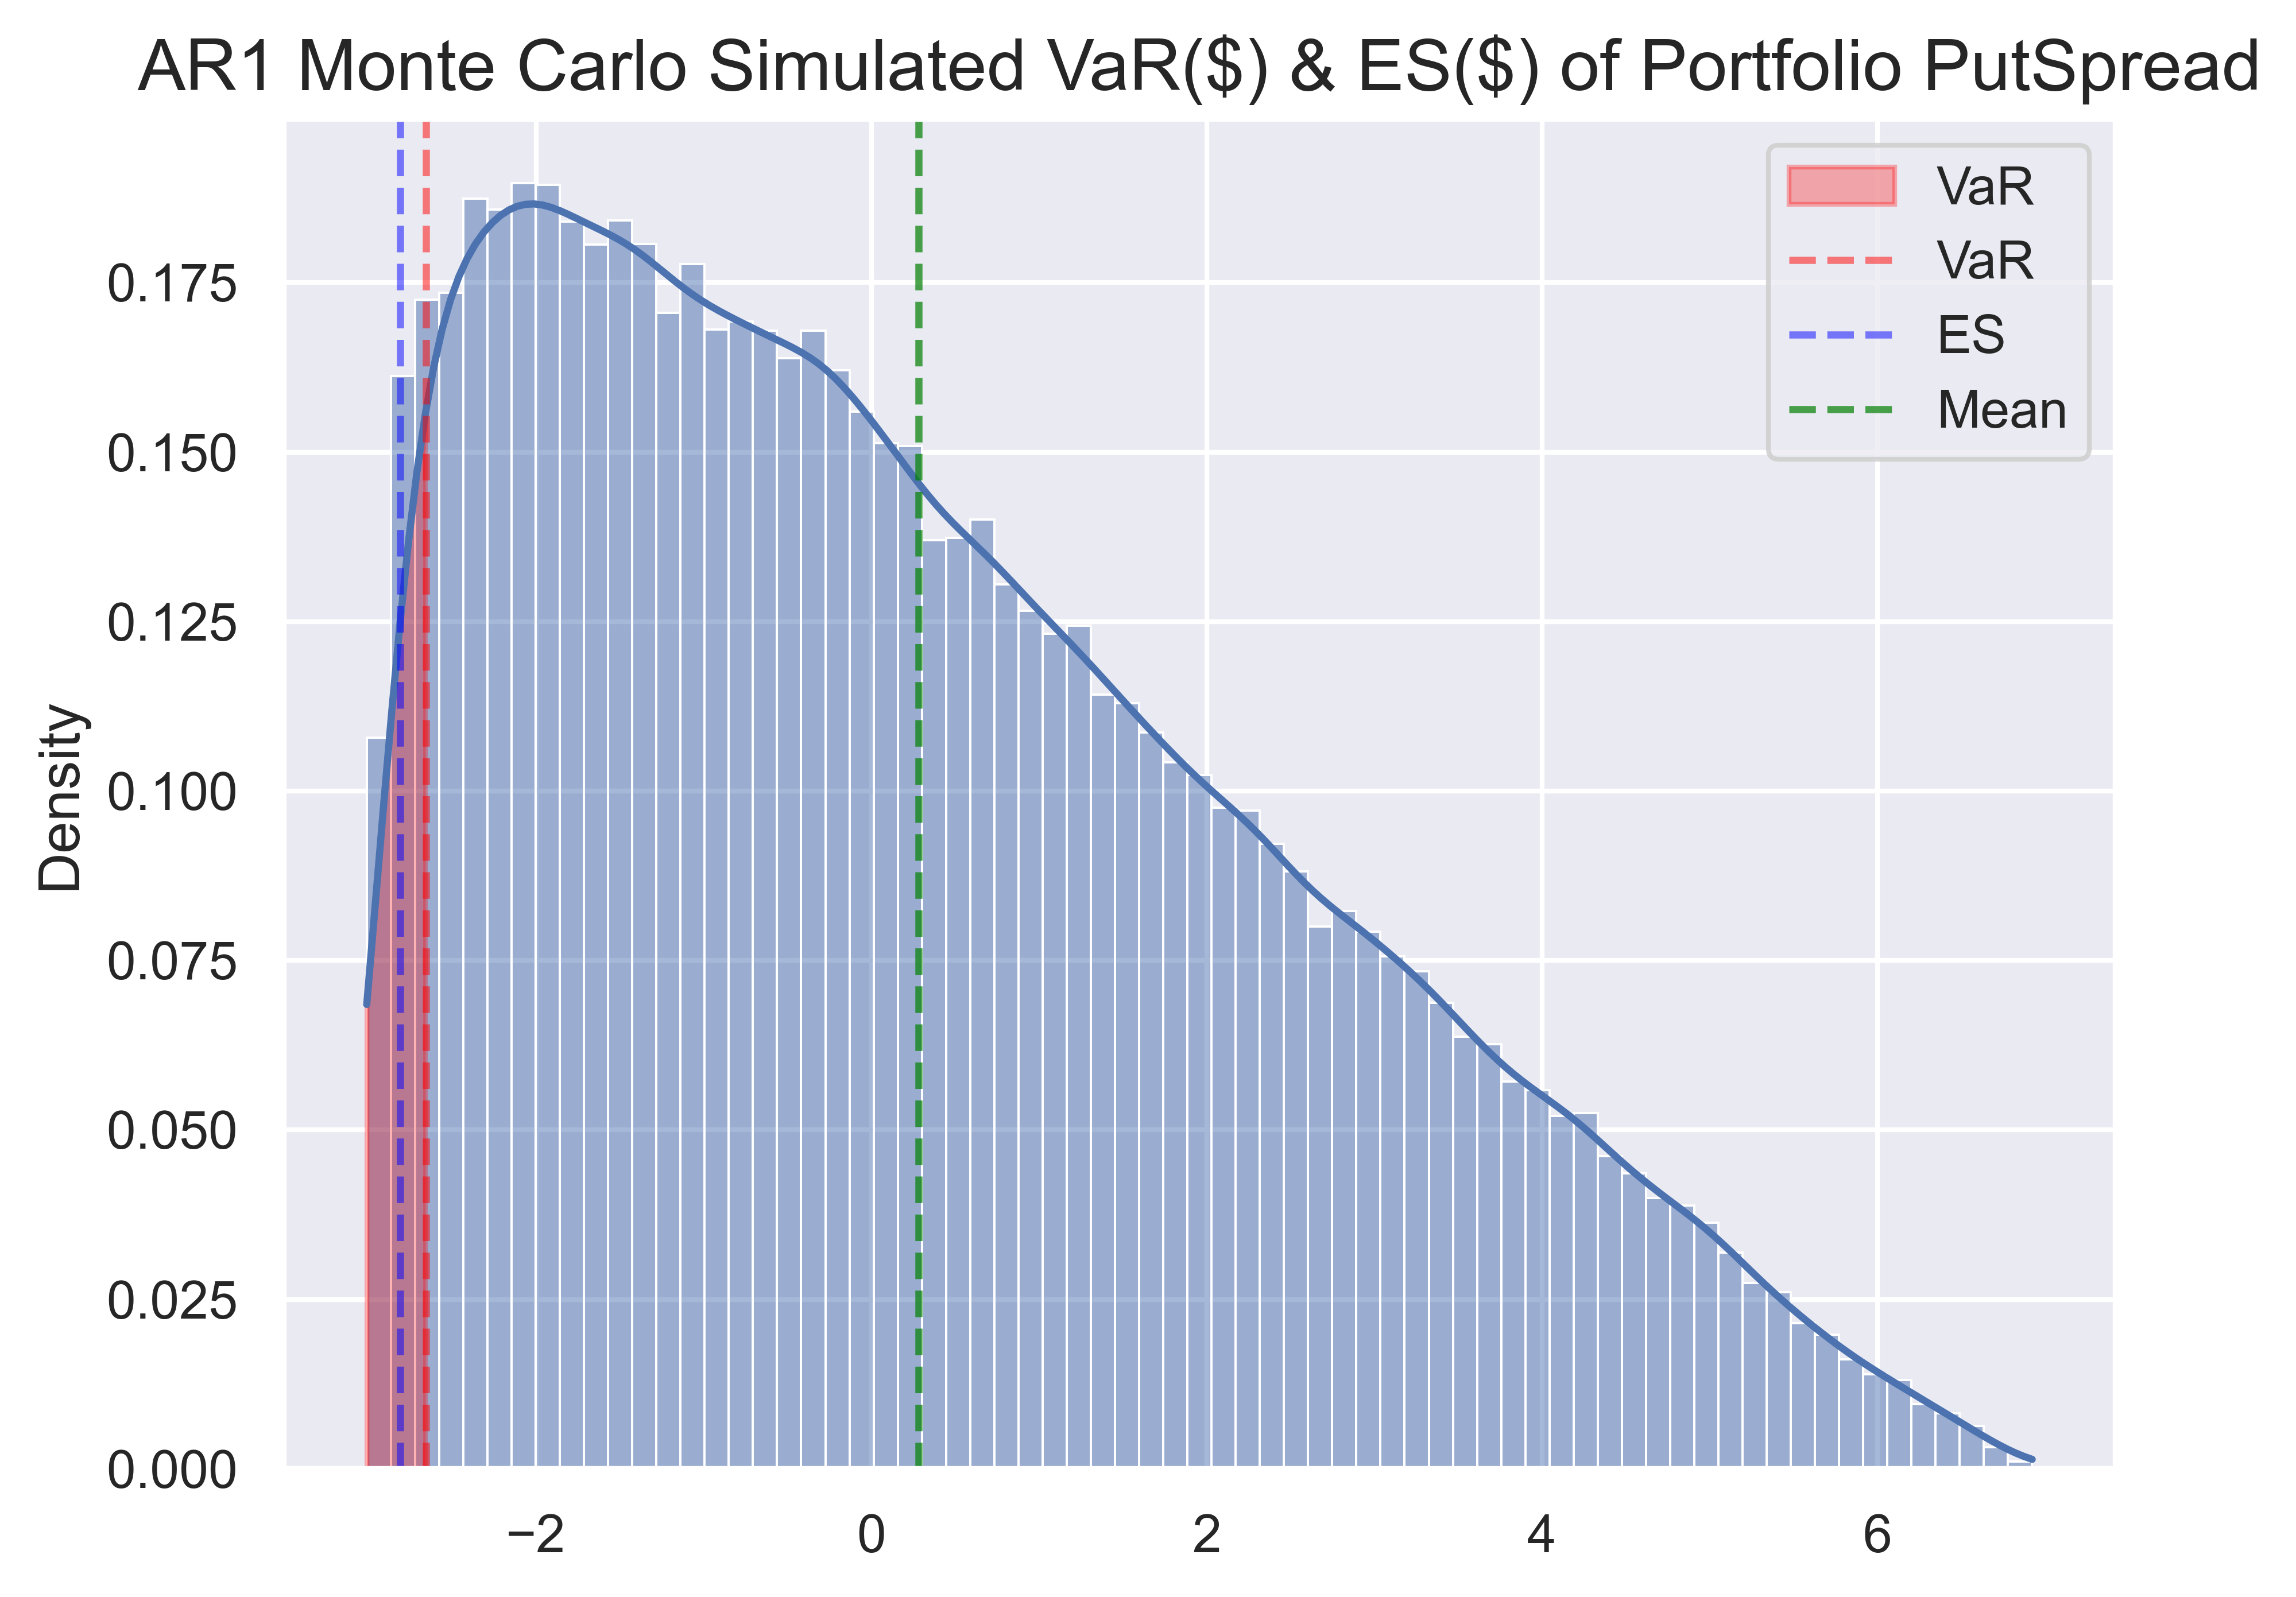
\includegraphics[width=0.45\textwidth]{./image/image_3/Simulation/PutSpread.png} 
    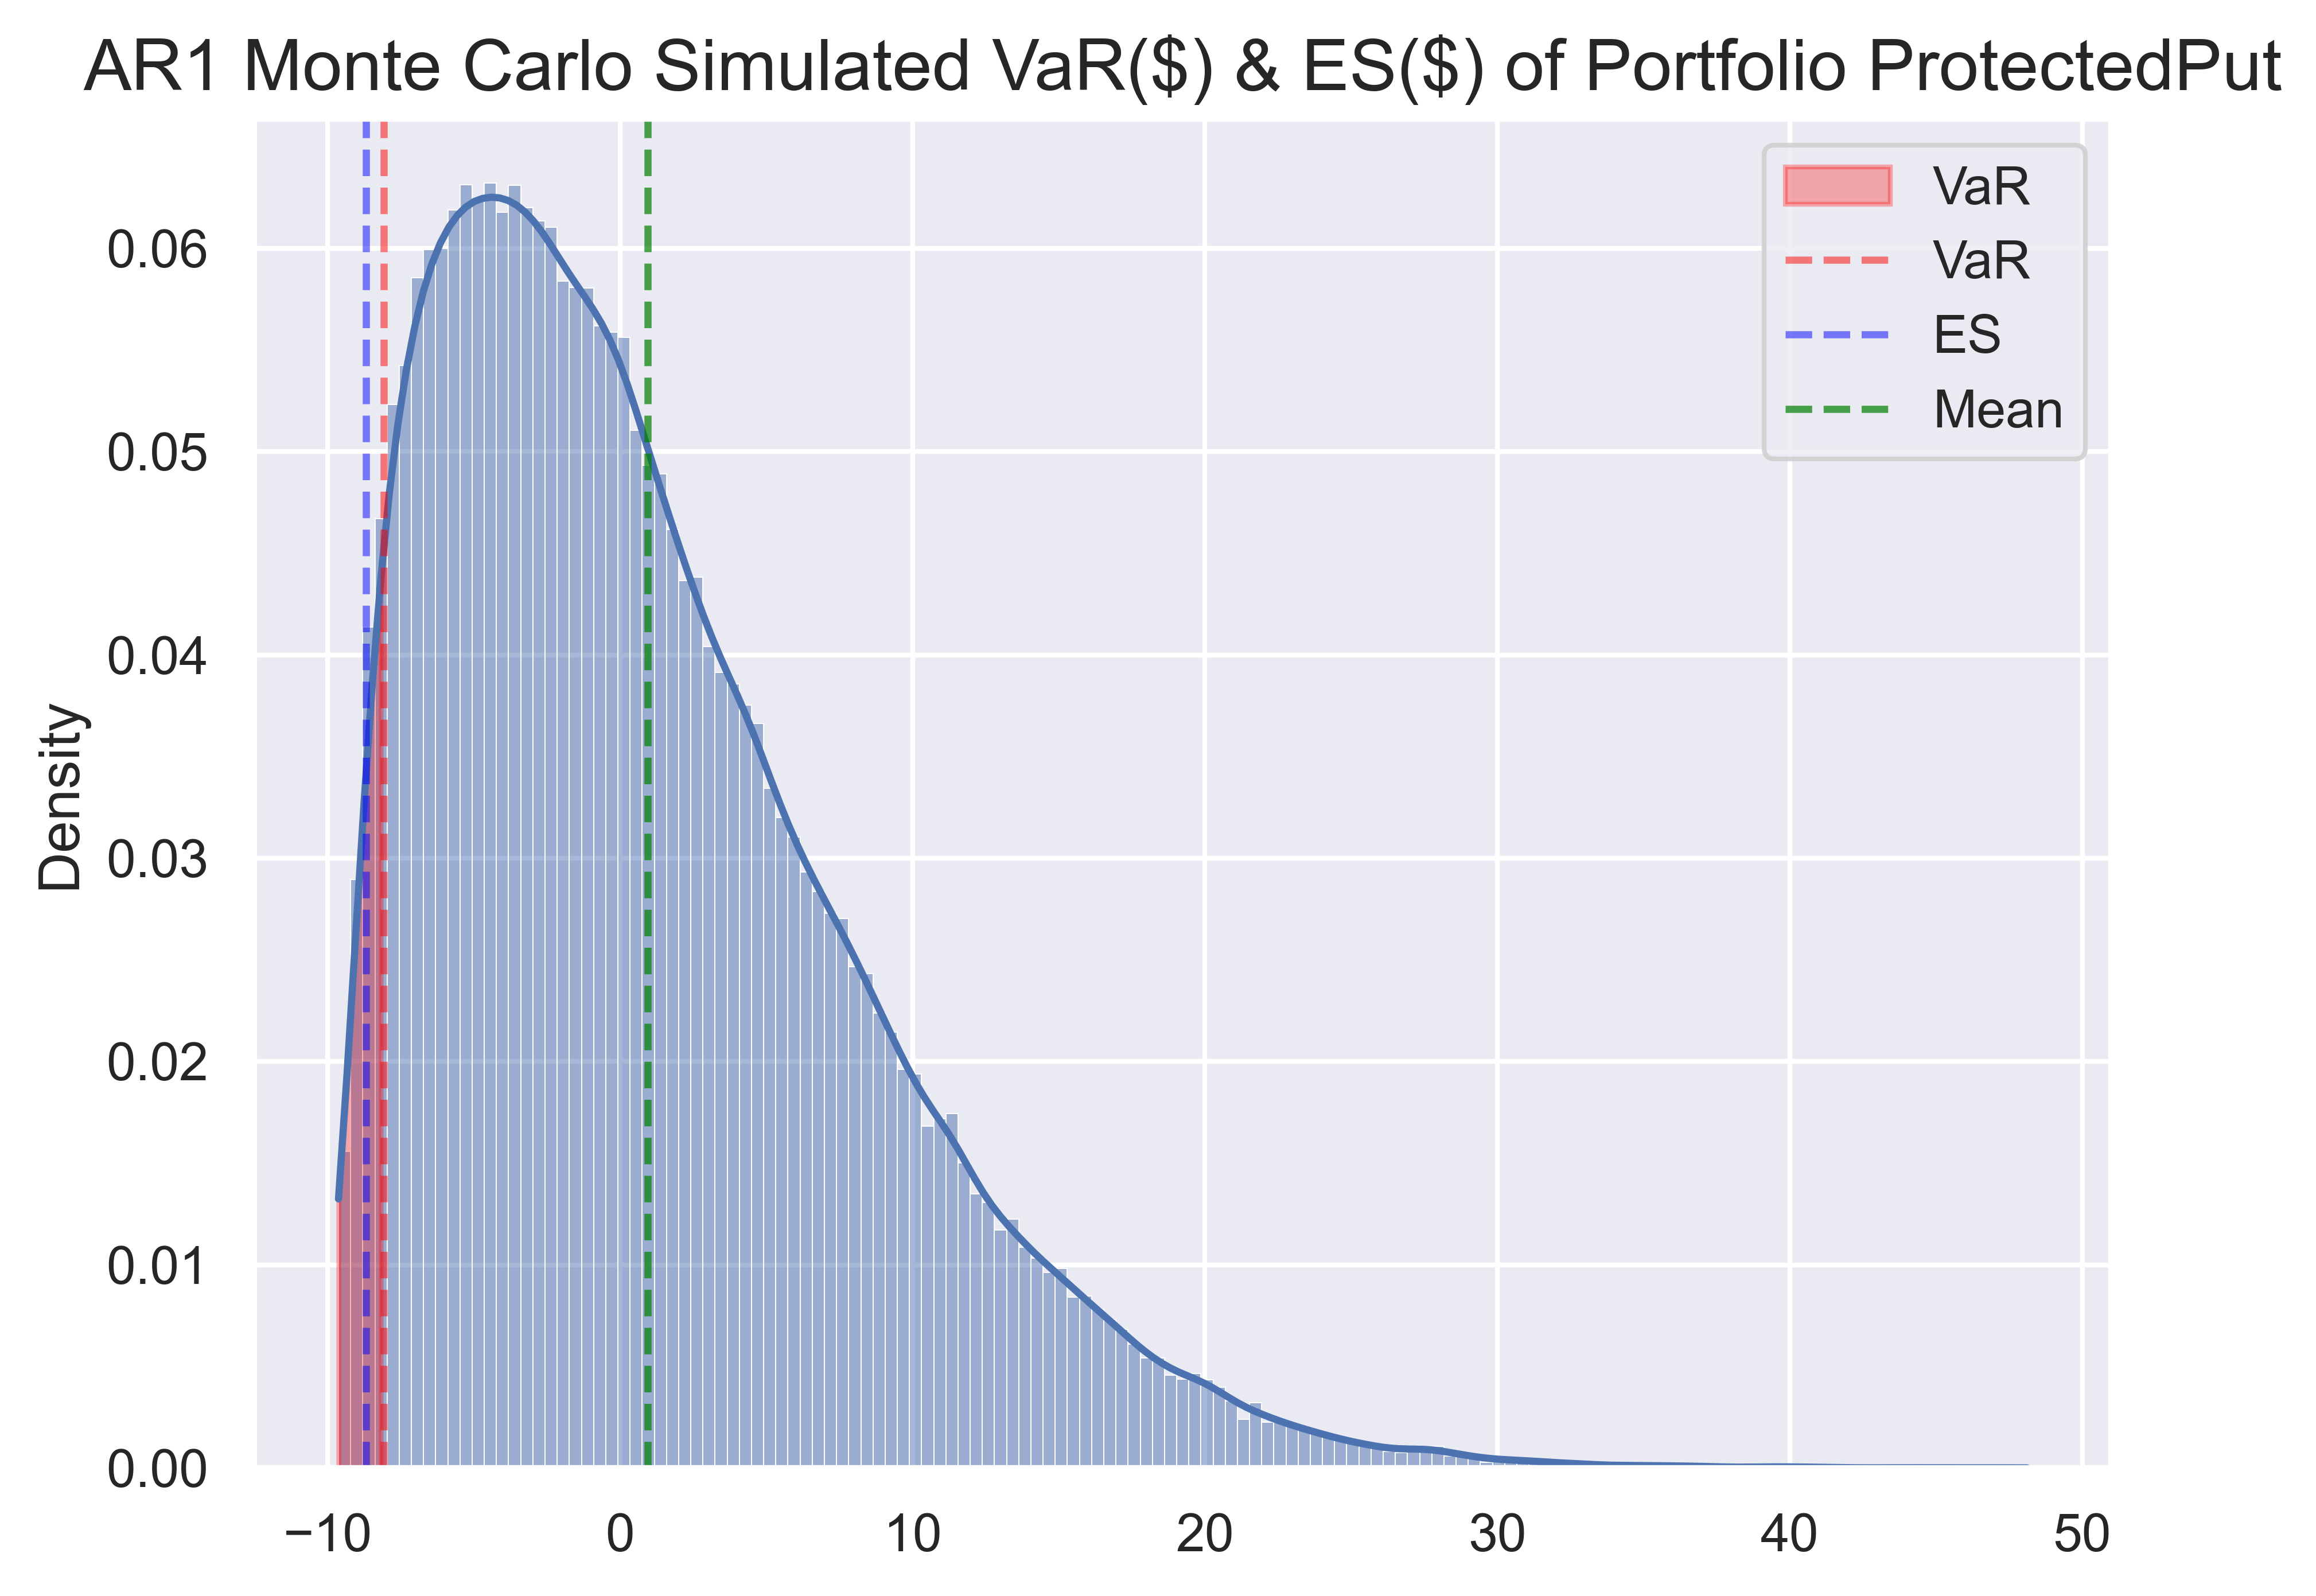
\includegraphics[width=0.45\textwidth]{./image/image_3/Simulation/ProtectedPut.png} 
    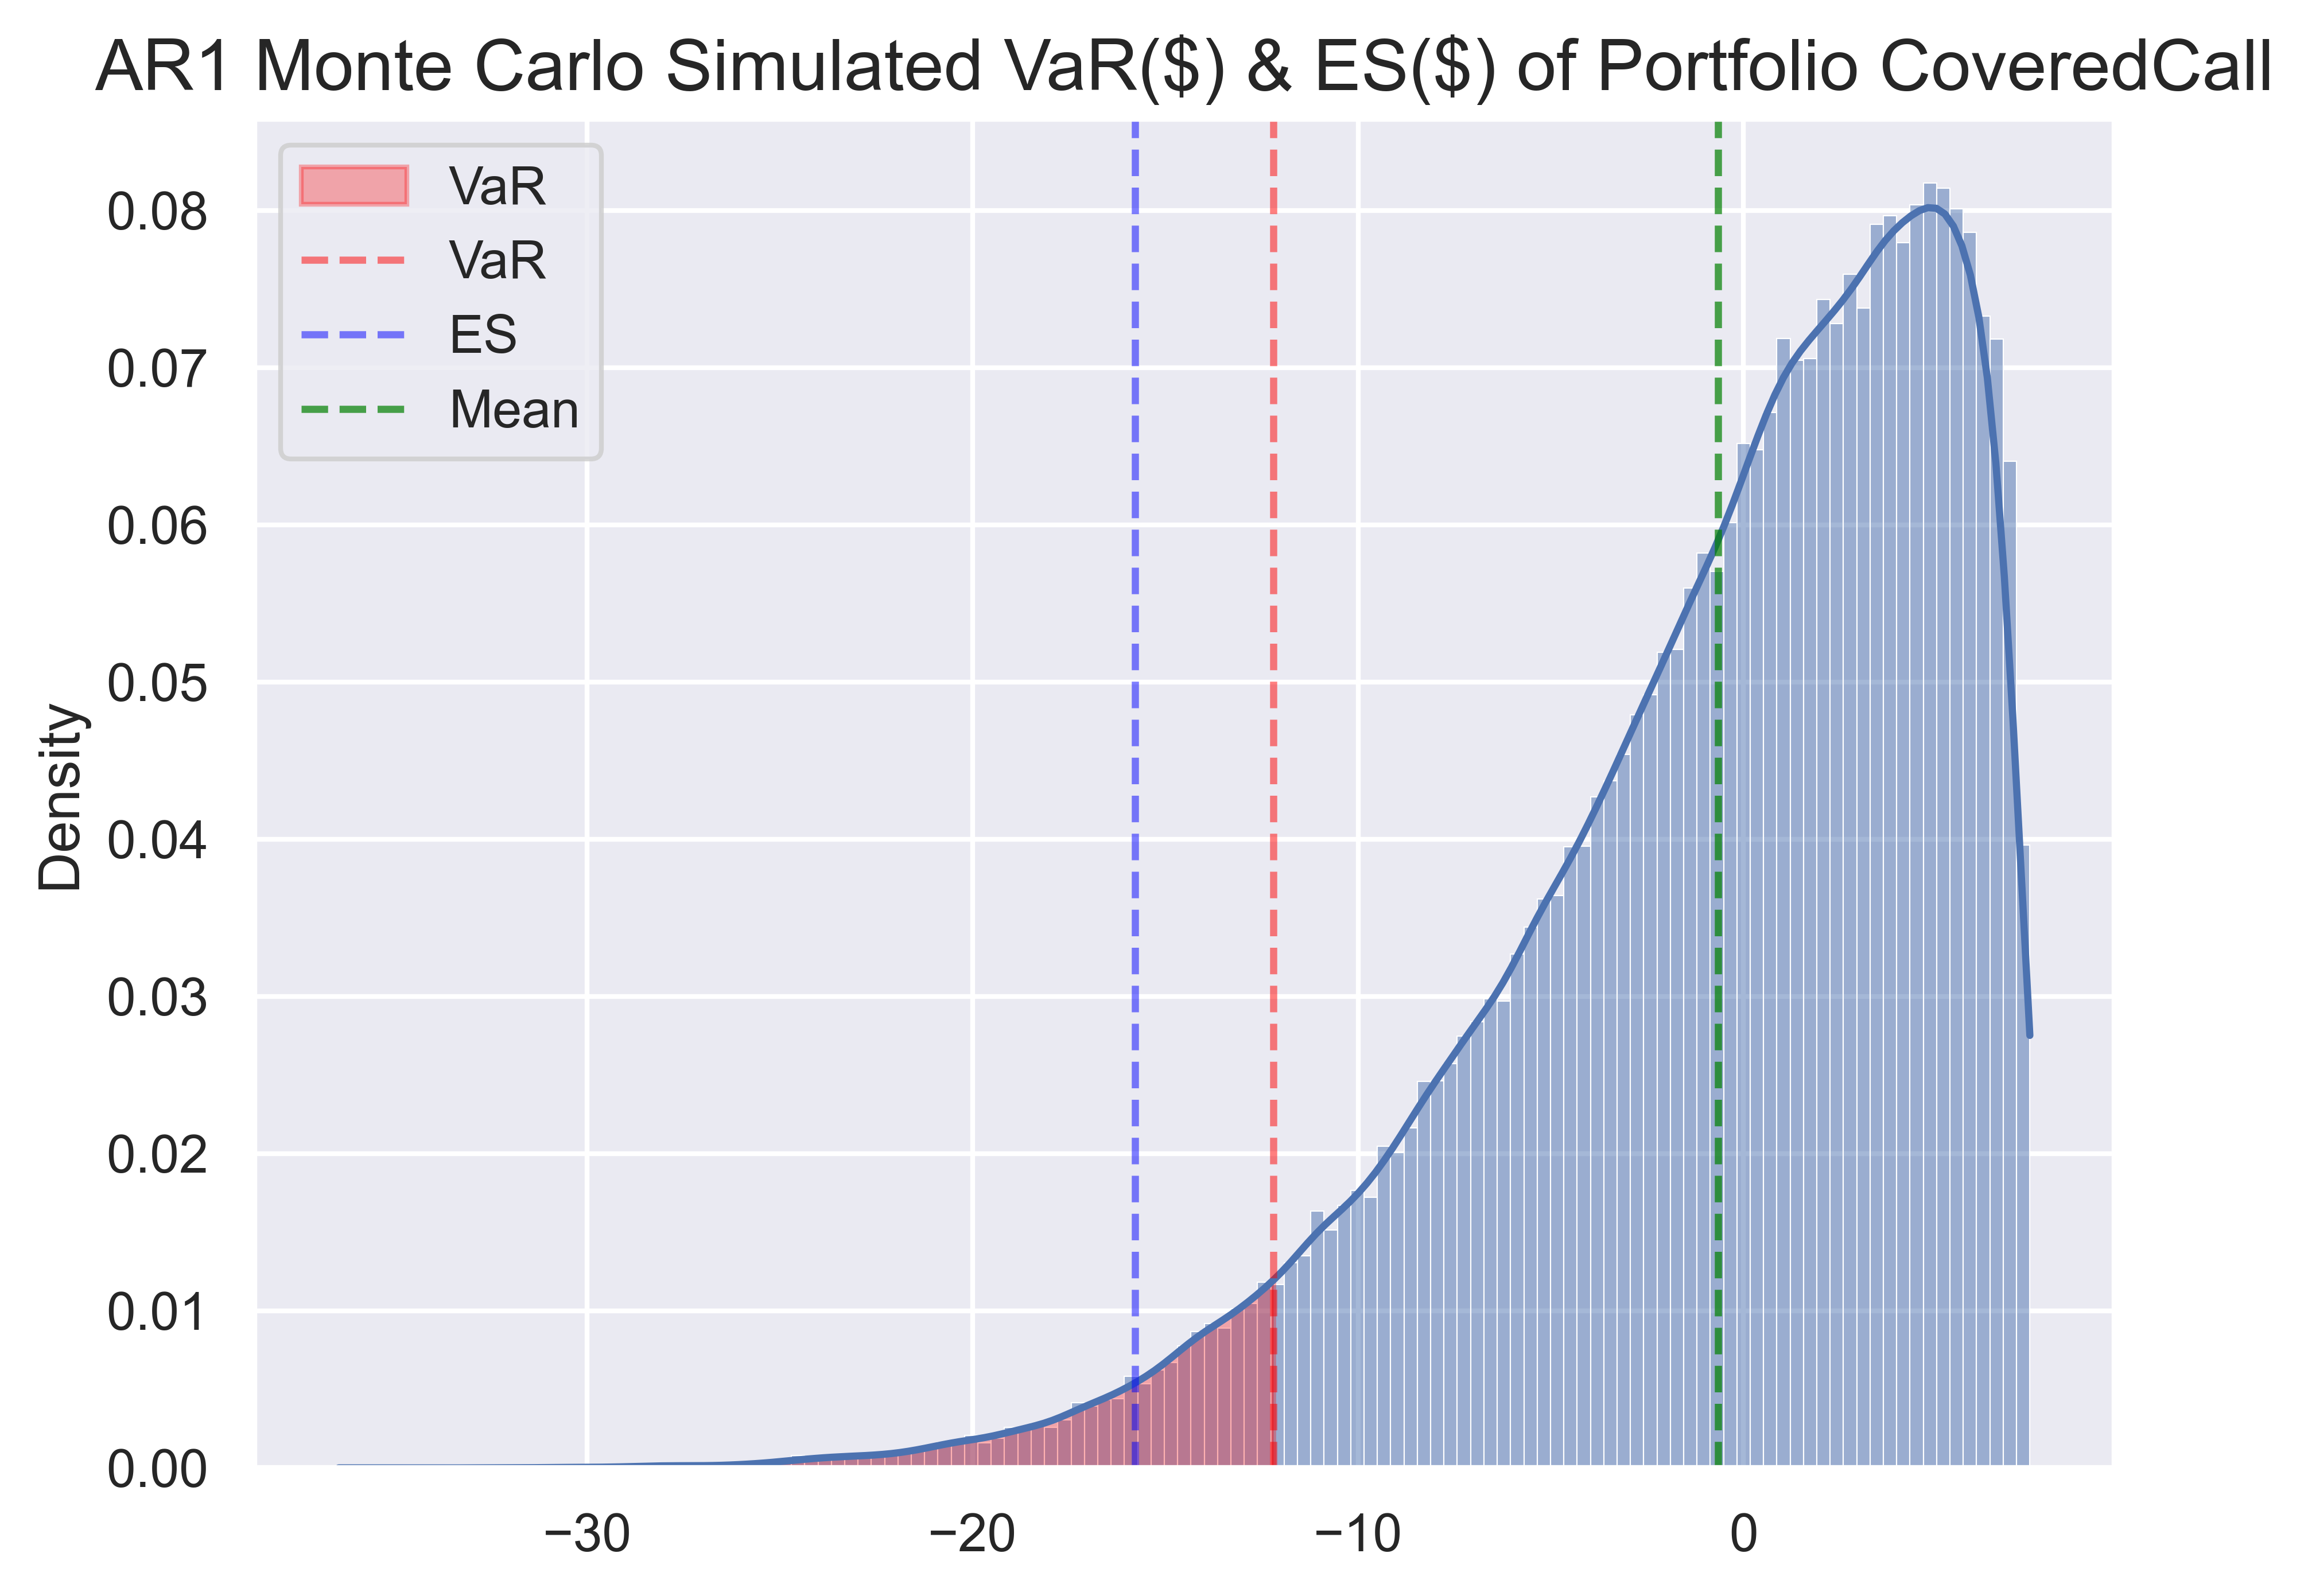
\includegraphics[width=0.45\textwidth]{./image/image_3/Simulation/CoveredCall.png} 
    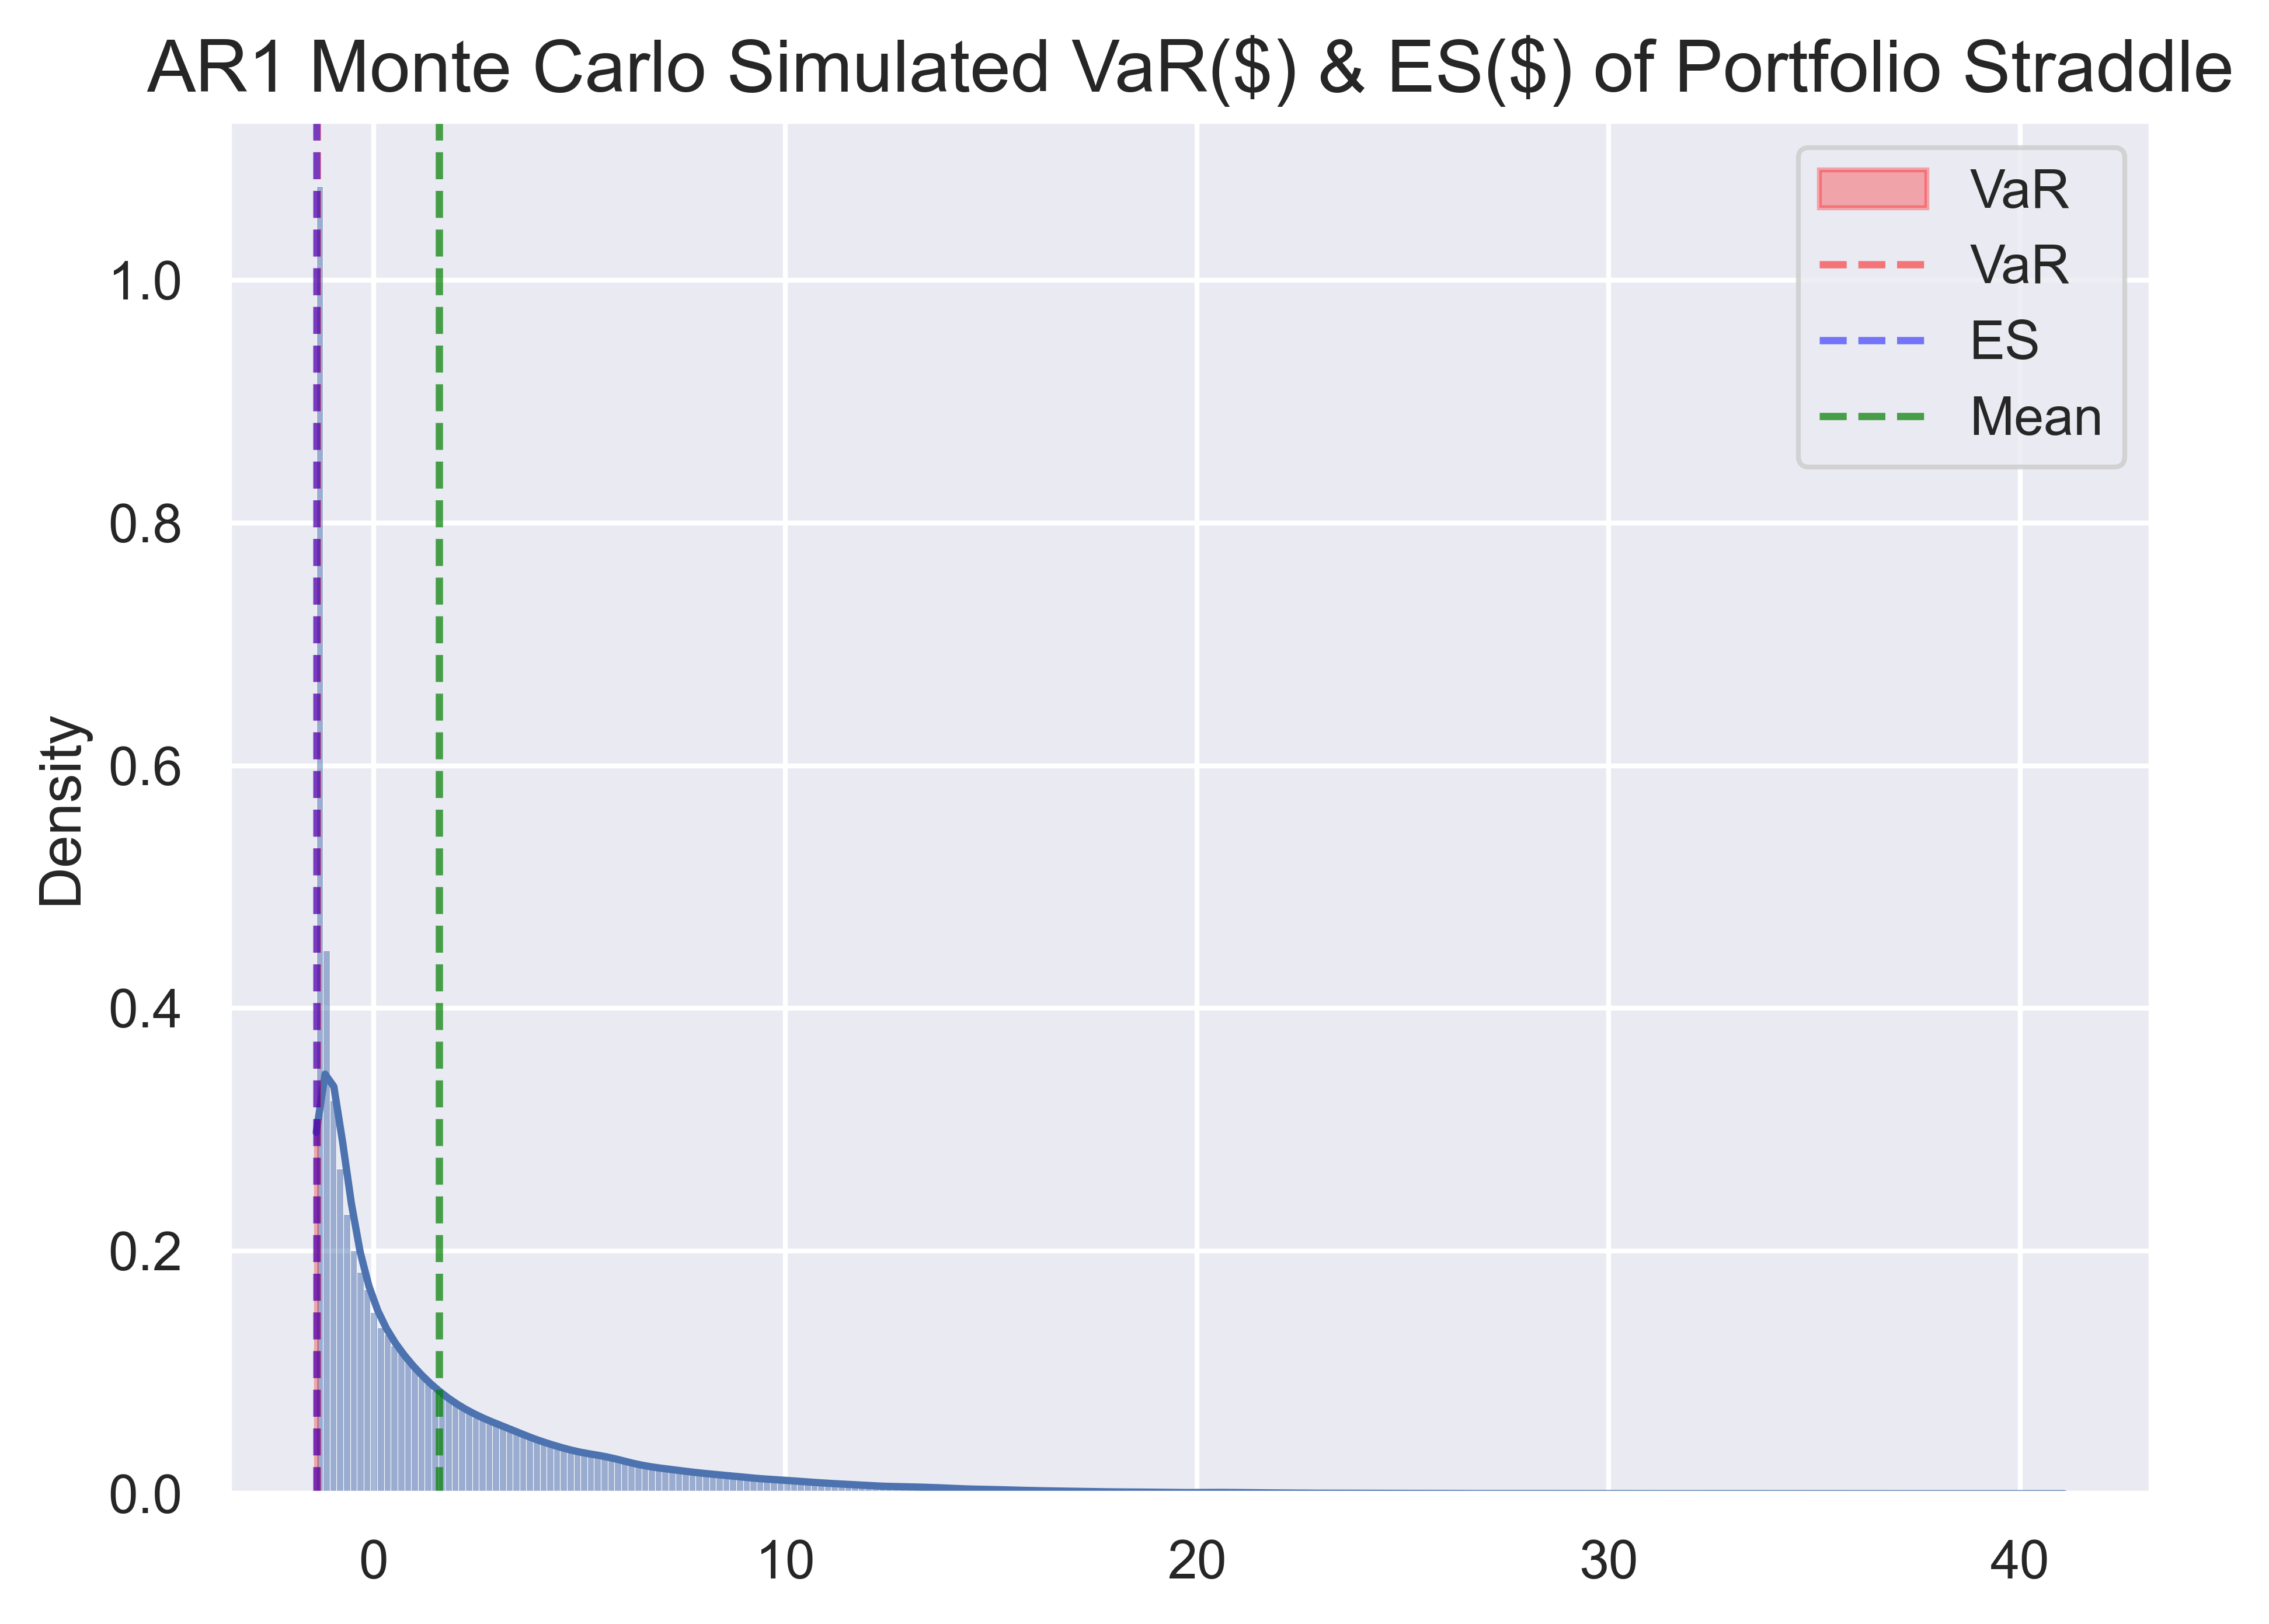
\includegraphics[width=0.45\textwidth]{./image/image_3/Simulation/Straddle.png} 
    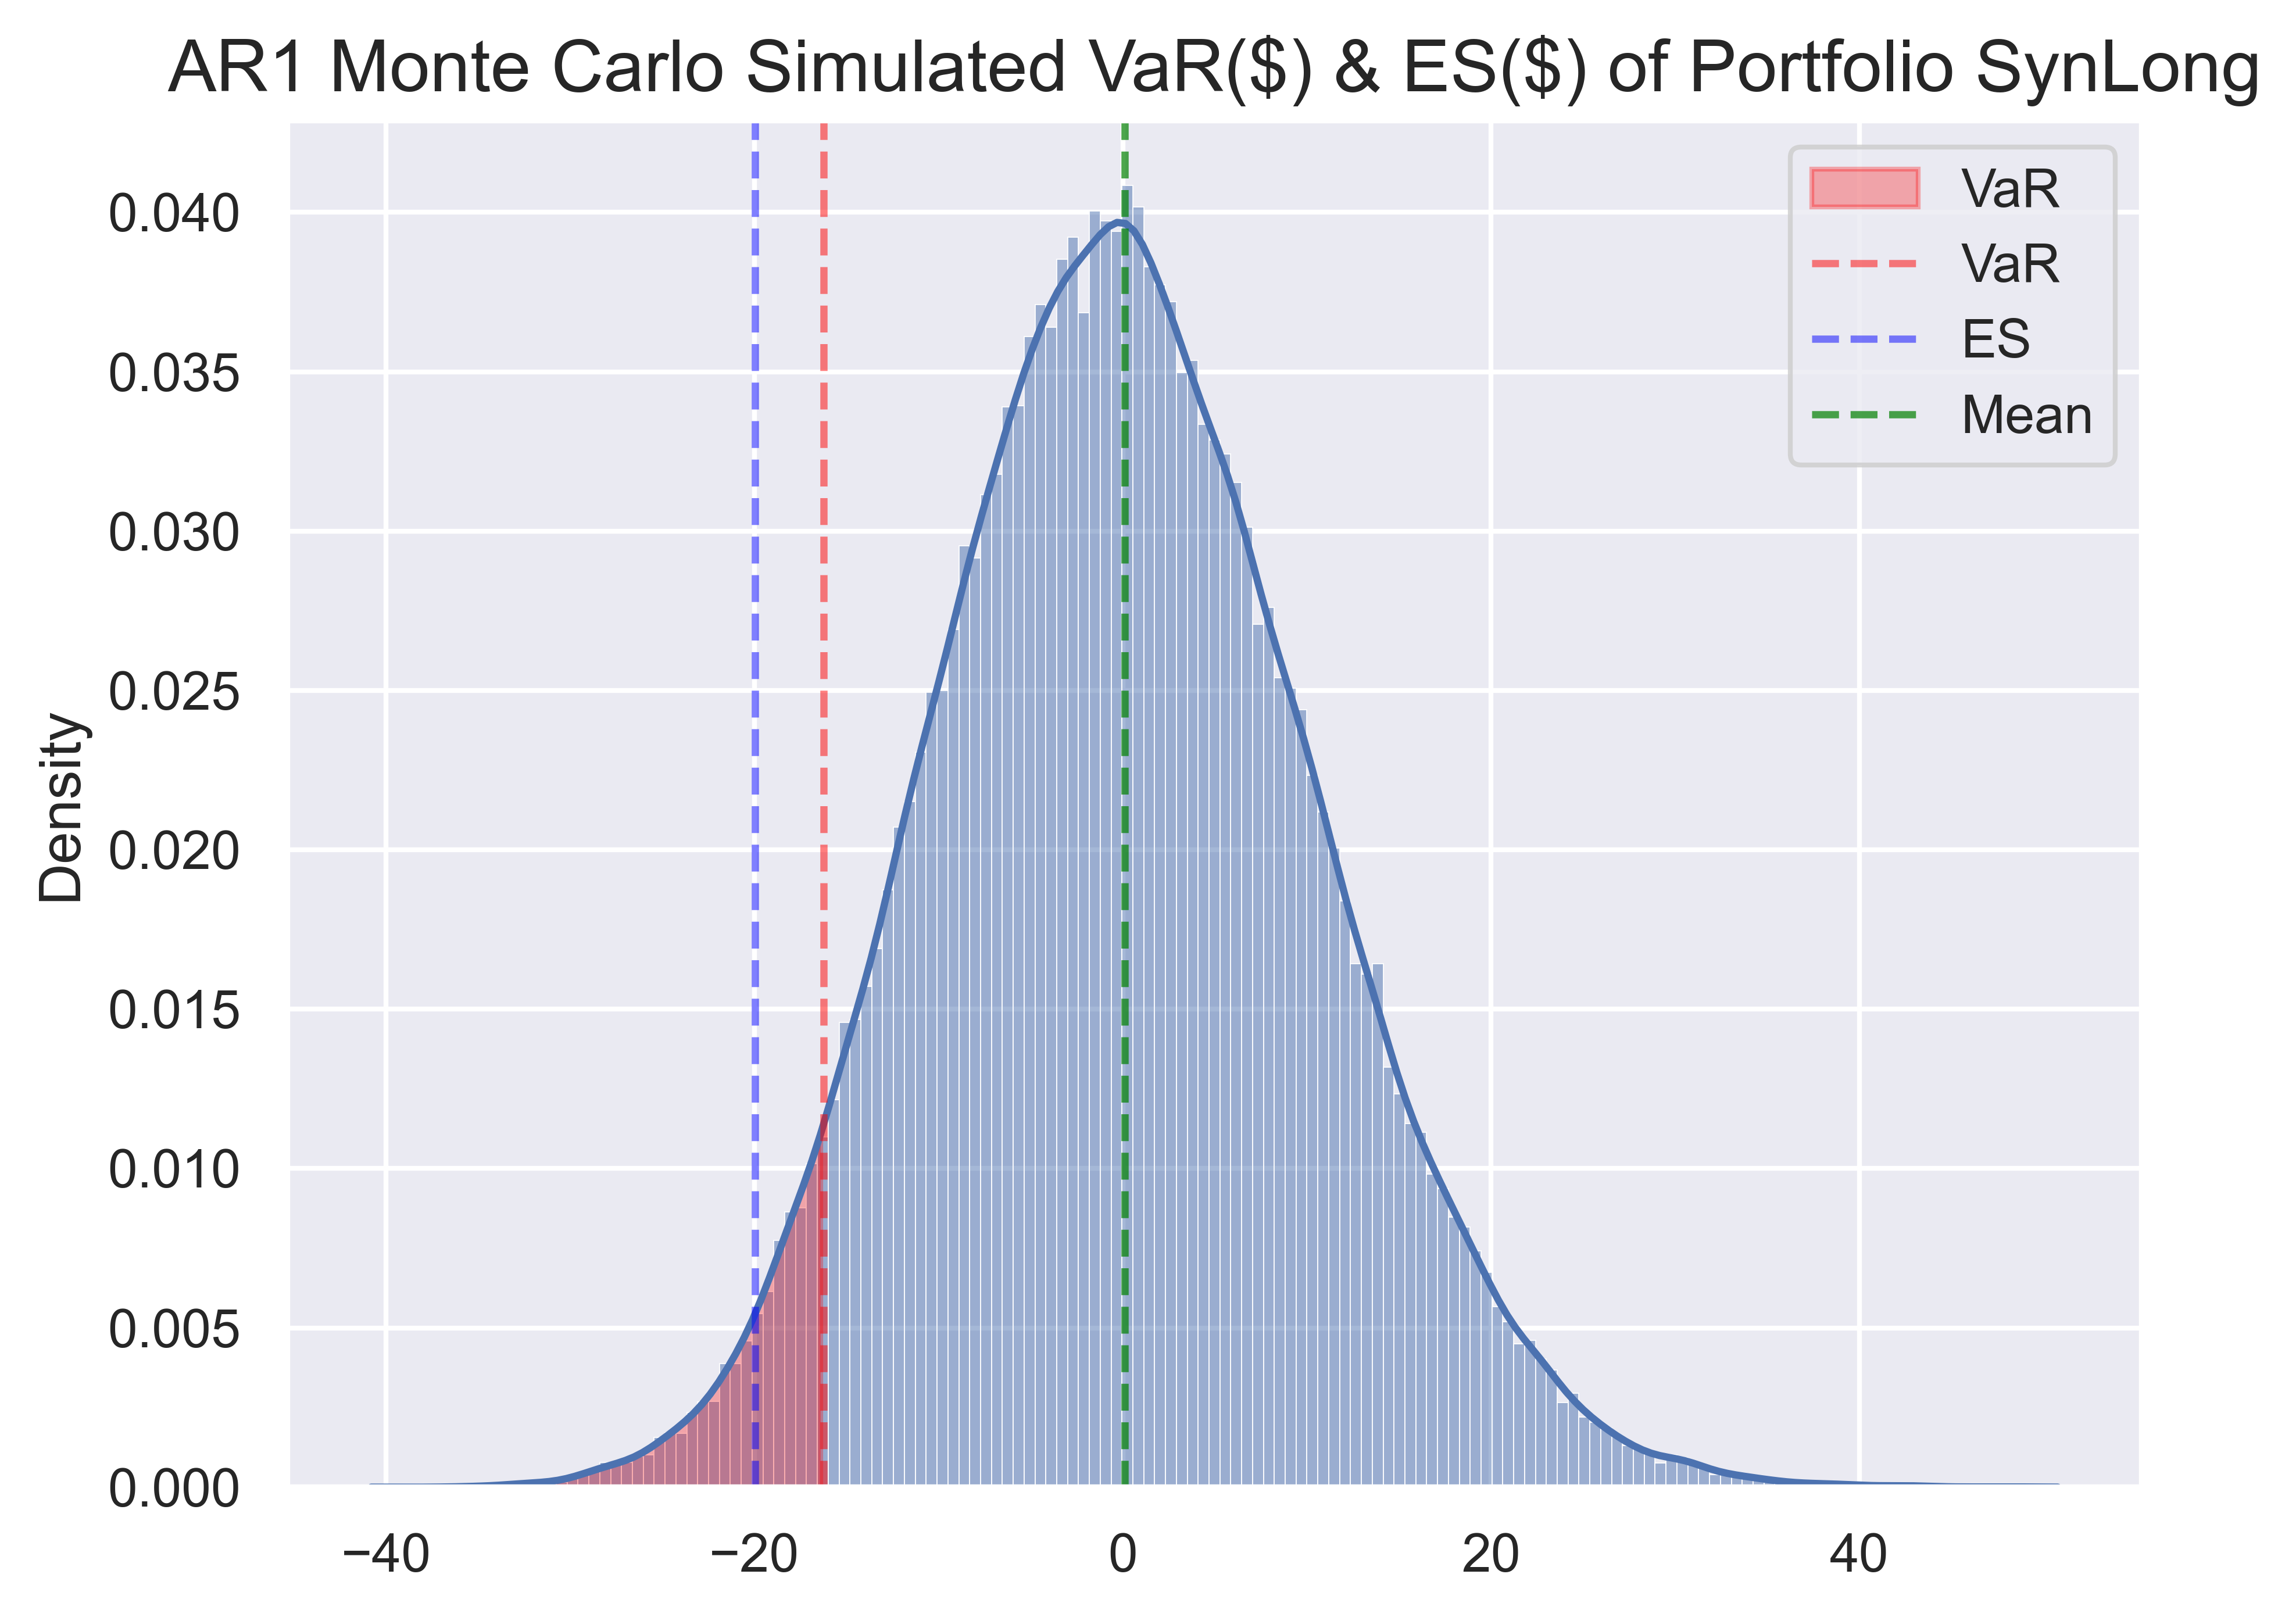
\includegraphics[width=0.45\textwidth]{./image/image_3/Simulation/SynLong.png} 
    \caption{Simulated Portfolio Value 10 Days Later}
\end{figure}





\end{document}